%%%%%%%%%%%%%%%%%%%%%%%%%%%%%%%%%%%%%%%%%
% Classicthesis Typographic Thesis
% LaTeX Template
% Version 1.4 (1/1/16)
%
% This template has been downloaded from:
% http://www.LaTeXTemplates.com
%
% Original author:
% André Miede (http://www.miede.de) with commenting modifications by:
% Vel (vel@LaTeXTemplates.com)
%
% License:
% GNU General Public License (v2)
%
% General Tips:
% 1) Make sure to edit the classicthesis-config.file
% 2) New enumeration (A., B., C., etc in small caps): \begin{aenumerate} \end{aenumerate}
% 3) For margin notes: \marginpar or \graffito{}
% 4) Do not use bold fonts in this style, it is designed around them
% 5) Use tables as in the examples
% 6) See classicthesis-preamble.sty for useful commands
%
%%%%%%%%%%%%%%%%%%%%%%%%%%%%%%%%%%%%%%%%%

%----------------------------------------------------------------------------------------
%	PACKAGES AND OTHER DOCUMENT CONFIGURATIONS
%----------------------------------------------------------------------------------------

\documentclass[
		twoside,openright,titlepage,numbers=noenddot,headinclude,%1headlines,
	 	footinclude=true,cleardoublepage=empty,
		dottedtoc, % Make page numbers in the table of contents flushed right with dots leading to them
		BCOR=5mm,paper=a4,fontsize=11pt, % Binding correction, paper type and font size
		ngerman,american, % Languages, change this to your language(s)
		]{scrreprt} 
                
% Includes the file which contains all the document configurations and packages - make sure to edit this file
%%%%%%%%%%%%%%%%%%%%%%%%%%%%%%%%%%%%%%%%%
% Classicthesis Typographic Thesis
% Configuration File
%
% This file has been downloaded from:
% http://www.LaTeXTemplates.com
%
% Original author:
% André Miede (http://www.miede.de) with extensive commenting changes by:
% Vel (vel@LaTeXTemplates.com)
%
% License:
% GNU General Public License (v2)
%
% Important note:
% The main lines to change in this file are in the DOCUMENT VARIABLES
% section, the rest of the file is for advanced configuration.
%
%%%%%%%%%%%%%%%%%%%%%%%%%%%%%%%%%%%%%%%%%

%----------------------------------------------------------------------------------------
%	CHARACTER ENCODING
%----------------------------------------------------------------------------------------

\PassOptionsToPackage{utf8}{inputenc} % Set the encoding of your files. UTF-8 is the only sensible encoding nowadays. If you can't read äöüßáéçèê∂åëæƒÏ€ then change the encoding setting in your editor, not the line below. If your editor does not support utf8 use another editor!
\usepackage{inputenc}

%----------------------------------------------------------------------------------------
%	DOCUMENT VARIABLES
%	Fill in the lines below to enter your information into the thesis template
%	Each of the commands can be cited anywhere in the thesis
%----------------------------------------------------------------------------------------

% Remove drafting to get rid of the '[ Date - classicthesis version 4.0 ]' text at the bottom of every page
\PassOptionsToPackage{eulerchapternumbers,listings,drafting, pdfspacing, subfig,beramono,eulermath,parts}{classicthesis}
% Available options: drafting parts nochapters linedheaders eulerchapternumbers beramono eulermath pdfspacing minionprospacing tocaligned dottedtoc manychapters listings floatperchapter subfig

\newcommand{\myTitle}{A Classic Thesis Style\xspace}
\newcommand{\mySubtitle}{An Homage to The Elements of Typographic Style\xspace}
\newcommand{\myDegree}{Doktor-Ingenieur (Dr.-Ing.)\xspace}
\newcommand{\myName}{André Miede\xspace}
\newcommand{\myProf}{Put name here\xspace}
\newcommand{\myOtherProf}{Put name here\xspace}
\newcommand{\mySupervisor}{Put name here\xspace}
\newcommand{\myFaculty}{Put data here\xspace}
\newcommand{\myDepartment}{Put data here\xspace}
\newcommand{\myUni}{Put data here\xspace}
\newcommand{\myLocation}{Saarbrücken\xspace}
\newcommand{\myTime}{September 2015\xspace}
\newcommand{\myVersion}{version 4.2\xspace}

%----------------------------------------------------------------------------------------
%	USEFUL COMMANDS
%----------------------------------------------------------------------------------------

\newcommand{\ie}{i.\,e.}
\newcommand{\Ie}{I.\,e.}
\newcommand{\eg}{e.\,g.}
\newcommand{\Eg}{E.\,g.} 

\newcounter{dummy} % Necessary for correct hyperlinks (to index, bib, etc.)
\providecommand{\mLyX}{L\kern-.1667em\lower.25em\hbox{Y}\kern-.125emX\@}
\newlength{\abcd} % for ab..z string length calculation

%----------------------------------------------------------------------------------------
%	PACKAGES
%----------------------------------------------------------------------------------------

\usepackage{lipsum} % Used for inserting dummy 'Lorem ipsum' text into the template

%------------------------------------------------

%\PassOptionsToPackage{ngerman,american}{babel}  % Change this to your language(s)
% Spanish languages need extra options in order to work with this template
%\PassOptionsToPackage{spanish,es-lcroman}{babel}
\usepackage{babel}

%------------------------------------------------			

\usepackage{csquotes}
\PassOptionsToPackage{%
%backend=biber, % Instead of bibtex
backend=bibtex8,bibencoding=ascii,%
language=auto,%
style=numeric-comp,%
%style=authoryear-comp, % Author 1999, 2010
%bibstyle=authoryear,dashed=false, % dashed: substitute rep. author with ---
sorting=nyt, % name, year, title
maxbibnames=10, % default: 3, et al.
%backref=true,%
natbib=true % natbib compatibility mode (\citep and \citet still work)
}{biblatex}
\usepackage{biblatex}
 
 %------------------------------------------------

\PassOptionsToPackage{fleqn}{amsmath} % Math environments and more by the AMS 
 \usepackage{amsmath}
 
 %------------------------------------------------

\PassOptionsToPackage{T1}{fontenc} % T2A for cyrillics
\usepackage{fontenc}

%------------------------------------------------

\usepackage{textcomp} % Fix warning with missing font shapes

%------------------------------------------------

\usepackage{scrhack} % Fix warnings when using KOMA with listings package  

%------------------------------------------------

\usepackage{xspace} % To get the spacing after macros right

%------------------------------------------------

\usepackage{mparhack} % To get marginpar right

%------------------------------------------------

\usepackage{fixltx2e} % Fixes some LaTeX stuff 

%------------------------------------------------

\PassOptionsToPackage{smaller}{acronym} % Include printonlyused in the first bracket to only show acronyms used in the text
\usepackage{acronym} % Nice macros for handling all acronyms in the thesis

%\renewcommand*{\acsfont}[1]{\textssc{#1}} % For MinionPro
\renewcommand*{\aclabelfont}[1]{\acsfont{#1}}

%------------------------------------------------

\PassOptionsToPackage{pdftex}{graphicx}
\usepackage{graphicx} 

%----------------------------------------------------------------------------------------
%	FLOATS: TABLES, FIGURES AND CAPTIONS SETUP
%----------------------------------------------------------------------------------------

\usepackage{tabularx} % Better tables
\setlength{\extrarowheight}{3pt} % Increase table row height
\newcommand{\tableheadline}[1]{\multicolumn{1}{c}{\spacedlowsmallcaps{#1}}}
\newcommand{\myfloatalign}{\centering} % To be used with each float for alignment
\usepackage{caption}
\captionsetup{font=small}
\usepackage{subfig}  

%----------------------------------------------------------------------------------------
%	CODE LISTINGS SETUP
%----------------------------------------------------------------------------------------

\usepackage{listings} 
%\lstset{emph={trueIndex,root},emphstyle=\color{BlueViolet}}%\underbar} % For special keywords
\lstset{language=[LaTeX]Tex,%C++ % Specify the language(s) for listings here
morekeywords={PassOptionsToPackage,selectlanguage},
keywordstyle=\color{RoyalBlue}, % Add \bfseries for bold
basicstyle=\small\ttfamily, % Makes listings a smaller font size and a different font
%identifierstyle=\color{NavyBlue}, % Color of text inside brackets
commentstyle=\color{Green}\ttfamily, % Color of comments
stringstyle=\rmfamily, % Font type to use for strings
numbers=left, % Change left to none to remove line numbers
numberstyle=\scriptsize, % Font size of the line numbers
stepnumber=5, % Increment of line numbers
numbersep=8pt, % Distance of line numbers from code listing
showstringspaces=false, % Sets whether spaces in strings should appear underlined
breaklines=true, % Force the code to stay in the confines of the listing box
%frameround=ftff, % Uncomment for rounded frame
%frame=single, % Frame border - none/leftline/topline/bottomline/lines/single/shadowbox/L
belowcaptionskip=.75\baselineskip % Space after the "Listing #: Desciption" text and the listing box
}

%----------------------------------------------------------------------------------------
%	HYPERREFERENCES
%----------------------------------------------------------------------------------------

\PassOptionsToPackage{pdftex,hyperfootnotes=false,pdfpagelabels}{hyperref}
\usepackage{hyperref}  % backref linktocpage pagebackref
\pdfcompresslevel=9
\pdfadjustspacing=1

\hypersetup{
% Uncomment the line below to remove all links (to references, figures, tables, etc), useful for b/w printouts
%draft, 
colorlinks=true, linktocpage=true, pdfstartpage=3, pdfstartview=FitV,
% Uncomment the line below if you want to have black links (e.g. for printing black and white)
%colorlinks=false, linktocpage=false, pdfborder={0 0 0}, pdfstartpage=3, pdfstartview=FitV, 
breaklinks=true, pdfpagemode=UseNone, pageanchor=true, pdfpagemode=UseOutlines,%
plainpages=false, bookmarksnumbered, bookmarksopen=true, bookmarksopenlevel=1,%
hypertexnames=true, pdfhighlight=/O,%nesting=true,%frenchlinks,%
urlcolor=webbrown, linkcolor=RoyalBlue, citecolor=webgreen, %pagecolor=RoyalBlue,%
    %urlcolor=Black, linkcolor=Black, citecolor=Black, %pagecolor=Black,%
%------------------------------------------------
% PDF file meta-information
pdftitle={\myTitle},
pdfauthor={\textcopyright\ \myName, \myUni, \myFaculty},
pdfsubject={},
pdfkeywords={},
pdfcreator={pdfLaTeX},
pdfproducer={LaTeX with hyperref and classicthesis}
%------------------------------------------------
}

%----------------------------------------------------------------------------------------
%	AUTOREFERENCES SETUP
%	Redefines how references in text are prefaced for different 
%	languages (e.g. "Section 1.2" or "section 1.2")
%----------------------------------------------------------------------------------------

\makeatletter
\@ifpackageloaded{babel}
{
\addto\extrasamerican{
\renewcommand*{\figureautorefname}{Figure}
\renewcommand*{\tableautorefname}{Table}
\renewcommand*{\partautorefname}{Part}
\renewcommand*{\chapterautorefname}{Chapter}
\renewcommand*{\sectionautorefname}{Section}
\renewcommand*{\subsectionautorefname}{Section}
\renewcommand*{\subsubsectionautorefname}{Section}
}
\addto\extrasngerman{
\renewcommand*{\paragraphautorefname}{Absatz}
\renewcommand*{\subparagraphautorefname}{Unterabsatz}
\renewcommand*{\footnoteautorefname}{Fu\"snote}
\renewcommand*{\FancyVerbLineautorefname}{Zeile}
\renewcommand*{\theoremautorefname}{Theorem}
\renewcommand*{\appendixautorefname}{Anhang}
\renewcommand*{\equationautorefname}{Gleichung}
\renewcommand*{\itemautorefname}{Punkt}
}
\providecommand{\subfigureautorefname}{\figureautorefname} % Fix to getting autorefs for subfigures right
}{\relax}
\makeatother

%----------------------------------------------------------------------------------------

\usepackage{classicthesis} 

%----------------------------------------------------------------------------------------
%	CHANGING TEXT AREA 
%----------------------------------------------------------------------------------------

%\linespread{1.05} % a bit more for Palatino
%\areaset[current]{312pt}{761pt} % 686 (factor 2.2) + 33 head + 42 head \the\footskip
%\setlength{\marginparwidth}{7em}%
%\setlength{\marginparsep}{2em}%

%----------------------------------------------------------------------------------------
%	USING DIFFERENT FONTS
%----------------------------------------------------------------------------------------

%\usepackage[oldstylenums]{kpfonts} % oldstyle notextcomp
%\usepackage[osf]{libertine}
%\usepackage[light,condensed,math]{iwona}
%\renewcommand{\sfdefault}{iwona}
%\usepackage{lmodern} % <-- no osf support :-(
%\usepackage{cfr-lm} % 
%\usepackage[urw-garamond]{mathdesign} <-- no osf support :-(
%\usepackage[default,osfigures]{opensans} % scale=0.95 
%\usepackage[sfdefault]{FiraSans}

\addbibresource{/Users/Juste/Documents/ComplexSystems/CityNetwork/Biblio/Bibtex/CityNetwork.bib} % The file housing your bibliography
%\addbibresource[label=ownpubs]{Self_Publications.bib} % Uncomment for optional self-publications



% customized header
%% Commands

\newcommand{\noun}[1]{\textsc{#1}}

% command fort head of chapter citation
\newcommand{\headercit}[3]{
\begin{multicols}{2}
\phantom{}
\columnbreak
\textit{#1}

 - \noun{#2}~#3
\end{multicols}
}



%% Math

% Operators
\DeclareMathOperator{\Cov}{Cov}
\DeclareMathOperator{\Var}{Var}
\DeclareMathOperator{\E}{\mathbb{E}}
\DeclareMathOperator{\Proba}{\mathbb{P}}

\newcommand{\Covb}[2]{\ensuremath{\Cov\!\left[#1,#2\right]}}
\newcommand{\Eb}[1]{\ensuremath{\E\!\left[#1\right]}}
\newcommand{\Pb}[1]{\ensuremath{\Proba\!\left[#1\right]}}
\newcommand{\Varb}[1]{\ensuremath{\Var\!\left[#1\right]}}

% norm
\newcommand{\norm}[1]{\| #1 \|}

% independent
\newcommand{\indep}{\rotatebox[origin=c]{90}{$\models$}}


% amsthm environments
\newtheorem{definition}{Definition}
\newtheorem{proposition}{Proposition}
\newtheorem{assumption}{Assumption}
\newtheorem{lemma}{Lemma}

\newenvironment{proof}[1][Proof]{\begin{trivlist}
\item[\hskip \labelsep {\bfseries #1}]}{\end{trivlist}}




\newcommand{\qed}{\nobreak \ifvmode \relax \else
      \ifdim\lastskip<1.5em \hskip-\lastskip
      \hskip1.5em plus0em minus0.5em \fi \nobreak
      \vrule height0.75em width0.5em depth0.25em\fi}



%%%%%%%%%%%%%%%%%%%
%%  Additional packages
%%%%%%%%%%%%%%%%%%%

%\usepackage{subcaption}

\usepackage{amssymb}

\usepackage{multicol}

\usepackage{bbm}

% chinese
%\usepackage{ctex}
%\setCJKmainfont[BoldFont=FandolSong-Bold.otf,ItalicFont=FandolKai-Regular.otf]{FandolSong-Regular.otf}
%\setCJKsansfont[BoldFont=FandolHei-Bold.otf]{FandolHei-Regular.otf}
%\setCJKmonofont{FandolFang-Regular.otf}

%  --> needs XeLateX ? then needs to comment pdflatex options in class definition.

\usepackage{mdframed}

%%%

\renewcommand{\PrelimText}{%
  \footnotesize[\,\today\ at \thistime\ -- \texttt{Thesis}~\myVersion\,]}


%%%%%%%%
% bilingual version
\usepackage{xparse}
\usepackage{ifthen}


% biling paragraph

\newcommand{\bpar}[2]{
    \ifthenelse{\thelanguage=0}{#1}{}
    \ifthenelse{\thelanguage=1}{#2}{}
}


% Sectioning commands
% from http://tex.stackexchange.com/questions/109557/renewdefine-section-with-additional-argument


%\let\oldchapter\chapter
%
%\RenewDocumentCommand\chapter {s o o m m}
%   {
%    \IfBooleanTF{#1}                   
%        {
%        \ifthenelse{\thelanguage=0}{\oldchapter*{#4}}{}
%        \ifthenelse{\thelanguage=1}{\oldchapter*{#5}}{}
%          \IfNoValueF{#2}            % if TOC arg is given create a TOC entry
%            {          
%              \ifthenelse{\thelanguage=0}{\addcontentsline{toc}{chapter}{#2}}{}
%              \ifthenelse{\thelanguage=1}{\addcontentsline{toc}{chapter}{#3}}{}
%            }
%        }  
%      {                              % no star given 
%        \IfNoValueTF{#2}
%          {
%            \ifthenelse{\thelanguage=0}{\oldchapter{#4}}{}
%            \ifthenelse{\thelanguage=1}{\oldchapter{#5}}{}
%           }       % no TOC arg
%          { 
%            \ifthenelse{\thelanguage=0}{\oldchapter[#2]{#4}}{}
%            \ifthenelse{\thelanguage=1}{\oldchapter[#3]{#5}}{}
%           }
%      }   
%  }
%
%



\let\oldsection\section

\RenewDocumentCommand\section {s o o m m}
   {
    \IfBooleanTF{#1}                   
        {
        \ifthenelse{\thelanguage=0}{\oldsection*{#4}}{}
        \ifthenelse{\thelanguage=1}{\oldsection*{#5}}{}
          \IfNoValueF{#2}            % if TOC arg is given create a TOC entry
            {          
              \ifthenelse{\thelanguage=0}{\addcontentsline{toc}{section}{#2}}{}
              \ifthenelse{\thelanguage=1}{\addcontentsline{toc}{section}{#3}}{}
            }
        }  
      {                              % no star given 
        \IfNoValueTF{#2}
          {
            \ifthenelse{\thelanguage=0}{\oldsection{#4}}{}
            \ifthenelse{\thelanguage=1}{\oldsection{#5}}{}
           }       % no TOC arg
          { 
            \ifthenelse{\thelanguage=0}{\oldsection[#2]{#4}}{}
            \ifthenelse{\thelanguage=1}{\oldsection[#3]{#5}}{}
           }
      }   
  }

\let\oldsubsection\subsection

\RenewDocumentCommand\subsection {s o o m m}
   {
    \IfBooleanTF{#1}                   
        {
        \ifthenelse{\thelanguage=0}{\oldsubsection*{#4}}{}
        \ifthenelse{\thelanguage=1}{\oldsubsection*{#5}}{}
          \IfNoValueF{#2}            % if TOC arg is given create a TOC entry
             {          
              \ifthenelse{\thelanguage=0}{\addcontentsline{toc}{subsection}{#2}}{}
              \ifthenelse{\thelanguage=1}{\addcontentsline{toc}{subsection}{#3}}{}
            }
        }  
      {                              % no star given 
        \IfNoValueTF{#2}
          {
           \ifthenelse{\thelanguage=0}{\oldsubsection{#4}}{}
           \ifthenelse{\thelanguage=1}{\oldsubsection{#5}}{}
           }       % no TOC arg
          { 
           \ifthenelse{\thelanguage=0}{\oldsubsection[#2]{#4}}{}
           \ifthenelse{\thelanguage=1}{\oldsubsection[#3]{#5}}{}
           }
      }   
  }


\let\oldsubsubsection\subsubsection

\RenewDocumentCommand\subsubsection {s o o m m}
   {
    \IfBooleanTF{#1}   
        {
        \ifthenelse{\thelanguage=0}{\oldsubsubsection*{#4}}{}
        \ifthenelse{\thelanguage=1}{\oldsubsubsection*{#5}}{}
          \IfNoValueF{#2}            % if TOC arg is given create a TOC entry
             {          
              \ifthenelse{\thelanguage=0}{\addcontentsline{toc}{subsubsection}{#2}}{}
              \ifthenelse{\thelanguage=1}{\addcontentsline{toc}{subsubsection}{#3}}{}
            }
        }  
      {                              % no star given 
        \IfNoValueTF{#2}
          {
           \ifthenelse{\thelanguage=0}{\oldsubsubsection{#4}}{}
           \ifthenelse{\thelanguage=1}{\oldsubsubsection{#5}}{}
           }       % no TOC arg
          { 
           \ifthenelse{\thelanguage=0}{\oldsubsubsection[#2]{#4}}{}
           \ifthenelse{\thelanguage=1}{\oldsubsubsection[#3]{#5}}{}
           }
      }   
  }
  
  
  
\let\oldparagraph\paragraph

\RenewDocumentCommand\paragraph {s m m}
   {
    \IfBooleanTF{#1}
        {
        \ifthenelse{\thelanguage=0}{\oldparagraph*{#2}}{}
        \ifthenelse{\thelanguage=1}{\oldparagraph*{#3}}{}
        }  
      { 
           \ifthenelse{\thelanguage=0}{\oldparagraph{#2}}{}
           \ifthenelse{\thelanguage=1}{\oldparagraph{#3}}{}   
      }   
  }


\let\oldcaption\caption

\RenewDocumentCommand\caption {o o m m}
   {
        \IfNoValueTF{#1}
          {
           \ifthenelse{\thelanguage=0}{\oldcaption{#3}}{}
           \ifthenelse{\thelanguage=1}{\oldcaption{#4}}{}
           }       % no TOC arg
          { 
           \ifthenelse{\thelanguage=0}{\oldcaption[#1]{#3}}{}
           \ifthenelse{\thelanguage=1}{\oldcaption[#2]{#4}}{}
           }
      } 
      
      
        
%%%%%%%%%%
%  Citation

\let\oldcite\cite
\renewcommand{\cite}[1]{[\oldcite{#1}]}




%%%%%%%%%%
%  Drafting

% writing utilities

% comments	 and responses
%  -> use this comment to ask questions on what other wrote/answer questions with optional arguments (up to 4 answers)


\DeclareDocumentCommand{\comment}{m o o o o}
{\ifthenelse{\draft=1}{
    \textcolor{red}{\textbf{C : }#1}
    \IfValueT{#2}{\textcolor{blue}{\textbf{A1 : }#2}}
    \IfValueT{#3}{\textcolor{ForestGreen}{\textbf{A2 : }#3}}
    \IfValueT{#4}{\textcolor{red!50!blue}{\textbf{A3 : }#4}}
    \IfValueT{#5}{\textcolor{Aquamarine}{\textbf{A4 : }#5}}
 }{}
}


% todo
\newcommand{\todo}[1]{
    \ifthenelse{\draft=1}{\textcolor{red!50!blue}{\textbf{TODO : \textit{#1}}}}{}
}



% provisory part, removed if not draft


\newcommand{\provisory}[1]{
    \ifthenelse{\draft=1}{
    \color{blue} \textbf{\textit{PROVISORY}} #1 \color{black}
    }{}
}

%\newenvironment{provisory}{\par\color{blue}}{\par}














%\hyphenation{Put special hyphenation here}

\begin{document}

\frenchspacing % Reduces space after periods to make text more compact

\raggedbottom % Makes all pages the height of the text on that page

\selectlanguage{american} % Select your default language - e.g. american or ngerman

%\renewcommand*{\bibname}{new name} % Uncomment to change the name of the bibliography
%\setbibpreamble{} % Uncomment to include a preamble to the bibliography - some text before the reference list starts

\pagenumbering{roman} % Roman page numbering prior to the start of the thesis content (i, ii, iii, etc)

\pagestyle{plain} % Suppress headers for the pre-content pages

%----------------------------------------------------------------------------------------
%	PRE-CONTENT THESIS PAGES
%----------------------------------------------------------------------------------------

% Title Page

\begin{titlepage}

\begin{addmargin}[-1cm]{-3cm}
\begin{center}
\large

\hfill
\vfill

\begingroup
\color{Maroon}\spacedallcaps{\myTitle} \\ \bigskip % Thesis title
\endgroup

\spacedlowsmallcaps{\myName} % Your name

\vfill

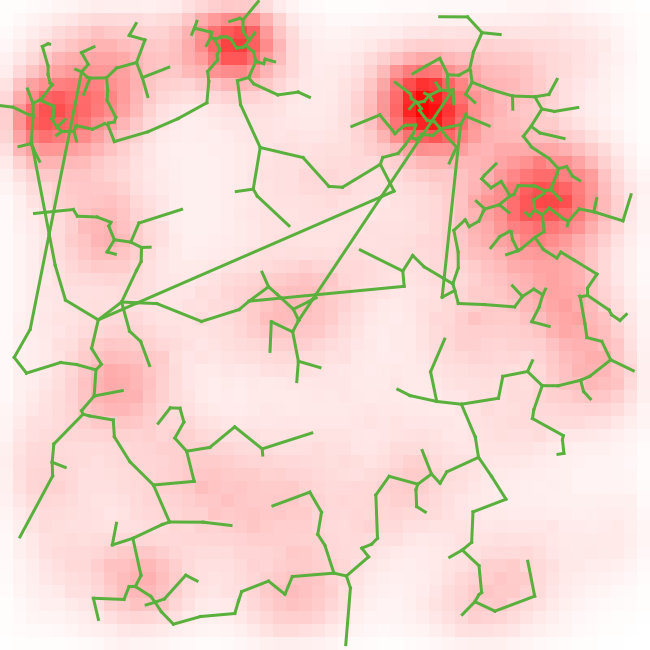
\includegraphics[width=\textwidth]{Figures/Cover/cover} \\ \vspace{3cm} % Picture

\mySubtitle \\ \medskip % Thesis subtitle
Under the supervision of \myProf and \myOtherProf \\ \medskip
%\myDegree \\
\myDepartment \\  \medskip
\myFaculty \\  \bigskip
%\myUni \\ \bigskip

\myTime\ -- \myVersion % Time and version

\vfill

\end{center}
\end{addmargin}

\end{titlepage} % Main title page

% Back of the title page

\thispagestyle{empty}

\hfill

\vfill

\noindent\myName: \textit{\myTitle,} \mySubtitle, %\myDegree, 
\textcopyright\ \myTime

% You may wish to do something with the back of the title page, such as including your supervisors, location or time frame of the work. Below is an example of doing so although you may want to tweak it to your liking.

%\bigskip

%\noindent\spacedlowsmallcaps{Supervisors}: \\
%\myProf \\
%\myOtherProf \\ 
%\mySupervisor

%\medskip \\

%\noindent\spacedlowsmallcaps{Location}: \\
%\myLocation

%\medskip \\

%\noindent\spacedlowsmallcaps{Time Frame}: \\
%\myTime
 % Back of the title page

%\cleardoublepage% Dedication

\thispagestyle{empty}
\refstepcounter{dummy}

\pdfbookmark[1]{Dedication}{Dedication} % Bookmark name visible in a PDF viewer

\vspace*{3cm}

\begin{center}
\emph{Ohana} means family. \\
Family means nobody gets left behind, or forgotten. \\ \medskip
--- Lilo \& Stitch    
\end{center}

\medskip

\begin{center}
Dedicated to the loving memory of Rudolf Miede. \\ \smallskip
1939\,--\,2005
\end{center} % Dedication page

%\cleardoublepage
% Abstract

%\renewcommand{\abstractname}{Abstract} % Uncomment to change the name of the abstract

\pdfbookmark[1]{Reading Notes}{Reading Notes} % Bookmark name visible in a PDF viewer

\begingroup
\let\clearpage\relax
\let\cleardoublepage\relax
\let\cleardoublepage\relax

\chapter*{Reading Notes}{Notes de Lecture}

\textit{This provisory Memoire must be read as a work in progress, as it details progresses after one year of Doctorate. Many parts are given at the state of project, and not omitted as playing a role in the current research questioning. Its purpose is to set up a plan and examine the achieved work and corresponding directions, but also to share research ideas at this important step of one year.}




\endgroup			

\vfill



 % Uncomment and create a Foreword.tex to include a foreword

\cleardoublepage% Abstract

%\renewcommand{\abstractname}{Abstract} % Uncomment to change the name of the abstract

\pdfbookmark[1]{Abstract}{Abstract} % Bookmark name visible in a PDF viewer

\begingroup
\let\clearpage\relax
\let\cleardoublepage\relax
\let\cleardoublepage\relax

\chapter*{Abstract}
%Short summary of the contents\dots a great guide by 
%Kent Beck how to write good abstracts can be found here:  
%\begin{center}
%\url{https://plg.uwaterloo.ca/~migod/research/beckOOPSLA.html}
%\end{center}









\endgroup			

\vfill % Abstract page

%\cleardoublepage% Publications - a page listing research articles written using content in the thesis

\pdfbookmark[1]{Publications}{Publications} % Bookmark name visible in a PDF viewer

\chapter*{Publications}{Publications} % Publications page text

%Some ideas and figures have appeared previously in the following publications:\\

%\noindent Put your publications from the thesis here. The packages \texttt{multibib} or \texttt{bibtopic} etc. can be used to handle multiple different bibliographies in your document.

%\begin{refsection}[ownpubs]
%    \small
%    \nocite{*} % is local to to the enclosing refsection
%    \printbibliography[heading=none]
%\end{refsection}

%\emph{Attention}: This requires a separate run of \texttt{bibtex} for your \texttt{refsection}, \eg, \texttt{ClassicThesis1-blx} for this file. You might also use \texttt{biber} as the backend for \texttt{biblatex}. See also \url{http://tex.stackexchange.com/questions/128196/problem-with-refsection}.

\bpar{
The following works have an highly overlapping content with this thesis:
}{
Les travaux suivants contiennent une grande partie du contenu de cette thèse:
}

% NOTE : on self-plagiarism, be careful to precise when extract from a published paper : 
%  - http://academia.stackexchange.com/questions/12342/self-plagiarism-in-phd-thesis
%  - http://academia.stackexchange.com/questions/2029/can-i-use-the-work-in-my-journal-conference-publications-as-chapters-in-my-disse
%  - http://academia.stackexchange.com/questions/149/what-is-a-sandwich-thesis


\section*{Publications}{Publications}


\noindent Antelope, C., Hubatsch, L., Raimbault, J., and Serna, J. M. (2016). An interdisciplinary approach to morphogenesis. Forthcoming in Proceedings of Santa Fe Institute CSSS 2016.


\bigskip

\noindent Raimbault, J. (2017). A Discrepancy-Based Framework to Compare Robustness Between Multi-attribute Evaluations. In Complex Systems Design \& Management (pp. 141-154). Springer International Publishing.

\bigskip

\noindent Raimbault, J. (2016). Investigating the Empirical Existence of Static User Equilibrium, \textit{forthcoming in EWGT 2016 proceedings, Transportation Research Procedia.} arxiv:1608.05266


\bigskip


\noindent Raimbault, J. (2016). Generation of Correlated Synthetic Data, forthcoming in \textit{Actes des Journ{\'e}es de Rochebrune 2016.}


\bigskip

\noindent Raimbault, J. (2015). Models Coupling Urban Growth and Transportation Network Growth: An Algorithmic Systematic Review Approach, forthcoming in \textit{ECTQG 2015 proceedings.} arxiv:1605.08888


\section*{Communications}{Communications}

\noindent Towards a Theory of Co-evolutive Networked Territorial Systems: Insights from Transportation Governance Modeling in Pearl River Delta, China, \textit{MEDIUM Seminar : Sustainable Development in Zhuhai, Guangzhou, Dec 2016.}


\bigskip


\noindent Models of growth for system of cities : Back to the simple, \textit{Conference on Complex Systems 2016, Amsterdam, Sep 2016.}



%Raimbault J., Bergeaud A. and Potiron Y. (2016). Investigating Patterns of Technological Innovation. \textit{Conference on Complex Systems 2016, Amsterdam, Sep 2016.}


\bigskip

\noindent For a Cautious Use of Big Data and Computation. \textit{Royal Geographical Society - Annual Conference 2016 - Session : Geocomputation, the Next 20 Years (1), London, Aug 2016.}


\bigskip

\noindent Indirect Bibliometrics by Complex Network Analysis. \textit{20e Anniversaire de Cybergeo, Paris, May 2016.}


\bigskip

\noindent Raimbault, J. \& Serra, H. (2016). Game-based Tools as Media to Transmit Freshwater Ecology Concepts, \textit{poster corner at SETAC 2016 (Nantes, May 2016).}


\bigskip

\noindent Le Néchet, F. \& Raimbault, J. (2015). Modeling the emergence of metropolitan transport authority in a polycentric urban region, \textit{ECTQG 2015, Bari, Sep 2015).}


\bigskip

\noindent Hybrid Modeling of a Bike-Sharing Transportation System, \textit{poster presented at ICCSS 2015, Helsinki, June 2015.}

\bigskip

\noindent Raimbault, J. \& Gonzales, J. (2015). Application de la Morphog{\'e}n{\`e}se de R{\'e}seaux Biologiques {\`a} la Conception Optimale d'Infrastructures de Transport, \textit{poster presented at Rencontres du Labex Dynamite, Paris, May 2015.}


 % Publications from the thesis page

%\cleardoublepage% Acknowledgements

\pdfbookmark[1]{Acknowledgements}{Acknowledgements} % Bookmark name visible in a PDF viewer

\begin{flushright}{\slshape    
We have seen that computer programming is an art, \\ 
because it applies accumulated knowledge to the world, \\ 
because it requires skill and ingenuity, and especially \\
because it produces objects of beauty.} \\ \medskip
--- \defcitealias{knuth:1974}{Donald E. Knuth}\citetalias{knuth:1974} \citep{knuth:1974}
\end{flushright}

\bigskip

%----------------------------------------------------------------------------------------

\begingroup

\let\clearpage\relax
\let\cleardoublepage\relax
\let\cleardoublepage\relax

\chapter*{Acknowledgements}

\noindent Put your acknowledgements here.\\

\noindent Many thanks to everybody who already sent me a postcard!\\

\noindent Regarding the typography and other help, many thanks go to Marco Kuhlmann, Philipp Lehman, Lothar Schlesier, Jim Young, Lorenzo Pantieri and Enrico Gregorio\footnote{Members of GuIT (Gruppo Italiano Utilizzatori di \TeX\ e \LaTeX )}, J\"org Sommer, Joachim K\"ostler, Daniel Gottschlag, Denis Aydin, Paride Legovini, Steffen Prochnow, Nicolas Repp, Hinrich Harms, Roland Winkler, and the whole \LaTeX-community for support, ideas and some great software.

\bigskip

\noindent\emph{Regarding \mLyX}: The \mLyX\ port was initially done by
\emph{Nicholas Mariette} in March 2009 and continued by
\emph{Ivo Pletikosi\'c} in 2011. Thank you very much for your work and the contributions to the original style.

\endgroup % Acknowledgements page

\pagestyle{scrheadings} % Show chapter titles as headings

\cleardoublepage% Table of Contents - List of Tables/Figures/Listings and Acronyms

\refstepcounter{dummy}

\pdfbookmark[1]{\contentsname}{tableofcontents} % Bookmark name visible in a PDF viewer

\setcounter{tocdepth}{1} % Depth of sections to include in the table of contents - currently up to subsections

\setcounter{secnumdepth}{2} % Depth of sections to number in the text itself - currently up to subsubsections

\manualmark
\markboth{\spacedlowsmallcaps{\contentsname}}{\spacedlowsmallcaps{\contentsname}}
\tableofcontents 
\automark[section]{chapter}
\renewcommand{\chaptermark}[1]{\markboth{\spacedlowsmallcaps{#1}}{\spacedlowsmallcaps{#1}}}
\renewcommand{\sectionmark}[1]{\markright{\thesection\enspace\spacedlowsmallcaps{#1}}}

\clearpage

\begingroup 
\let\clearpage\relax
\let\cleardoublepage\relax
\let\cleardoublepage\relax

%----------------------------------------------------------------------------------------
%	List of Figures
%----------------------------------------------------------------------------------------

\refstepcounter{dummy}
%\addcontentsline{toc}{chapter}{\listfigurename} % Uncomment if you would like the list of figures to appear in the table of contents
\pdfbookmark[1]{\listfigurename}{lof} % Bookmark name visible in a PDF viewer

\listoffigures

\vspace{8ex}
%\newpage

%----------------------------------------------------------------------------------------
%	List of Tables
%----------------------------------------------------------------------------------------

\refstepcounter{dummy}
%\addcontentsline{toc}{chapter}{\listtablename} % Uncomment if you would like the list of tables to appear in the table of contents
\pdfbookmark[1]{\listtablename}{lot} % Bookmark name visible in a PDF viewer

%\chapter*{List of Tables}

\phantomsection

\listoftables
        
\vspace{8ex}
\newpage
    
%----------------------------------------------------------------------------------------
%	List of Listings
%---------------------------------------------------------------------------------------- 

%\refstepcounter{dummy}
%\addcontentsline{toc}{chapter}{\lstlistlistingname} % Uncomment if you would like the list of listings to appear in the table of contents
%\pdfbookmark[1]{\lstlistlistingname}{lol} % Bookmark name visible in a PDF viewer

%\lstlistoflistings 

%\vspace{8ex}
%\newpage
       
%----------------------------------------------------------------------------------------
%	Acronyms
%----------------------------------------------------------------------------------------

%\refstepcounter{dummy}
%\addcontentsline{toc}{chapter}{Acronyms} % Uncomment if you would like the acronyms to appear in the table of contents
%\pdfbookmark[1]{Acronyms}{acronyms} % Bookmark name visible in a PDF viewer

%\markboth{\spacedlowsmallcaps{Acronyms}}{\spacedlowsmallcaps{Acronyms}}

%\chapter*{Acronyms}

%\begin{acronym}[ABM]
%\acro{ABM}{Agent-based Modeling}
%\acro{API}{Application Programming Interface}
%\acro{UML}{Unified Modeling Language}
%\end{acronym}  
             
             

%\begin{acronym}[SOC]
%\acro{ABM}{Self-organized Criticality}
%\end{acronym} 
             
             
             
                   
\endgroup % Contents, list of figures/tables/listings and acronyms

\cleardoublepage

\pagenumbering{arabic} % Arabic page numbering for thesis content (1, 2, 3, etc)
%\setcounter{page}{90} % Uncomment to manually start the page counter at an arbitrary value (for example if you wish to count the pre-content pages in the page count)

\cleardoublepage % Avoids problems with pdfbookmark

%----------------------------------------------------------------------------------------
%	THESIS CONTENT - CHAPTERS
%----------------------------------------------------------------------------------------


\part*{Introduction}





\ctparttext{} % Text on the Part 1 page describing  the content in Part 1

% Part I : methodology / theory / meta-theory
\part{} % First part of the thesis


%%%%%%%%%%%%%%%%%%%%%%%%%%%%%
% Chapter : Quantitative Epistemology


% Chapter 




\chapter{Quantitative Epistemology} % Chapter title

\label{ch:quantepistemo} % For referencing the chapter elsewhere, use \autoref{ch:name} 

%----------------------------------------------------------------------------------------


\headercit{something on knowledge}{}{}


A corollary of theoretical background proposed in chapter~\ref{ch:theory} is the need of an understanding of involved disciplines themselves to be able to build integrated heterogeneous models. The potentialities of couplings and integrations are greatly determined by existing approaches and corresponding gaps. This implies an advanced epistemological study in each field, that we propose to tackle in a systematic and quantitative way. This deliberate choice may shadow elaborated epistemological considerations but fits of purpose of preliminary investigations for the construction of models. 






%----------------------------------------------------------------------------------------


\newpage


\section{Algorithmic Systematic Review}


A broad bibliographical study suggests a scarcity of quantitative models of simulation integrating both network and urban growth. This absence may be due to diverging interests of concerned disciplines, resulting in a lack of communication.  We propose to proceed to an algorithmic systematic review to give quantitative elements of answer to this question. A formal iterative algorithm to retrieve corpuses of references from initial keywords, based on text-mining, is developed and implemented. We study its convergence properties and do a sensitivity analysis. We then apply it on queries representative of the specific question, for which results tend to confirm the assumption of disciplines compartmentalization.



\subsection{In search of models of co-evolution}


Transportation networks and urban land-use are known to be strongly coupled components of urban systems at different scales~\cite{bretagnolle2009organization}. One common approach is to consider them as co-evolving, avoiding misleading interpretations such as the myth of structural effect of transportation infrastructures~\cite{offner1993effets}. A question rapidly arising is the existence of models endogeneizing this co-evolution, i.e. taking into account simultaneous urban and network growth. We try to answer it using an algorithmic systematic review. We propose in this section, after a brief state of the art of existing literature, to present such an approach by formalizing the algorithm, which results are then presented and discussed. 

\subsection{Modeling Interactions between Urban Growth and Network Growth : An Overview}

\subsubsection{Land-Use Transportation Interaction Models.}

A wide class of models that have been developed essentially for planning purposes, which are the so-called Land-use Transportation Interaction Models, is a first type answering our research question. See recent reviews \cite{chang2006models}, \cite{iacono2008models} and \cite{wegener2004land} to get an idea of the heterogeneity of included approaches, that exist for more than 30 years. Recent models with diverse refinements are still developed today, such as \cite{delons:hal-00319087} which includes housing market for Paris area. Diverse aspects of the same system can be translated into many models (as \eg \cite{wegener1991one}), and traffic, residential and employment dynamics, resulting land-use evolution, influenced also by a static transportation network, are generally taken into account.

\subsubsection{Network Growth Approaches}

On the contrary, many economic literature has done the opposite of previous models, i.e. trying to reproduce network growth given assumptions on the urban landscape, as reviewed in \cite{zhang2007economics}. In~\cite{xie2009modeling}, economic empirical studies are positioned within other network growth approaches, such as work by physicists proposing model of geometrical network growth \cite{barthelemy2008modeling}. Analogy with biological networks was also done, reproducing typical robustness properties of transportation networks \cite{tero2010rules}.

\subsubsection{Hybrid Approaches}

Fewer approaches coupling urban growth and network growth can be found in the literature. \cite{barthelemy2009co} couples density evolution with network growth in a toy model. In~\cite{raimbault2014hybrid}, a simple Cellular Automaton coupled with an evolutive network reproduces stylized facts of human settlements described by Le Corbusier. At a smaller scale, \cite{achibet2014model} proposes a model of co-evolution between roads and buildings, following geometrical rules. These approaches stay however limited and rare.


\subsection{Bibliometric Analysis}

Literature review is a crucial preliminary step for any scientific work and its quality and extent may have a dramatic impact on research quality. Systematic review techniques have been developed, from qualitative review to quantitative meta-analyses allowing to produce new results by combining existing studies \cite{rucker2012network}. Ignoring some references can even be considered as a scientific mistake in the context of emerging information systems~\cite{lissacksubliminal}. We aim to take advantage of such techniques to tackle our issue.
Indeed, observing the form of the bibliography obtained in previous section raises some hypothesis. It is clear that all components are present for co-evolutive models to exist but different concerns and objectives seem to stop it. As it was shown by \cite{commenges:tel-00923682} for the concept of mobility, for which a ``small world of actors'' relatively closed invented a notion ad hoc, using models without accurate knowledge of a more general scientific context, we could be in an analog case for the type of models we are interested in. Restricted interactions between scientific fields working on the same objects but with different purposes, backgrounds and at different scales, could be at the origin of the relative absence of co-evolving models. 
While most of studies in bibliometrics rely on citation networks \cite{2013arXiv1310.8220N} or co-autorship networks \cite{2014arXiv1402.7268S}, we propose to use a less explored paradigm based on text-mining introduced in~\cite{chavalarias2013phylomemetic}, that obtain a dynamic mapping of scientific disciplines based on their semantic content. For our question, it has a particular interest, as we want to understand content structure of researches on the subject. We propose to apply an algorithmic method described in the following. The algorithm proceeds by iterations to obtain a stabilized corpus from initial keywords, reconstructing scientific semantic landscape around a particular subject.

\subsubsection{Description of the Algorithm}

Let $A$ be an alphabet, $A^{\ast}$ corresponding words and $T = \cup_{k\in \mathbb{N}} {A^{\ast}}^k$ texts of finite length on it. A reference is for the algorithm a record with text fields representing title, abstract and keywords. Set of references at iteration $n$ will be denoted $\mathcal{C} \subset T^3$. We assume the existence of a set of keywords $\mathcal{K}_n$, initial keywords being $\mathcal{K}_0$. An iteration goes as follows :

\begin{enumerate}
\item A raw intermediate corpus $\mathcal{R}_n$ is obtained through a catalog request providing previous keywords $\mathcal{K}_{n-1}$.
\item Overall corpus is actualized by $\mathcal{C}_n = \mathcal{C}_{n-1} \cup \mathcal{R}_n$.
\item New keywords $\mathcal{K}_n$ are extracted from corpus through Natural Language Processing treatment, given a parameter $N_k$ fixing the number of keywords.
\end{enumerate}

The algorithm stops when corpus size becomes stable or a user-defined maximal number of iterations has been reached. Fig. 1 shows the global workflow.



%%%%%%%%%%%%%%%%%%%%%%%%%%%%
\begin{figure}
\centering
\includegraphics[width=\textwidth]{Figures/PartI/QuantitativeEpistemo/schema_algo}
\caption[Systematic review algorithm workflow]{Global workflow of the algorithm, including implementation details : catalog request is done through Mendeley API ; final state of corpuses are RIS files.}
\label{fig:quantepistemo:algo}
\end{figure}
%%%%%%%%%%%%%%%%%%%%%%%%%%%%



%%%%%%%%%%%%%%%%%%%%%%%%%%%%
\subsubsection{Results}

\paragraph{Implementation}

Because of the heterogeneity of operations required by the algorithm (references organisation, catalog requests, text processing), it was found a reasonable choice to implement it in Java. Source code is available on the Github repository of the project1. Catalog request, consisting in retrieving a set of references from a set of keywords, is done using the Mendeley software API \cite{mendeley} as it allows an open access to a large database. Keyword extraction is done by Natural Language Processing (NLP) techniques, following the workflow given in \cite{chavalarias2013phylomemetic}, calling a Python script that uses \cite{bird2006nltk}.


\paragraph{Convergence and Sensitivity Analysis}

A formal proof of algorithm convergence is not possible as it will depend on the empirical unknown structure of request results and keywords extraction. We need thus to study empirically its behavior. Good convergence properties but various sensitivities to Nk were found as presented in Fig. 2. We also studied the internal lexical consistence of final corpuses as a function of keywords number. As expected, small number yields more consistent corpuses, but the variability when increasing stays reasonable.


%%%%%%%%%%%%%%%%%%%%%%%%%%%%
\begin{figure}
\centering
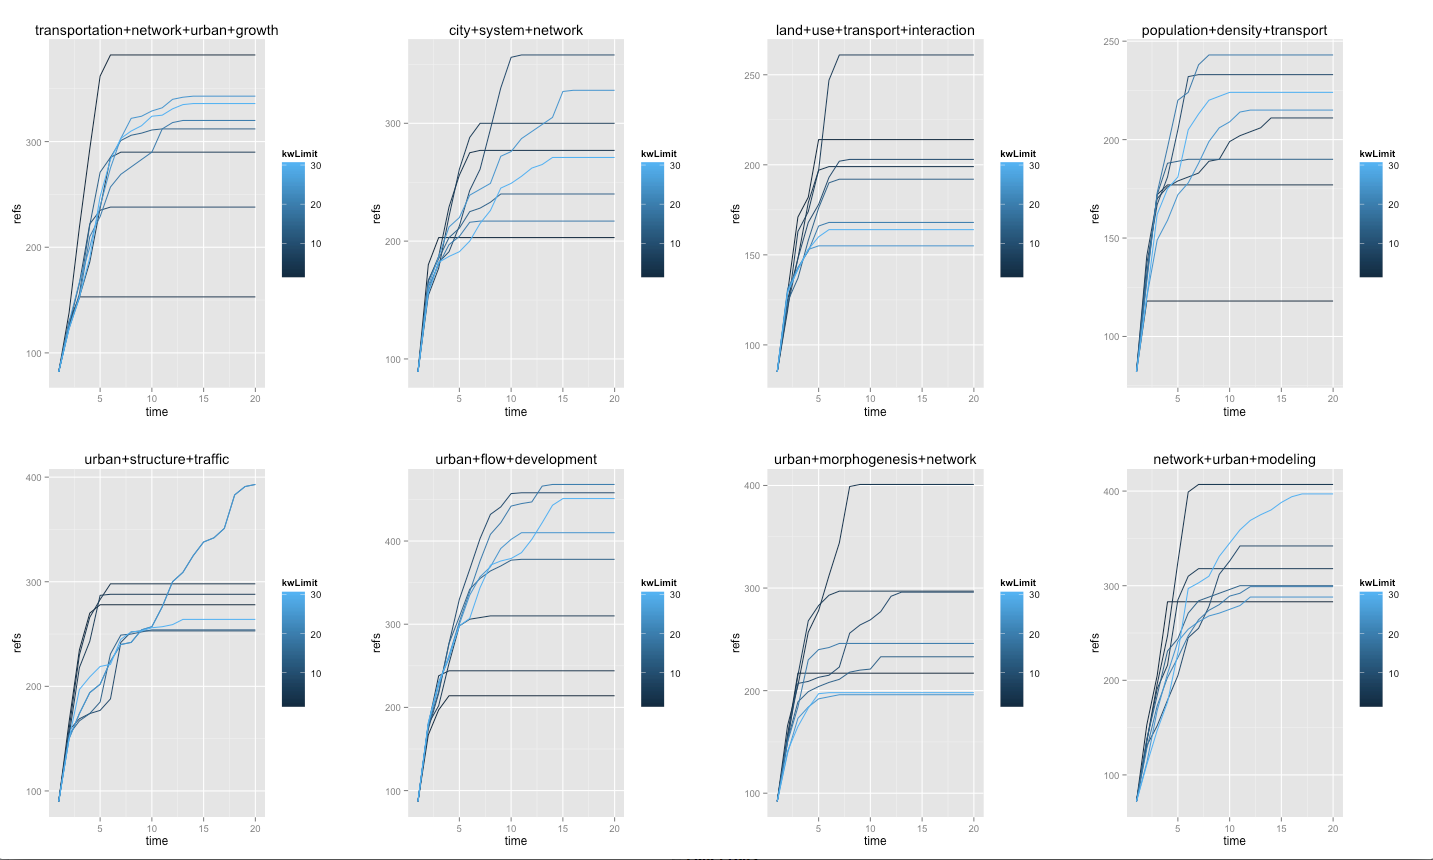
\includegraphics[width=\textwidth]{Figures/PartI/QuantitativeEpistemo/explo}
\medskip
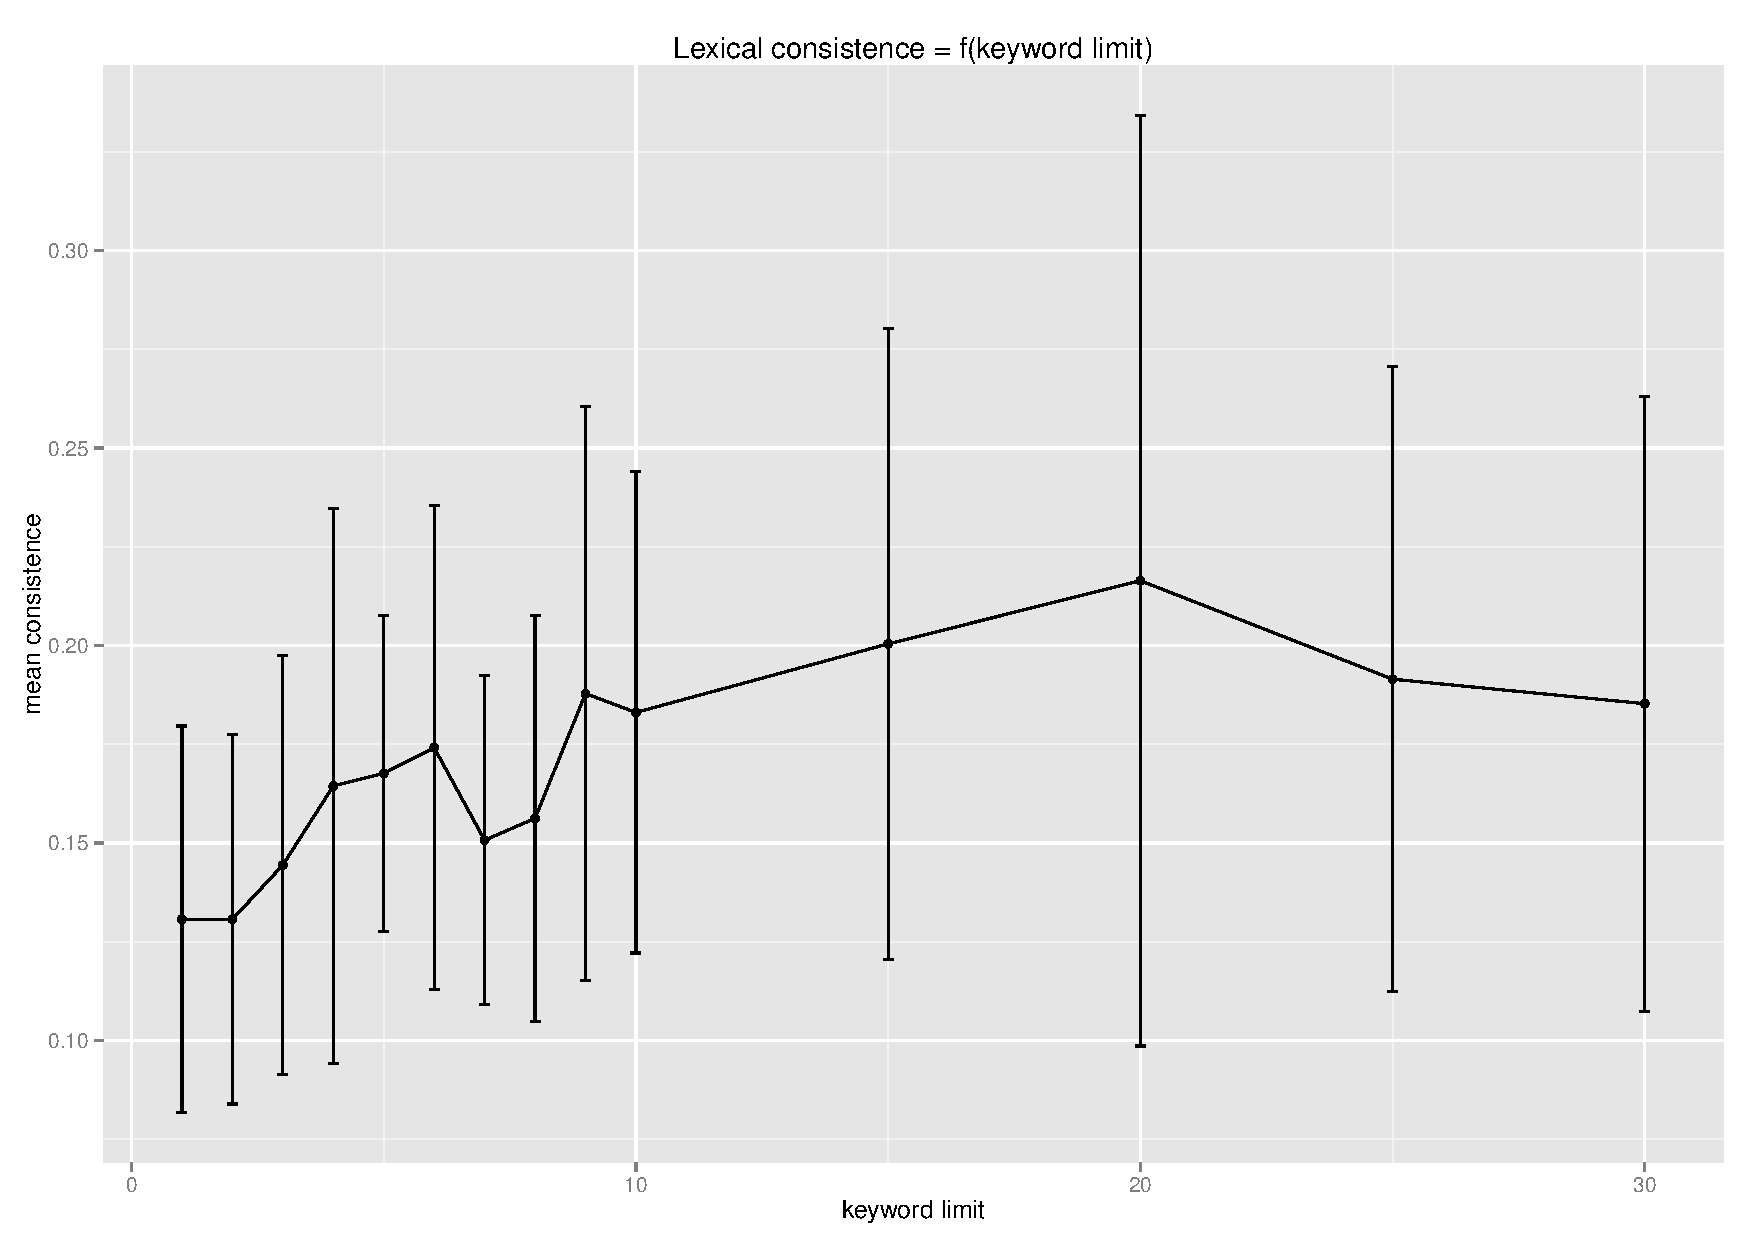
\includegraphics[width=0.8\textwidth]{Figures/PartI/QuantitativeEpistemo/lexicalConsistence_MeanSd}
\caption[Convergence and sensitivity analysis of systematic review algorithm]{Convergence and sensitivity analysis. Left : Plots of number of references as a function of iteration, for various queries linked to our theme (see further), for various values of $N_k$ (from 2 to 30). We obtain a rapid convergence for most cases, around 10 iterations needed. Final number of references appears to be very sensitive to keyword number depending on queries, what seems logical since encountered landscape should strongly vary depending on terms. Right : Mean lexical consistence and standard error bars for various queries, as a function of keyword number. Lexical consistence is defined though co-occurrences of keywords by, with $N$ final number of keywords, $f$ final step, and $c(i)$ co-occurrences in references, $k = \frac{2}{N(N-1)}\cdot \sum_{i,j \in \mathcal{K}_f}{\left| c(i) - c(j) \right|}$. The stability confirms the consistence of final corpuses.}
\label{fig:quantepistemo:sensitivity}
\end{figure}
%%%%%%%%%%%%%%%%%%%%%%%%%%%%




Once the algorithm is partially validated, we apply it to our question. We start from five different initial requests that were manually extracted from the various domains identified in the manual bibliography (that are ``city system network'', ``land use transport interaction'', ``network urban modeling'', ``population density transport'', ``transportation network urban growth''). We take the weakest assumption on parameter $N_k=100$, as it should less  constrain reached domains. After having constructed corpuses, we study their lexical distances as an indicator to answer our initial question. Large distances would go in the direction of the assumption made in section 2, i.e. that discipline self-centering may be at the origin of the lack of interest for co-evolutive models. We show in Table 1 values of relative lexical proximity, that appear to be significantly low, confirming this assumption.


\begin{table}
\centering
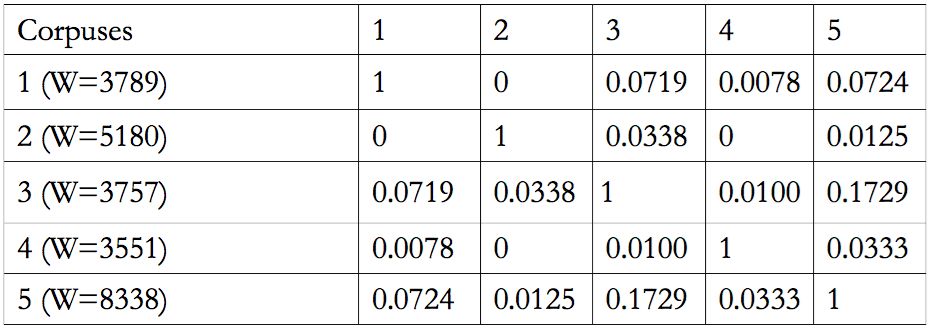
\includegraphics[width=\textwidth]{Figures/PartI/QuantitativeEpistemo/corpusesDistances}
\caption[Stationary lexical proximities]{Symmetric matrix of lexical proximities between final corpuses, defined as the sum of overall final keywords co-occurrences between corpuses, normalized by number of final keywords (100). We obtain very low values, confirming that corpuses are significantly far. Size of final corpuses is given as $W$.}
\end{table}



Further work is planned towards the construction of citation networks through an automatic access to Google Scholar that provides backward citations. The confrontation of inter-cluster coefficients on the citation network for the different corpuses with our lexical consistence results are an essential aspect of a further validation of our results.


The disturbing absence of models simulating the co-evolution of transportation networks and urban land-use, confirmed through a state-of-the-art covering many domain, may be due to the absence of communication between scientific disciplines studying different aspects of that problems. We have proposed an algorithmic method to give elements of answers through text-mining-based corpus extraction. First numerical results seem to confirm the assumption. However, such a quantitative analysis  should not be considered alone, but rather come as a back-up for qualitative studies that will be the object of further work, such as the one lead in~\cite{commenges:tel-00923682}, in which questionnaires with historical actors of modeling provide highly relevant information.





%--------------------------------------------------------------

\newpage

% Section describing cybergeo method.

\section{Refining bibliometrics through Hyper-network analysis}

%%%%%%%%%%%%%%
\subsection{Context}

As described before, semantic analysis does not contain all the information on disciplinary compartmentation nor on patterns of propagation of scientific knowledge as the ones contained in citation networks for example. Furthermore, data collection in the previous algorithm is subject to convergence towards self-consistent themes because of the proper structure of the method. It may give more insight about scientific social patterns of ontological choices in modeling to study communities in broader networks, that would more correspond to disciplines (or sub-disciplines depending on granularity level).

Previous works in quantitative epistemology using various types of networks have shown interesting potentialities. For the citation network, a good predicting power for citation patterns is for example obtained in~\cite{2013arXiv1310.8220N}. Co-authorship networks can also be used for predictive models~\cite{2014arXiv1402.7268S}. A multilayer network approach was recently proposed in~\cite{2016arXiv160106075O}, using bipartites networks of papers and scholars, in order to produce measures of interdisciplinarity. Disciplines can be stratified into layers to reveal communities between them and therein collaboration patterns~\cite{2015arXiv150601280B}.

\cite{10.1371/journal.pone.0147913}







%%%%%%%%%%%%%
\subsection{Application to a scientific journal}

\subsubsection{Presentation}

We briefly describe here an ongoing study that implemented the ideas given above for the particular case of a scientific journal for which bibliographical data is difficult to obtain, that is \texttt{cybergeo}, an electronic journal in theoretical and quantitative geography.


\cite{2015arXiv151003797G}
\cite{2016arXiv160208451P}
\cite{choi2014patent}
\cite{shibata2008detecting}


\subsubsection{Implementation}

The general architecture for data collection is presented in Fig.~\ref{fig:quantepistemo:data}. Citation data is collected from \texttt{Google Scholar}, that is the only source for incoming citations~\cite{noruzi2005google} in our case as the journal is not referenced in other databases. We are aware of the possible biaises using this single source~\cite{bohannon2014scientific}\footnote{or see \url{http://iscpif.fr/blog/2016/02/the-strange-arithmetic-of-google-scholars/}}, but these critics are more directed towards search results than citation counts. 



Text processing is done the same way as in previous section, expect that a particular treatment is done to language detection using \emph{stop-words} and a specific tagger \texttt{TreeTagger} is used for other languages than english~\cite{schmid1994probabilistic}.





%%%%%%%%%%%%%%%%%%
\begin{figure}
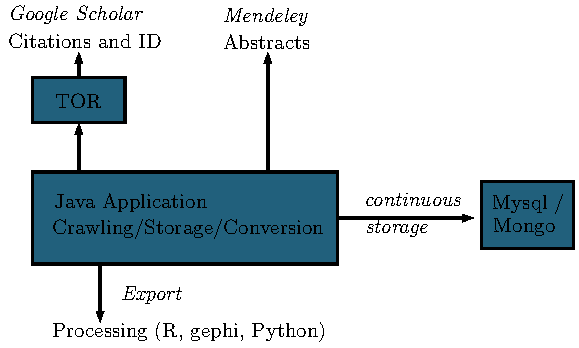
\includegraphics[width=\textwidth]{Figures/PartI/QuantitativeEpistemo/HyperNetwork/archi}
\caption[Heterogeneous Bibliographical Data Collection]{Heterogeneous Bibliographical Data Collection. Architecture of the application for content (semantic data), metadata and citation data collection.}
\label{fig:quantepistemo:data}
\end{figure}
%%%%%%%%%%%%%%%%%%


\subsubsection{Results}


We show in figures~\ref{fig:quantepistemo:citnw} and~\ref{fig:quantepistemo:semanticnw} preliminary results on citation and semantic network.

%%%%%%%%%%%%%%%%%
\begin{figure}
%\hspace{-3cm}
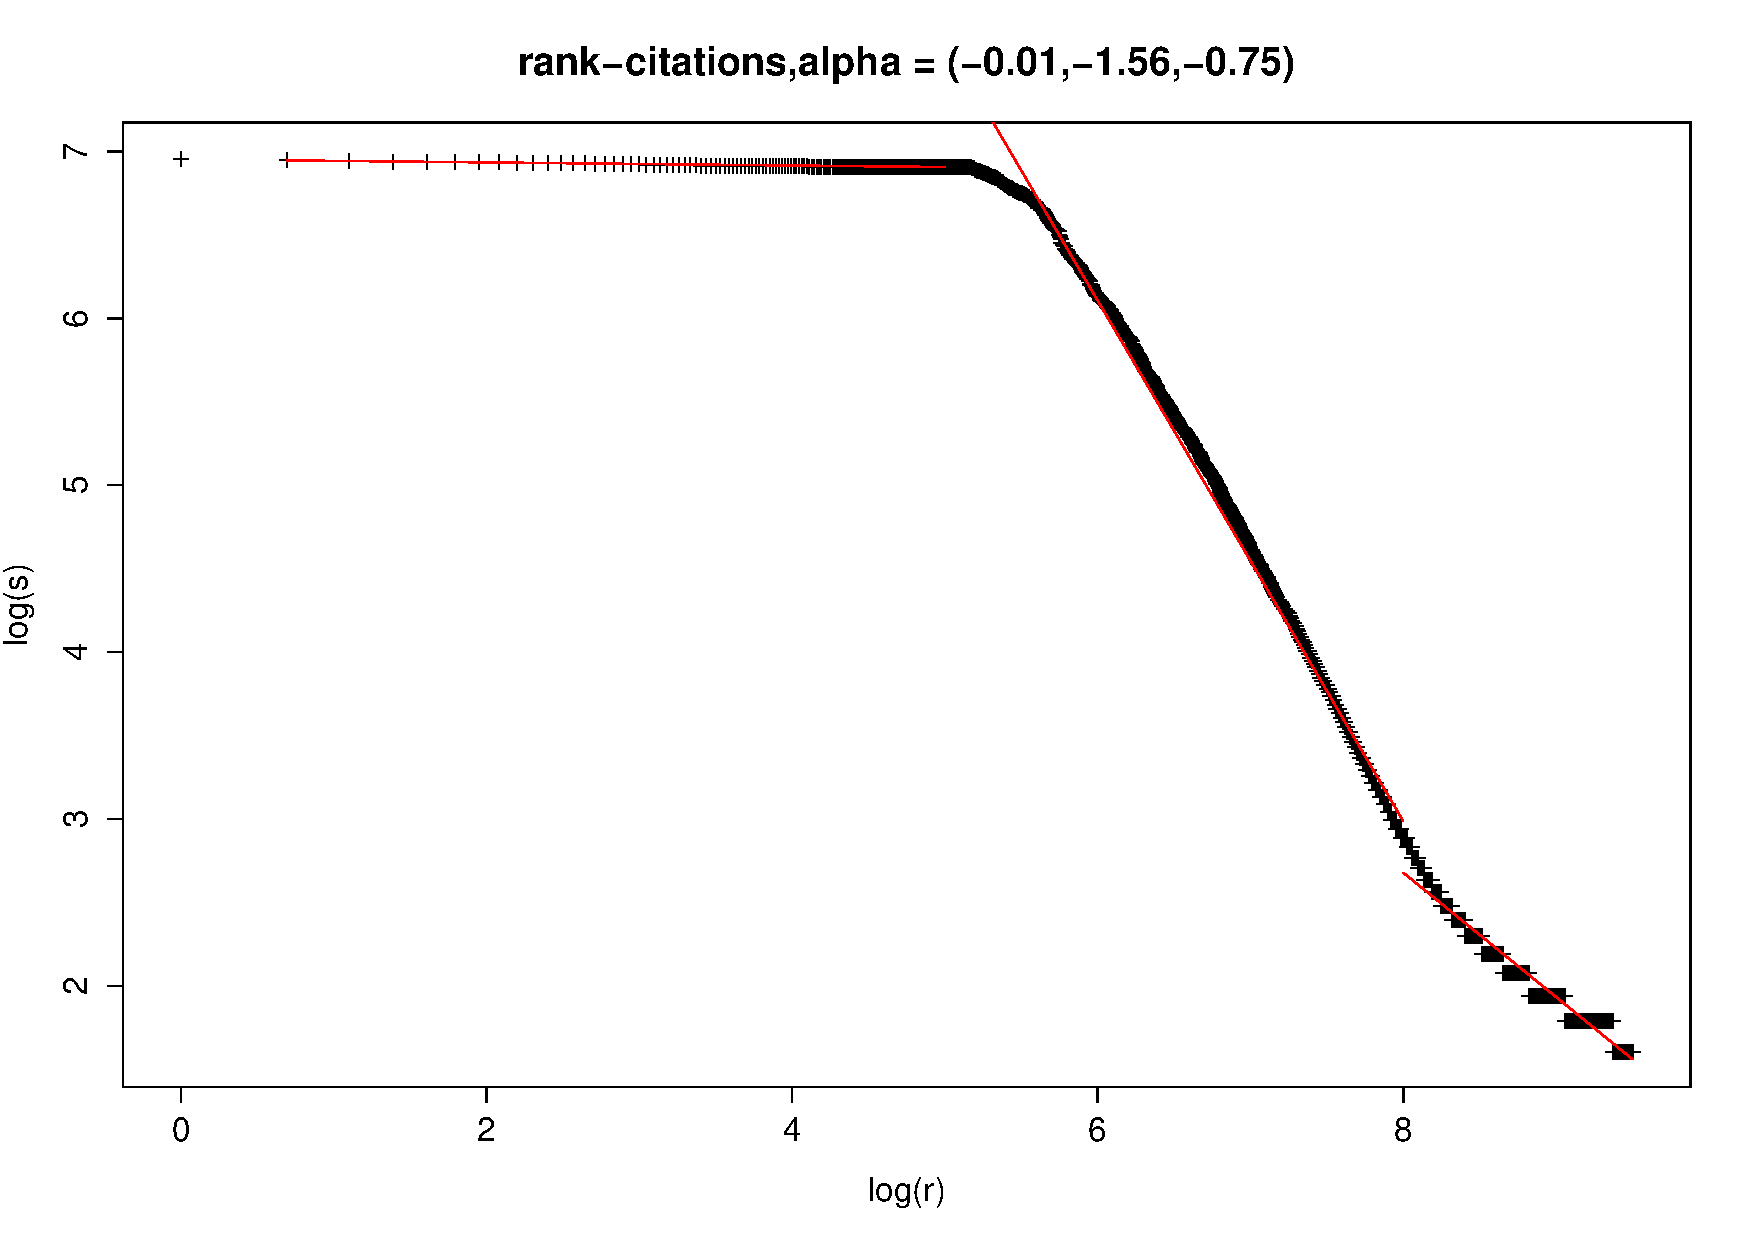
\includegraphics[width=\textwidth]{Figures/PartI/QuantitativeEpistemo/HyperNetwork/rank-size-all}
%\hspace{-3cm}
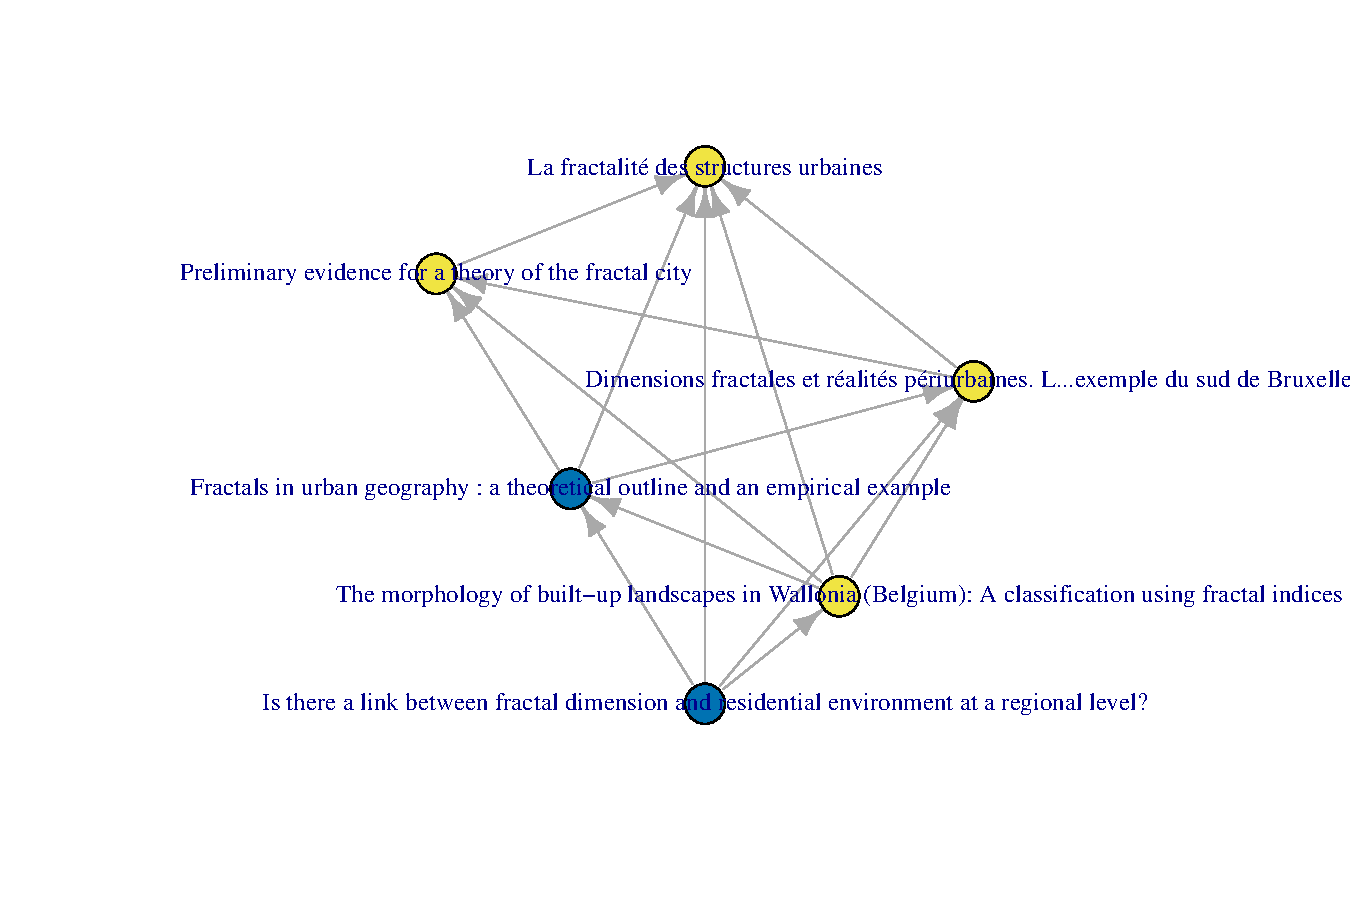
\includegraphics[width=\textwidth]{Figures/PartI/QuantitativeEpistemo/HyperNetwork/cybclic_2cyb_13761}
\caption[Properties of the citation network]{Properties of the citation network}
\label{fig:quantepistemo:citnw}
\end{figure}
%%%%%%%%%%%%%%%%%


%%%%%%%%%%%%%%%%%%
\begin{figure}
\hspace{-4cm}
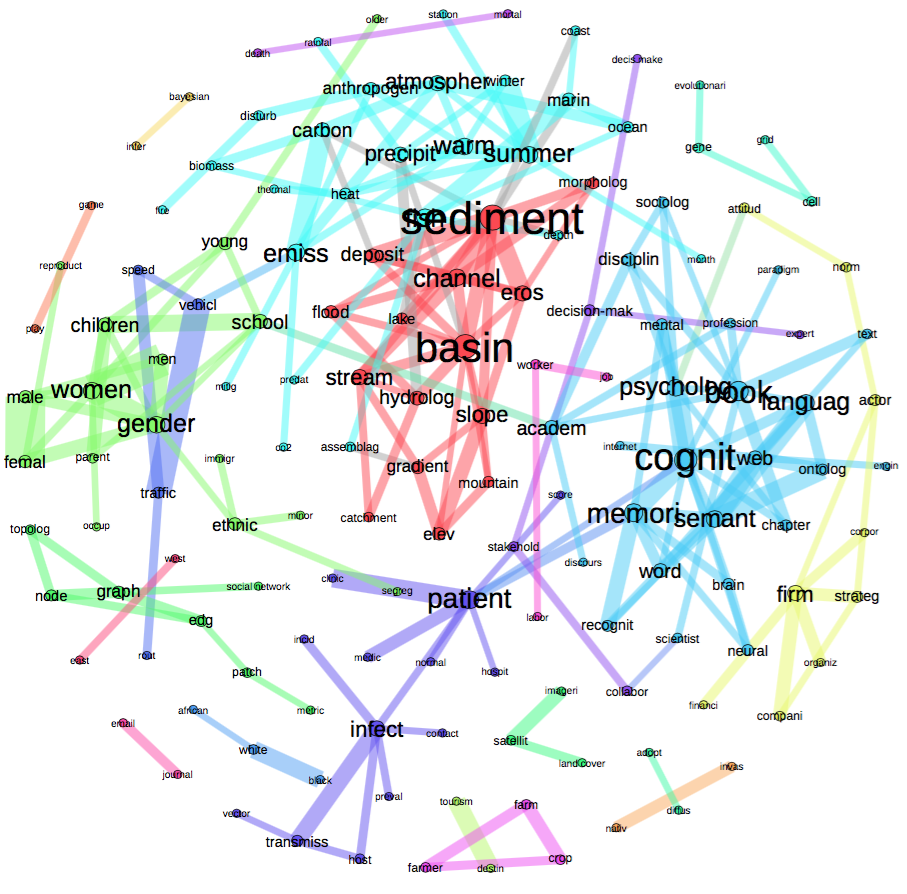
\includegraphics[width=1.4\textwidth]{Figures/PartI/QuantitativeEpistemo/HyperNetwork/all_lesslinks}
\caption[Semantic network of concepts in quantitative geography]{Semantic network of concepts in quantitative geography. Corpus consists of around $2\cdot 10^5$ abstracts of publications at a topological distance shorter than 2 from the journal \texttt{cybergeo} in the citation network. Relevance of keywords were estimated with the bootstrap method, }
\label{fig:quantepistemo:semanticnw}
\end{figure}
%%%%%%%%%%%%%%%%%%







%--------------------------------------------------------------

\newpage

%  Project section : describing ideas for more advanced text mining


\section{Towards modeling purpose and context automatic extraction}


A possible direction to strengthen our quantitative epistemological analysis would be to work on full textes related to the modeling of interaction between networks and territories, with the aim to automatically extract thematics within articles. The idea would be to perform some kind of automatized modelography, with possible features to be extracted that would be ontologies, model architecture or structures, scales, or even typical parameter values. It is not clear to what degree structure of models can be extracted from their description in papers and it surely depends on the discipline considered. For example in a framed field such as transportation planning, using a pre-defined ontology (in the sense of dictionary) and a fuzzy grammar could be efficient to extract information as the discipline is relatively formatted. In theoretical and quantitative geography, beyond the barrier of language, information organisation is surely less subject to unsupervised data-mining because of the more literary nature of the discipline : synonyms and style figures are generally the norm in good level human sciences writing, fuzzing a possible generic structure of knowledge description.

% cit LDA for thematic extraction ?









%%%%%%%%%%%%%%%%%%%%%%%%%%%%%




%%%%%%%%%%%%%%%%%%%%%%%%%%%%%
% Chapter : Quantitative Epistemology



% Chapter 

\chapter{Methodological Developments} % Chapter title

\label{ch:methodology} % For referencing the chapter elsewhere, use \autoref{ch:name} 

%----------------------------------------------------------------------------------------

\headercit{We are now building a rigorous Science of Cities, contrarily to what was done before.}{Marc Barth{\'e}l{\'e}my}{}

\bigskip

Such a shocking phrase was pronounced during the introduction of a \emph{Network} course for students of Complex System Science. Besides the fact that the spirit of CSS is precisely the opposite, {\ie} the construction of integrative disciplines (vertical integration that is necessarily founded on the existing body of knowledge of concerned fields) that answer transversal questions (horizontal integration that imply interdisciplinarity) - see {\eg} the roadmap for CS~\cite{2009arXiv0907.2221B}, it reveals how methodological considerations shape the perceptions of disciplines. From a background in Physics, ``rigorous'' implies the use of tools and methods judged more rigorous (analytical derivations, large datasets statistics, etc.). But what is rigorous for someone will not be for an other discipline\footnote{a funny but sad anecdote told by a friend comes to mind : defending his PhD in statistics, he was told at the end by economists how they were impressed by the mathematical rigor of his work, whereas a mathematician judged that ``he could have done everything on the back of an enveloppe''.}, depending on the purpose of each piece of research (perspectivism~\cite{giere2010scientific} poses the \emph{model}, that includes methods, as the articulating core of research entreprises). Thus the full role of methodology aside and not beside theory and experiments. We go in this chapter into various methodological developments which may be precisely used later or contribute to the global background.

We first propose a kind of essay insisting on the importance of reproducibility in science. More than a guideline, it is a way to practice science that a necessary condition for its rigor. Any non-reproducible work is not scientific. We then derive technical results on models of urban growth and on the sensitivity of scaling laws, that are both recurrent themes in the modeling of complex urban systems. We then introduce a method in the context of systematic model exploration and model behavior. We finally work on a link between static and dynamic correlations in a geographical system. This chapter is rather heteroclite as sections may correspond to a particular technical need at a point in the thesis, to global methodological directions, or global research directions.



%----------------------------------------------------------------------------------------

\newpage

% Section : Reproducibility


\section{Reproducibility}{Reproducibilité}




The strength of science comes from the cumulative and collective nature of research, as progresses are made as Newton said ``standing on the shoulder of giants'', meaning that the scientific enterprise at a given time relies on all the work done before and that advances would not be possible without constructing on it. It includes development of new theories, but also extension, testing or falsifiability of previous ones. In that context 





As scientific reproducibility is an essential requirement for any study, its practice seems to be increasing~\cite{stodden2010scientific} and technical means to achieve it are always more developed (as e.g. ways to make data openly available, or to be transparent on the research process such as \texttt{git}~\cite{ram2013git}, or to integrate document creation and data analysis such as \texttt{knitr}~\cite{xie2013knitr}), at least in the field of numerical modeling and simulation. However, the devil is indeed in the details and obstacles judged at first sight as minor become rapidly a burden for reproducing and using results obtained in some previous researches. We describe two cases studies where models of simulation are apparently highly reproducible but unveil as puzzles on which research-time balance is significantly under zero, in the sense that trying to exploit their results may cost more time than developing from scratch similar models.






%%%%%%%%%%%%%%%%%%%%%%%%%%%%%%%%%%
\subsection{On the Need to Explicit the Model}{Sur la Besoin d'expliciter le modèle}

A current myth is that providing entire source code and data will be a sufficient condition for reproducibility. It will work if the objective is to produce exactly same plots or statistical analysis, assuming that code provided is the one which was indeed used to produce the given results. It is however not the nature of reproducibility. First, results must be as much implementation-independent as possible for clear robustness purposes. Then, in relation with the precedent point, one of the purposes of reproducibility is the reuse of methods or results as basis or modules for further research (what includes implementation in another language or adaptation of the method), in the sense that reproducibility is not replicability as it must be adaptable~\cite{drummond2009replicability}.

Our first case study fits exactly that scheme, as it was undoubtedly aimed to be shared with and used by the community since it is a model of simulation provided with the Agent-Based simulation platform NetLogo~\cite{wilensky1999netlogo}. The model is also available online~\cite{de2007netlogo} and is presented as a tool to simulate socio-economic dynamics of low-income residents in a city based on a synthetic urban environment, generated to be close in stylized facts from the real town of Tijuana, Mexico. Beside providing the source code, the model appears to be poorly documented in the literature or in comments and description of the implementation. Comments made thereafter are based on the study of the urban morphogenesis part of the model (setup for the ``residential dynamics'' component) as it is our global context of study~\cite{raimbault2014vers}. In the frame of that study, source code was modified and commented, which last version is available on the repository of the project\footnote{at \texttt{https://github.com/JusteRaimbault/CityNetwork/tree/master/Models/Reproduction/UrbanSuite}}.




\paragraph{Rigorous Formalization}{Formalisation Rigoureuse}

An obvious part of model construction is its rigorous formalization in a formal framework distinct from source code. There is of course no universal language to formulate it~\cite{banos2013pour}, and many possibilities are offered by various fields (e.g. UML, DEVS, pure mathematical formulation). No paper nor documentation is provided with the model, apart from the embedded NetLogo documentation since it only thematically describes in natural language the ideas behind each step without developing more and provides information about role of different elements of the interface.

This formulation is a key for it to be understood, reproduced and adapted ; but it also avoids implementation biases such as
\begin{itemize}
\item Architecturally dangerous elements : in the model, world context is a torus and agents may ``jump'' in the euclidian representation, what is not acceptable for a 2D projection of real world. To avoid that, many tricky tests and functions were used, including unadvised practices (e.g. dead of agents based on position to avoid them jumping).
\item Lack of internal consistence : the example of the patch variable \texttt{land-value} used to represent different geographical quantities at different steps of the model (morphogenesis and residential dynamics), what becomes an internal inconsistence when both steps are coupled when option \texttt{city-growth?} is activated.
\item Coding errors : in an untyped language such as NetLogo, mixing types may conduct to unexpected runtime errors, what is the case of the patch variable \texttt{transport} in the model (although no error occurs in most of run configurations from the interface, what is more dangerous as the developer thinks implementation is secure). Such problems should be avoided if implementation is done from an exact formal description of the model.
\end{itemize}


\paragraph{Transparent Implementation}{Implémentation Transparente}

A totally transparent implementation is expected, including ergonomics in architecture and coding, but 

% TODO incomplete ?

\paragraph{Expected Model Behavior}{Comportement attendu du modèle}

Whatever the definition, a model can not be reduced to its formulation and/or implementation, as expected model behavior or model usage can be viewed as being part of the model itself. In the frame of \noun{Giere}'s perspectivism~\cite{giere2010scientific}, the definition of model includes the purpose of use but also the agent who aims to use it. Therefore a minimal explication of model behavior and exploration of parameter roles is highly advised to decrease chances of misuses or misinterpretations of it. It includes simple runtime charts that are immediate on the NetLogo platform, but also indicators computations to evaluate outputs of the model. It can also be improved visualizations during runtime and model exploration, such as showed in Fig.~\ref{fig:example_tij_viz}.



%%%%%%%%%%%%%%%%%%%%%
\begin{figure}
\centering
\hspace{-2cm}
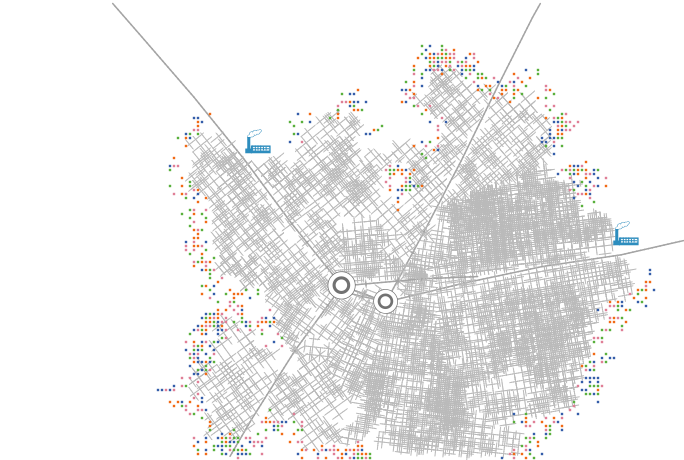
\includegraphics[width=0.33\textwidth]{Figures/PartI/Methodology/Reproducibility/stdView}
\hfill
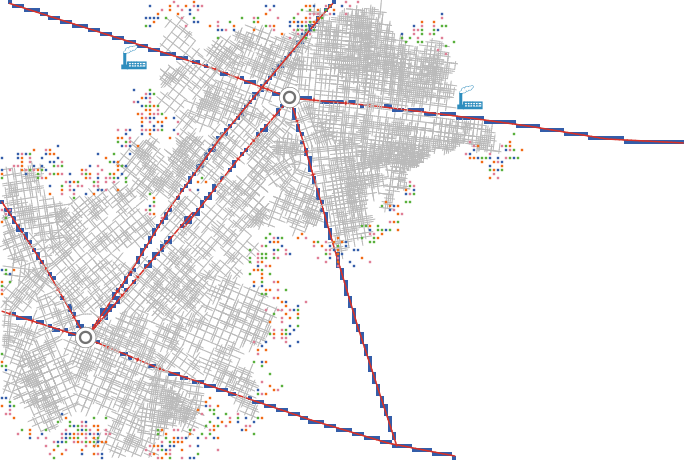
\includegraphics[width=0.33\textwidth]{Figures/PartI/Methodology/Reproducibility/ViewRoads}
\hfill
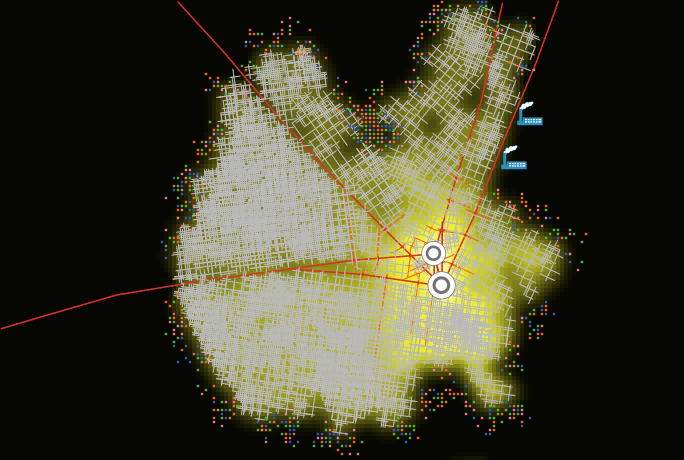
\includegraphics[width=0.33\textwidth]{Figures/PartI/Methodology/Reproducibility/landValues_cityFinished}
\caption[Reproducibility and visualization][Reproductibilité et visualisation]{Example of simple improvement in visualization that can help understanding mechanisms implied in the model. \textit{Left : } example of original output ; \textit{Middle : } visualization of main roads (in red) and underlying patches attribution, suggesting possible implementation bias in the use of discretized trace of roads to track their positions ; \textit{Right : }Visualization of land values using a more readable color gradient. This step confirms the hypothesis, through the form of value distribution, that the morphogenesis step is an unnecessary detour to generate a random field for which simple diffusion method should provide similar results, as detailed in the paragraph on implementation.}{}
\label{fig:example_tij_viz}
\end{figure}
%%%%%%%%%%%%%%%%%%%%%



\subsection{On the Need of Exactitude in Model Implementation}{Sue le besoin d'exactitude dans l'implémentation du modèle}

% Barthelemy paper, pb in model description/implementation
%  - test different analyses with possible biaises -

Possible divergences between model description in a paper and the effectively implemented processes may have grave consequences on the reproducibility of science. The road network growth model given in~\cite{barthelemy2008modeling} is one example that we are currently investigating. A strict implementation of model mechanisms provide slightly different results than the one presented in the paper, and as source code is not provided we need to test different hypotheses on possible mechanisms added by the programmer (that seems to be a connexion rule to intersections under a certain distance threshold). Lessons that could be possibly drawn from this examples are 
\begin{itemize}
\item the necessity of providing source code
\item the necessity of providing architecture description along with code (if model description is in a langage too far from architectural specifications) in order to identify possible implementation biaises
\item the necessity of performing and detailing explicitly model explorations, that would in that case have helped to identify the implementation bias.
\end{itemize}

The last point, if first not provided, may ensure a limited risk of scientific falsification as it may be more complicated to fake false exploration results than to effectively explore the model. A joint project currently done is the writing of a false modeling paper in the spirit of~\cite{zilsel2015canular}, in which opposite results to the effective results of a given model are provided, without providing model implementation. A first bunch of test is the acceptance of a clearly non-reproducible paper in diverse journals, possibly with a control on textual elements (using or not ``buzz-words'' associated to the journal, etc.). Depending on results, a second experiment may be tested with providing open source code for model implementation but still with false results, to verify if reviewers effectively try to reproduce results when they pretend to want the code (in reasonable computational power limits of course, HPC being not currently broadly available in Humanities).



\subsection{Perspectives}{Perspectives}


Again, reproducibility and transparency is a non-negotiable feature of contemporaneous science, along with Open practices and Open Access. Too much examples (see a very recent one in experimental economics~\cite{camerer2016evaluating}) show in various disciplines the lack of reproducibility of experiments, that is a falsification of previous results or a result in itself. Falsification is a costly practice, and even if necessary~\cite{chavalarias2005nobel}, could be made more efficient through more transparency and direct reproducibility, increase therein the global workflow of science. We develop in parallel of this thesis various tools aimed to ease reproducibility, for which an overview is given in appendix~\ref{app:workflow}.



%----------------------------------------------------------------------------------------

% Section : stochastic framework for urban growth


\newpage

\section{An unified framework for stochastic models of urban growth}{Un cadre unifié pour les modèles stichastiques de croissance urbaine}

Urban growth modeling fall in the case of tentatives to find self-consistent rules reproducing dynamics of an urban system, and thus in our logic of system morphogenesis. We examine here methodological issues linked to different frameworks of urban growth.

%%%%%%%%%%%%%%%%%%%%
\subsection{Introduction}{Introduction}
%%%%%%%%%%%%%%%%%%%%

Various stochastic models aiming to reproduce population patterns on large temporal and spatial scales (city systems) have been discussed across various fields of the literature, from economics to geography, including models proposed by physicists. We propose here a general framework that allows to include different famous models (in particular Gibrat, Simon and Preferential Attachment model) within an unified vision. It brings first an insight into epistemological debates on the relevance of models. Furthermore, bridges between models lead to the possible transfer of analytical results to some models that are not directly tractable.


Seminal models of urban growth are Simon~\cite{simon1955class} (later generalized as e.g. \cite{haran1973modified}) and Gibrat models. Many examples can be given across disciplines. \cite{benguigui2007dynamic} give an equation-based dynamical model, whereas \cite{gabaix1999zipf} solves a stationary model. \cite{Gabaix20042341} reviews urban growth approaches in economics. A model adapted from evolutive urban theory is solved in~\cite{favaro2011gibrat} and improves Gibrat models. The question of empirical scales at which it is consistent to study urban growth was also tackled in the particular case of France~\cite{bretagnolle2002time}. We stay to a certain level of tractability to include models as essence of our approach is links between models but do not make ontologic assumptions.




%%%%%%%%%%%%%%%%%%%%
\subsection{Framework}{Cadre de Travail}
%%%%%%%%%%%%%%%%%%%%


\paragraph{Presentation}
What we propose as a framework can be understood as a meta-model in the sense of~\cite{cottineau2015incremental}, i.e. an modular general modeling process within each model can be understood as a limit case or as a specific case of another model. More simply it should be a diagram of formal relations between models. The ontological aspect is also tackled by embedding the diagram into an ontological state space (which discretization corresponds to the ``bricks'' of the incremental construction of~\cite{cottineau2015incremental}). It constructs a sort of model classification or modelography.

We are still at the stage of different derivations of links between models that are presented hereafter.

%\subsubsection{Models Included}

%The following models are included in our framework. The list is arbitrary but aims to offer a broad view of disciplines concerned

%\subsubsection{Thematic Classification}


%\subsubsection{Framework Formulation}
%Diagram linking various models ; first embedded into time/population plane, cases Discrete/Continous. Other aspects more sparse (ex. spatialization) ; how represent it ?

%%%%%%%%%%%%%%%%%%%%
%\subsection{Models formulation}



%%%%%%%%%%%%%%%%%%%%
\subsection{Derivations}{Dérivations}

\subsubsection{Generalization of Preferential Attachment}{Généralisation de l'Attachement Préférentiel}

\cite{yamasaki2006preferential} give a generalization of the classical Preferential Attachment Network Growth model, as a birth and death model with evolving entities. More precisely, network units gain and lose population (equivalent to links connexions) at fixed probabilities, and new unit can be created at a fixed rate.

\subsubsection{Link between Gibrat and Preferential Attachment Models}{Lien entre Gibrat et Attachement Préférentiel}


\bpar{
Let consider a strictly positive growth Gibrat model given by $P_i(t)=R_i(t)\cdot P_{i}(t-1)$ with $R_i(t)>1$, $\mu_i(t)=\Eb{R_i(t)}$ and $\sigma_i(t)=\Eb{R_i(t)^2}$. On the other hand, we take a simple preferential attachment, with fixed attachment probability $\lambda \in [0,1]$ and new arrivants number $m>0$. We derive that Gibrat model can be statistically equivalent to a limit of the preferential attachment model, assuming that the moment-generating function of $R_i(t)$ exists. Classical distributions that could be used in that case, e.g. log-normal distribution, are entirely defined by two first moments, making this assumption reasonable.
}{
Considérons un modèle de croissance strictement positive de Gibrat donnée par $P_i(t)=R_i(t)\cdot P_{i}(t-1)$ avec $R_i(t)>1$, $\mu_i(t)=\Eb{R_i(t)}$ et $\sigma_i(t)=\Eb{R_i(t)^2}$. D'autre part, soit un modèle simple d'attachement préférentiel, avec une probabilité d'attachement $\lambda \in [0,1]$ et un nombre de nouveau arrivants $m>0$. Il est possible de dériver que le Gibrat est statistiquement équivalent à une limite de l'attachement préférentiel, sous l'hypothèse que toutes les fonctions génératrices des moments de $R_i(t)$ existent. Les distributions classiques qui peuvent être utilisées dans ce cas, e.g. une distribution normale ou log-normale, sont entièrement déterminées par leur deux premiers moments, ce qui rend cette hypothèse raisonnable.
}



\begin{lemma}
The limit of a Preferential Attachment model when $\lambda \ll 1$ is a linear-growth Gibrat model, with limit parameters $\mu_i(t)=1+\frac{\lambda}{m\cdot (t-1)}$.
\end{lemma}


\bpar{
The proof is given in Appendix~\ref{app:technical}.
}{
La preuve est donnée en Annexe~\ref{app:technical}.
}


\subsubsection{Link between Simon and Preferential Attachment}{Lien entre Simon et Attachement Préférentiel}
%\label{subsubsec:gibrat-simon}

A rewriting of Simon model yields a particular case of the generalized preferential attachment, in particular by vanishing death probability.

\subsubsection{Link between Favaro-Pumain and Gibrat}{Lien entre Favaro-Pumain et Gibrat}

\cite{favaro2011gibrat} generalizes Gibrat models with innovation propagation dynamics, being therefore a generalization of that model. Theoretically, a process-based model equivalent to the Favaro-pumain should then fill the missing case in model classification at the corresponding discretization. Simpop models do not fill that case as they stay at the scale of city systems, as for Marius models~\cite{cottineau2014evolution}. These must also have their counterparts in discrete microscopic formulation.

\subsubsection{Link between Bettencourt-West and Pumain}{Lien entre Bettencourt-West et Pumain}

We are considering to study Bettencourt-West model for urban scaling laws \cite{bettencourt2008large} as entering the stochastic urban growth framework as stationary component of a random growth model, but investigation are still ongoing.


\subsubsection{Other Models}{Autres modèles}

\cite{gabaix1999zipf} develops an economic model giving a Simon equivalent formulation. They in particular find out that in upper tail, proportional growth process occurs. We find the same result as a consequence of the derivation of the link between Gibrat and Preferential attachment models.




%%%%%%%%%%%%%%%%%%%%
%\subsection{Application and Perspectives}
%%%%%%%%%%%%%%%%%%%%







%%%%%%%%%%%%%%%%%%%%
%\subsection{Discussion}
%%%%%%%%%%%%%%%%%%%%

%%%%%%%%%%%%%%%%%%%%
%\subsection*{Conclusion}
%%%%%%%%%%%%%%%%%%%%





%----------------------------------------------------------------------------------------

\newpage


%  section : scaling sensitivity : useful ?


\section{Sensitivity of Urban Scaling Laws to Spatial Extent}{Sensibilité des Lois d'Echelle Urbaines à l'Etendue Spatiale}


\bpar{
At the center of evolutive urban theory are hierarchy and associated scaling laws. We develop here a brief methodological investigation on the sensitivity of scaling laws to city definition.
}{
Au centre de la théorie évolutive des villes se trouvent la hiérarchie et les lois d'échelle associées. Nous proposons ici un bref développement méthodologique sur la sensibilité des lois d'échelle à la définition de la ville.
}


%%%%%%%%%%%%%%%%%%%%
%\subsection{Introduction}



\bpar{
Scaling laws have been shown to be universal of urban systems at many scales and for many indicators. Recent studies question however the consistence of scaling exponents determination, as their value can vary significantly depending on thresholds used to define urban entities on which quantities are integrated, even crossing the qualitative border of linear scaling, from infra-linear to supra-linear scaling. We use a simple theoretical model of spatial distribution of densities and urban functions to show analytically that such behavior can be derived as a consequence of the type of spatial distribution and the method used. Numerical simulation confirm the theoretical results and reveals that results are reasonably independent of spatial kernel used to distribute density.
}{
Les lois d'échelle ont été montrées universelles des systèmes urbains à de nombreuses échelles et pour différents indicateurs. Des études récentes questionnent toutefois la cohérence de la détermination des exposants d'échelle, puisque leur valeur peut varier significativement selon les seuils utilisés pour définir les entités urbaines sur lesquelles les quantités urbaines sont intégrées, franchissant même dans certains cas la barrière qualitative de l'échelle linéaire, d'une loi infra-linéaire à une loi super-linéaire. Nous utilisons un modèle théorique simple de distribution spatiale des densités et des fonctions urbaines pour montrer analytiquement qu'un tel comportement peut être dérivé comme conséquence du type de distribution spatiale et de la méthode utilisée. Les simulations numériques confirment les résultats théoriques et révèle que les résultats sont raisonnablement indépendants du noyau spatial utilisé pour distribuer la densité.
}


\bpar{
Scaling laws for urban systems, starting from the well-known rank-size Zipf's law for city size distribution~\cite{gabaix1999zipf}, have been shown to be a recurrent feature of urban systems, at many scales and for many types of indicators. They reside in the empirical constatation that indicators computed on elements of an urban system, that can be cities for system of cities, but also smaller entities at a smaller scale, do fit relatively well a power-law distribution as a function of entity size, i.e. that for entity $i$ with population $P_i$, we have for an integrated quantity $A_i$, the relation $A_i \simeq A_0\cdot \left(\frac{P_i}{P_0}\right)^{\alpha}$. Scaling exponent $\alpha$ can be smaller or greater than 1, leading to infra or supralinear effects. Various thematic interpretation of this phenomena have been proposed, typically under the form of processes analysis. The economic literature has produced abundant work on the subject (see~\cite{Gabaix20042341} for a review), but that are generally weakly spatial, thus of poor interest to our approach that deals precisely with spatial organization. Simple economic rules such as energetic equilibria can lead to simple power-laws~\cite{bettencourt2008large} but are difficult to fit empirically. A interesting proposition by \noun{Pumain} is that they are intrinsically due to the evolutionary character of city systems, where complex emergent interaction between cities generate such global distributions~\cite{pumain2006evolutionary}. Although a tempting parallel can be done with self-organizing biological systems, \noun{Pumain} insists on the fact that the ergodicity assumption for such systems is not reasonable in the case of geographical systems and that the analogy can difficultly be exploited~\cite{pumain2012urban}. Other explanations have been proposed at other scales, such as the urban growth model at the mesoscopic scale (city scale) given in~\cite{2014arXiv1401.8200L} % TODO is this quote also relevant here ?
 that shows that the congestion within transportation networks may be one reason for city shapes and corresponding scaling laws. Note that ``classic'' urban growth models such as Gibrat's model do provide first order approximation of scaling systems, but that interactions between agents have to be incorporated into the model to obtain better fit on real data, such as the Favaro-Pumain model for innovation cycles propagation proposed in~\cite{favaro2011gibrat}, that generalize a Gibrat model for French cities with an ontology similar to Simpop models.
}{
Les lois d'échelle pour les systèmes urbains, en commençant par la bien connue loi rang-taille de Zipf pour la distribution des tailles des villes~\cite{gabaix1999zipf}, ont été montrées être une caractéristique récurrente des systèmes urbains, à différentes échelles et pour différents types d'indicateurs. Elles reposent sur la constatation empirique que des indicateurs calculés sur des éléments du système urbain, qui peuvent être les villes dans le cas d'un système de villes, mais aussi des entités plus petites à une plus petite échelle, suivent relativement bien une distribution en loi de puissance en fonction de la taille de l'entité, i.e. pour l'entité $i$ avec population $P_i$, on a pour une quantité intégrée $A_i$, la relation $A_i \simeq A_0\cdot \left(\frac{P_i}{P_0}\right)^{\alpha}$. Les exposants d'échelle $\alpha$ peuvent être plus petits ou plus grands que 1, menant à des effets infra ou supra-linéaires. Diverses interprétations thématiques de ce phénomène ont été proposées, typiquement sous la forme d'analyse des processus. La littérature économique contient une production abondante sur le sujet (voir~\cite{Gabaix20042341} pour une revue), mais est généralement faiblement spatiale, donc de faible intérêt pour notre approche qui s'intéresse particulièrement à l'organisation spatiale. Des règles économiques simples comme un équilibre énergétique peut conduire à de simples lois d'échelles~\cite{bettencourt2008large} mais sont difficiles à ajuster empiriquement. Une proposition intéressante par \noun{Pumain} est qu'elles sont intrinsèquement dues au caractère évolutionnaire des systèmes de villes, où l'émergence complexe par les interactions entre villes génère de telles distributions globales~\cite{pumain2006evolutionary}. Même si un parallèle tentant peut être fait avec les système biologiques auto-organisés % TODO here make a link with morphogenesis - depending if introduced before or not
 , \noun{Pumain} insiste sur le fait que l'hypothèse d'ergodicité pour de tels systèmes n'est pas raisonnable dans le cas de système géographiques et que l'analogie est difficilement exploitable~\cite{pumain2012urban}. D'autres explications ont été proposées à d'autres échelles, comme le modèle de croissance urbaine à échelle mesoscopique (échelle de la ville) donné dans~\cite{2014arXiv1401.8200L} qui montre que la congestion dans les réseaux de transport pourrait être une raison de la forme des villes et des lois d'échelle correspondantes. On peut noter que les modèles ``classiques'' de croissance urbaine comme le modèle de Gibrat~\cite{favaro2011gibrat} fournissent une approximation au premier ordre des systèmes % scaling systems = systèmes scalant ? ~ systèmes exhibant des lois d'échelle <- too long..
  exhibant des lois d'échelles, mais que les interactions entre agents doivent être incorporées dans le modèle pour obtenir un résultat plus fidèle aux données réelles, comme le modèle de Favaro-Pumain pour la propagation des cycles d'innovation proposé dans~\cite{favaro2011gibrat}, qui généralise un modèle de Gibrat pour la croissance des villes françaises avec une ontologie similaire à celle des modèles Simpop.
}


% TODO IDEE - take the FavaroPumain again, try to fit/compare with the IntGib-network model ? -- sort of benchmark, should be easy to implement


\bpar{
However, the blind application of scaling exponents computations was recently pointed as misleading in most cases~\cite{louf2014scaling} % TODO do not cite this empty "paper"
, confirmed by empirical works such as~\cite{2013arXiv1301.1674A} that showed the variability of computed exponents to the parameters defining urban areas, such as density thresholds. An ongoing work by Cottineau \& \textit{al.} presented at~\cite{cottineau2015scaling}, studies empirically for French Cities the influence of 3 parameters playing a role in city definition, that are a density threshold $\theta$ to delimitate boundaries of an urban area, a number of commuters threshold $\theta_c$ that is the proportion of commuters going to core area over which the unity is considered belonging to the area, and a cut-off parameter $P_c$ under which entities are not taken into account for the linear regression providing the scaling exponent. Remarquable results are that exponents can significantly vary and move from infra-linear to supra-linear when threshold varies. A systematic exploration of parameter space produces phase diagrams of exponents for various quantities. One question raising immediately is how these variation can be explained by the features of spatial distribution of variables. Do they result from intrinsic mechanisms present in the system or can they be explained more simply by the fact that the system is particularly spatialized ? We prove on a toy analytical model that even simple distributions can lead to such significant variations in the exponents, along one dimension of parameters (density threshold), directing the response towards the second explanation.
}{

}





%The rest of the section is organized as follows : we formalize the simple framework used and derive an analytical relation between estimated exponent and density threshold parameter. We then present a numerical implementation of the model that confirms numerically theoretical results, explore other form of kernels that would be less tractable, and study the sensitivity along two parameters. We finally discuss the implications of our results and further work needed.

The derivations in the simple case of exponential mixture density, are done in Appendix~\ref{app:technical}.

% TODO : mention way of fitting ; golden standard to fit power laws ? check thèse d'Olivier pour voir si le cutoff est appliqué ?







%----------------------------------------------------------------------------------------


\newpage


%  section : synthetic data control - introduces rochebrune paper, feasible correlation space etc, and forthcoming applications ?


\section{Statistical Control on Initial Conditions by Synthetic Data Generation}{Contrôle statistique pour les conditions initiales par génération de données synthétiques}

\subsection{Context}{Contexte}

When evaluating data-driven models, or even more simple partially data-driven models involving simplified parametrization, an unavoidable issue is the lack of control on ``underlying system parameters'' (what is a ill-defined notion but should be seen in our sense as parameters governing system dynamics). Indeed, a statistics extracted from running the model on enough different datasets can become strongly biased by the presence of confounding in the underlying real data, as it is impossible to know if result is due to processes the model tries to translate or to a hidden structure common to all data.

%Let illustrate the issue with a simple example.

We formalize briefly a proposition of method that would allow to add controls on meta-parameters, in the sense of parameters driving the represented system at a higher temporal and spatial scale, for a model of simulation. We make the hypothesis that such method is valid under constraints of disjonction for scales and/or ontologies between the model of simulation and the domain of meta-parameters.


\subsection{Description}{Description}

An advanced knowledge of the behavior of computational models on their parameter space is a necessary condition for deductions of thematic conclusions or their practical application~\cite{banos2013pour}. But the choice of varying parameters is always subjective, as some may be fixed by a real-world parametrization, or other may be interpreted as arbitrarily fixed initial conditions. It raises methodological and epistemological issues for the sensitivity analysis, as the scope of the model may become ill-defined.

Let consider the concrete example of the Schelling Segregation model~\cite{schelling1971dynamic}. One of its crucial features on which the literature has been rather controversial is the influence of the spatial structure of the container on which agents evolve.%~(\textit{Biblio Marion}). 
 The thematic aim of the project developed in~\cite{cottineau2015revisiting} is to clarify this point through a systematic model exploration. A methodological contribution is the construction of a framework allowing the analysis of the sensitivity of models to \emph{meta-parameters}, i.e. to parameters considered as fixed initial conditions (e.g. the spatial structure for the Schelling model), or to parameters of another model generating an initial configuration%, as detailed in Fig.~\ref{} \textit{[insert scheme describing the approach]}, 
 yielding thus a \emph{simple coupling} between models (serial coupling). The benefits of such an approach are various but include for example the knowledge of model behavior in an extended frame, the possibility of statistical control when regressing model outputs, a finer exploration of model derivatives than with a naive approach. Some remarks can be made on the approach :
\begin{itemize}
\item What knowledge are brought by adding the upstream model, rather than for example in the Schelling case exploring a large set of initial geometries ? 

$\rightarrow$ \textit{to obtain a sufficiently large set of initial configuration, one quickly needs a model to generate them ; in that case a quasi-random generation followed by a filtering on morphological constraint will be a morphogenesis model, which parameters are the ones of the generation and the filtering methods. Furthermore, as detailed further, the determination of the derivative of the downstream model is made possible by the coupling and knowledge of the upstream model.}
\item Statistical noise is added by coupling models

$\rightarrow$ \textit{Repetitions needed for convergence are indeed larger as the final expectance has to be determined by repeating on the first times the second model ; but it is exactly the same as exploring directly many configuration, to obtain statistical robustness in that case one must repeat on similar configurations.}

\item Complexity is added by coupling models

% check Varenne citation
$\rightarrow$ \textit{In the sense of Varenne~\cite{varenne2010framework} , coupling is simple and no complexity is thus added.}
\end{itemize}
 
%\paragraph{Context}

%Let $M_{m}$ a stochastic model of simulation, which inputs are to simplify initial conditions $D_0$ and parameters $\vec{\alpha}$, and output $M_{m}\left[\vec{\alpha},D_0\right](t)$ at a given time $t$. We assume that it is partially data-driven in the sense that $D_0$ is supposed to represent a real situation at a given time, and model performance is measured by the distance of its output at final time to the real situation at the corresponding time, i.e. error function is of the form $\norm{\Eb{\vec{g}(M_{m}\left[\vec{\alpha},D_0\right](t_f))}-\vec{g}(D_f)}$ where $\vec{g}$ is a deterministic field corresponding to given indicators.

%\paragraph{Position of the Problem}

%Evaluating the model on real data is rapidly limited in control possibilities, being restricted to the search of datasets allowing natural control groups. Furthermore, statistical behaviors are generally poorly characterized because of the small number of realizations. Working with synthetic data first allows to solve this issue of robustness of statistics, and then gives possibilities of control on some ``meta-parameters'' in the sense described before.




%%%%%%%%%%%%%%%%%%%%
\subsection{Formal Description}{Description Formelle}

%\subsubsection{Deterministic Formulation}

One has the composition of the derivative along the meta-parameter

\[
\partial_{\alpha}\left[M_u \circ M_d\right] = \left(\partial_{\alpha} M_u \circ M_d \right)\cdot \partial_{\alpha} M_d
\]

$\rightarrow$ \textit{the sensitivity of the downstream model (Schelling) can be determined by studying the serial coupling and the upstream model ; thematic knowledge : sensitivity to an implicit meta-parameter ; and computational gain : generation of controlled differentiates in the ``initial space'' is quasi impossible.}

%\subsubsection{Stochasticity}

The question of stochasticity in simply coupled models causes no additional issue as $\Eb{X}=\Eb{\Eb{X|Y}}$. It naturally multiplies the number of repetition needed for convergence what is the expected behavior.






%----------------------------------------------------------------------------------------

\newpage




\section[Spatio-temporal Correlations]{Linking dynamic and static spatio-temporal correlations under simplified assumptions}{Lien entre correlation spatio-temporelles statiques et dynamiques sous hypothèses simplifiées}

\label{sec:spatiotempcorrs}

Space and Time are both crucial for the study of geographical systems when aiming to understand \emph{processes} (by definition dynamical~\cite{hypergeo}) evolving in a \emph{spatial structure} in the sense of~\cite{dollfus1975some}. Space is more than coordinates for elements of the system, but a dimension in itself that drives interactions and thus system properties. Reading geographical systems from the point of view of \emph{spatio-temporal processes} emphasizes the fact that \emph{space actually matters}. Space and time are closely linked in such processes, and depending on the underlying mechanisms, one can expect to extract useful information from one on the other : in certain cases that we will investigate in this part, it is for example possible to learn about dynamics from static information. Spatio-temporal correlations approaches, linked to spatio-temporal dynamics, are present in very broad fields such as dynamical image processing (including video compression)~\cite{chalidabhongse1997fast,hansen2004accelerated,ke2007spatio}, target tracking~\cite{belouchrani1997direction,vuran2004spatio}, climate science~\cite{cressie1999classes}, Earth sciences~\cite{ma2002spatio}, city systems dynamics~\cite{hernando2015memory,pigozzi1980interurban}, among others.


\cite{cross1994spatiotemporal} : spatio-temporal chaos


The capture of neighborhood effects in statistical models is a wisely used practice in spatial statistics, as the technique of Geographically Weighted Regression illustrates~\cite{brunsdon1998geographically}. A possible interpretation among many definitions of spatial autocorrelation~\cite{griffith1992spatial} yields that by estimating a plausible characteristic distance for spatial correlations or auto-correlations, one can isolate independent effects between variables from effects due to neighborhood interactions\footnote{note that the formal link between models of spatial autocorrelation (see e.g. \cite{griffith2012advanced}) is not clear and should be further investigated}. The study of the spatial covariance structure is a cornerstone of advanced spatial statistics that was early formulated~\cite{griffith1980towards}. We propose now to study possible links between spatial and temporal correlations, using spatio-temporal covariance structure to infer information on dynamical processes.


\subsection{Notations}{Notations}

We consider a multivariate spatio-temporal stochastic process denoted by $\vec{Y}\left[\vec{x},t\right]$. At a given point $\vec{x}_0$ in space, we can define temporal covariance structure by
\[
\mathbf{C}_t (\vec{x}_0) = \Varb{\vec{Y}\left[\vec{x}_0, \cdot\right]}
\]

and spatial covariance structure at fixed time by
\[
\mathbf{C}_x (t) = \Varb{\vec{Y}\left[\cdot, t\right]}
\]

It is clear that these quantities will be in practice first ill-defined because of the difficulty in interpreting such a process by a spatio-temporal random variable, secondly highly non-stationary in space and time. We stay however at a theoretical level to gain structural knowledge, reviewing simple cases in which a formal link can be established.


\subsection{Wave Equation}{Equation des Ondes}

In the case of propagating waves, there is an immediate link. Let assume that a wave equation if verified by ``deterministic'' parts of components

\begin{equation}
c^2 \cdot \partial^2_{t} \bar{Y}_i = \Delta \bar{Y}_i
\end{equation}

with $Y_i = \bar{Y}_i + \varepsilon_i$. If errors are uncorrelated and processes are stationary, we have then directly

\begin{equation}
\mathbf{C}_t \left[ \partial^2_t Y_i , \partial^2_t Y_j \right] = \frac{1}{c^2} \cdot\mathbf{C}_x \left[ \Delta Y_i , \Delta Y_j \right]
\end{equation}

This gives us however few insight on real systems as local diffusion, stationary assumptions and uncorrelated noises are far from being verified in empirical situations.

\subsection{Fokker-Planck Equation}{Equation de Fokker-Planck}

An other interesting approach may when the process verifies a Fokker-Planck equation on probabilities of the state of the system when it is given by its position (diffusion of particles in that case)

\begin{equation}
\partial_t P(x_i,t) = - d \cdot \partial_x P(x_i,t) + \frac{\sigma^2}{2} \partial^2_x P(x_i,t)
\end{equation}

With no cross-correlation terms in the Fokker-Planck equation, covariance between processes vanish. We have finally in that case only a relation between averaged spatial and temporal variances that brings no information to our question.

\subsection{Master Equation}{Equation Maitresse}

In the case of a master equation on probabilities of discrete states of the system

\begin{equation}
\partial_t \vec{P} = \mathbb{W} \vec{P}
\end{equation}

we have then for state $i$, $\partial_t P_i = \sum_j W_{ij}P_j$. As this relation is at a fixed time we can average in time to obtain an equation on temporal covariance. It is not clear how to make the link with spatial covariance as these will depend on spatial specification of discrete states. This question is still under investigation.


\subsection{Consistent spatio-temporal sampling}{Echantillonnage spatial cohérent}

In a more empirical way, we propose to not assume any contraint of process dynamics but to however investigate how the computation of spatial correlations can inform on temporal correlations. We try to formulate easily verifiable assumptions under which this is possible.

We make the following assumptions on the spatio-temporal stochastic processes $Y_i\left[\vec{x},t\right]$ :
\begin{enumerate}
\item Local spatial autocorrelation is present and bounded by $l_{\rho}$ (in other words the processes are continuous in space) : at any $\vec{x}$ and $t$, $\left|\rho_{\norm{\Delta \vec{x}} < l_{\rho}}\left[Y_i (\vec{x}+\Delta \vec{x},t), Y_i (\vec{x},t) \right]\right| > 0$.
\item Processes are locally parametrized : $Y_i = Y_i\left[\alpha_i\right]$, where $\alpha_i (\vec{x})$ varies with $l_{\alpha}$, with $l_{\alpha} \gg l_{\rho}$.
\item Spatial correlations between processes have a sense at an intermediate scale $l$ such that $l_{\alpha}\gg l \gg l{\rho}$.
\item Processes covariance stationarity times scale as $\sqrt{l}$.
\item Local ergodicity is present at scale $l$ and dynamics are locally chaotic.
\end{enumerate}


Assumptions one to three can be tested empirically and allow to compare spatial correlation estimated on spatial samplings at scale $l$. Assumption four is more delicate as we are precisely constructing this methodology because we have no temporal information on processes. It is however typical of spatial diffusion processes, and population or innovation diffusion should verify this assumption. The last assumption can be tested if feasible space is known, by checking cribbing on image space on the spatial sample. Under these conditions, local spatial sampling is equivalent to temporal sampling and spatial correlation estimators provide estimator of temporal correlations.









%----------------------------------------------------------------------------------------

\newpage



\section[Generation of Correlated Synthetic Data]{Generation of Correlated Synthetic Data}{Génération de Données Synthétiques Corrélées}




\bpar{
Generation of hybrid synthetic data resembling real data to some criteria is an important methodological and thematic issue in most disciplines which study complex systems. Interdependencies between constituting elements, materialized within respective relations, lead to the emergence of macroscopic patterns. Being able to control the dependance structure and level within a synthetic dataset is thus a source of knowledge on system mechanisms. We propose a methodology consisting in the generation of synthetic datasets on which correlation structure is controlled. The method is applied in a first example on financial time-series and allows to understand the role of interferences between components at different scales on performances of a predictive model. A second application on a geographical system is then proposed, in which the weak coupling between a population density model and a network morphogenesis model allows to simulate territorial configurations. The calibration on morphological objective on european data and intensive model exploration unveils a large spectrum of feasible correlations between morphological and network measures. We demonstrate therein the flexibility of our method and the variety of possible applications.
}{
La génération de données synthétiques hybrides similaires à des données réelles présente des enjeux méthodologiques et thématiques pour la plupart des disciplines dont l'objet est l'étude de systèmes complexes. Comme l'interdépendance entre les éléments constitutifs d'un système, matérialisée par leur relations, conduit à l'émergence de ses propriétés macroscopiques, une possibilité de contrôle de l'intensité des dépendances dans un jeu de données synthétiques est un instrument de connaissance du comportement du système. Nous proposons une méthodologie de génération de données synthétiques hybrides sur lequel la structure de correlation est contrôlée. La méthode est illustrée sur des séries temporelles financières et permet l'étude de l'interférence entre composantes à différentes fréquences sur la performance d'un modèle prédictif, en fonction des correlations entre composantes à différentes échelles. On présente ensuite une application à un système géographique, dans laquelle le couplage faible d'un modèle de distribution de densité de population avec un modèle de génération de réseau permet la simulation de configurations territoriales, qui sont calibrées selon des objectifs morphologiques sur l'ensemble de l'Europe. L'exploration intensive du modèle permet l'obtention d'un large spectre de valeurs pour la matrice de correlation entre mesures morphologiques et mesures du réseau. On démontre ainsi les possibilités d'applications variées et les potentialités de la méthode.
}




\subsection{Context}{Contexte}

\bpar{

The use of synthetic data, in the sense of statistical populations generated randomly under constraints of patterns proximity to the studied system, is a widely used methodology, and more particularly in disciplines related to complex systems such as therapeutic evaluation~\cite{abadie2010synthetic}, territorial science~\cite{moeckel2003creating,pritchard2009advances}, machine learning~\cite{bolon2013review} or bio-informatics~\cite{van2006syntren}. It can consist in data desegregation by creation of a microscopic population with fixed macroscopic properties, or in the creation of new populations at the same scale than a given sample, with criteria of proximity to the real sample. These criteria will depend on expected applications and can for example vary from a restrictive statistical fit on given indicators, to weaker assumptions of similarity in aggregated patterns. In the case of chaotic systems, or systems where emergence plays a strong role, a microscopic property does not directly imply given macroscopic patterns, which reproduction is indeed one aim of modeling and simulation practices in complexity science. With the rise of new computational paradigms~\cite{arthur2015complexity}, data (simulated, measured or hybrid) shape our understanding of complex systems. Methodological tools for data-mining and modeling and simulation (including the generation of synthetic data) are therefore crucial to be developed.
}{
L'utilisation de données synthétiques, au sens de populations statistiques d'individus générées aléatoirement sous la contrainte de reproduire certaines caractéristiques du système étudié, est une pratique méthodologique largement répandue dans de nombreuses disciplines, et particulièrement pour des problématiques liées aux systèmes complexes, telles que par exemple l'évaluation thérapeutique~\cite{abadie2010synthetic}, l'étude des systèmes territoriaux~\cite{moeckel2003creating,pritchard2009advances}, l'apprentissage statistique~\cite{bolon2013review} ou la bio-informatique~\cite{van2006syntren}. Il peut s'agir d'une désagrégation par création d'une population au niveau microscopique présentant des caractéristiques macroscopiques données, ou bien de la création de nouvelles populations au même niveau d'agrégation qu'un échantillon donné avec un critère de ressemblance aux données réelles.  Le niveau de ce critère peut dépendra des applications attendues et peut par exemple aller de la fidélité des distributions statistiques pour un certain nombre d'indicateurs à des contraintes plus faibles de valeurs pour des indicateurs agrégés, c'est à dire l'existence de motifs macroscopiques similaires. Dans le cas de systèmes chaotiques ou présentant de fortes caractéristiques d'émergence, une contrainte microscopique n'implique pas nécessairement le respect des motifs macroscopiques, et arriver à les reproduire est justement un des enjeux des pratiques de modélisation et simulation en sciences de la complexité. La donnée, qu'elle soit simulée, mesurée ou hybride est au coeur de l'étude des systèmes complexes de par la maturation de nouvelles approches computationelles~\cite{arthur2015complexity}, il est donc essentiel d'étudier des procédures d'extraction d'information des données (fouille de données) et de simulation d'une information similaire (génération de données synthétiques).
}




\bpar{
Whereas first order (in the sense of distribution moments) is generally well used, it is not systematic nor simple to control generated data structure at second order, i.e. covariance structure between generated variables. Some specific examples can be found, such as in~\cite{ye2011investigation} where the sensitivity of discrete choices models to the distributions of inputs and to their dependance structure is examined. It is also possible to interpret complex networks generative models~\cite{newman2003structure} as the production of an interdependence structure for a system, contained within link topology. We introduce here a generic method taking into account dependance structure for the generation of synthetic datasets, more precisely with the mean of controlled correlation matrices.
}{
Si le premier ordre est de manière générale bien maîtrisé, il n'est pas systématique ni aisé de contrôler le second ordre, c'est à dire les structures de covariance entre les variables générées, même si des exemples spécifiques existent, comme dans~\cite{ye2011investigation} où la sensibilité des sorties de modèles de choix discrets à la forme des distributions des variables aléatoires ainsi qu'à leur structures de dépendance. Il est également possible d'interpréter les modèles de génération de réseaux complexes~\cite{newman2003structure} comme la création d'une structure d'interdépendance au sein d'un système, représentée par la topologie des liens. Nous proposons ici une méthode générique prenant en compte l'interdépendance lors de la génération de données synthétiques, sous la forme de correlations.
}



\bpar{
Domain-specific methods aforementioned are too broad to be summarized into a same formalism. We propose a framework as generic as possible, centered on the control of correlations structure in synthetic data.
}{
L'ensemble des méthodologies mentionnées en introduction sont trop variées pour être résumées par un même formalisme. Nous proposons ici une formulation générique ne dépendant pas du domaine d'application, ciblée sur le contrôle de la structure de correlation des données synthétiques.
}


%%%%%%%%%%%%%
\subsection{Formalization}{Formalisation}


\bpar{
Let $\vec{X}_I$ a multidimensional stochastic process (that can be indexed e.g. with time in the case of time-series, but also space, or discrete set abstract indexation). We assume given a real dataset $\mathbf{X}=(X_{i,j})$, interpreted as a set of realizations of the stochastic process. We propose to generate a statistical population $\mathbf{\tilde{X}}=\tilde{X}_{i,j}$ such that
\begin{enumerate}
\item a given criteria of proximity to data is verified, i.e. given a precision $\varepsilon$ and an indicator $f$, we have $\norm{f(\mathbf{X})-f(\mathbf{\tilde{X}})} < \varepsilon$
\item level of correlation is controlled, i.e. given a matrix $R$ fixing correlation structure (symmetric matrix with coefficients in $[-1,1]$ and unity diagonal), we have $\hat{\Var{}}\left[(\tilde{X}_i)\right] = \Sigma R \Sigma$, where the standard deviation diagonal matrix $\Sigma$ is estimated on the synthetic population.
\end{enumerate}
}{
Soit un processus stochastique multidimensionnel $\vec{X}_I$ (l'ensemble d'indexation pouvant être par exemple le temps dans le cas de séries temporelles, l'espace, ou une indexation quelconque). On se propose, à partir d'un jeu de réalisations $\mathbf{X}=(X_{i,j})$, de générer une population statistique $\mathbf{\tilde{X}}=\tilde{X}_{i,j}$ telle que
\begin{enumerate}
\item d'une part un certain critère de proximité aux données est vérifié, i.e. étant donné une précision $\varepsilon$ et un indicateur $f$, $\norm{f(\mathbf{X})-f(\mathbf{\tilde{X}})} < \varepsilon$
\item d'autre part le niveau de correlation est controlé, i.e. étant donné une matrice fixant une structure de covariance $R$, $\Varb{(\tilde{X}_i)} = R$, où la matrice de variance/covariance est estimée sur la population synthétique.
\end{enumerate}
}


\bpar{
The second requirement will generally be conditional to parameter values determining generation procedure, either generation models being simple or complex ($R$ itself is a parameter). Formally, synthetic processes are parametric families $\tilde{X}_i[\vec{\alpha}]$. % TODO : explicit the fact that real data may come out of different parameter values ?
We propose to apply the methodology on very different examples, both typical of complex systems : financial high-frequency time-series and territorial systems. We illustrate the flexibility of the method, and claim to help building interdisciplinary bridges by methodology transposition and reasoning analogy. In the first case, proximity to data is the equality of signals at a fundamental frequency, to which higher frequency synthetic components with controlled correlations are superposed. It follows a logic of hybrid data for which hypothesis or model testing is done on a more realistic context than on purely synthetic data. This example that has no thematic link with the thesis, is presented in Appendic~\ref{app:syntheticdata}. In the second case, morphological calibration of a population density distribution model allows to respect real data proximity. Correlations of urban form with transportation network measures are empirically obtained by exploration of coupling with a network morphogenesis model. The control is in this case indirect as feasible space is empirically determined.
}{
La satisfaction du deuxième point sera généralement conditionnée par la valeur de paramètres, dont dépendra la procédure de génération, qu'il s'agisse de modèles simples ou complexes. Formellement, les processus synthétiques sont des familles paramétriques $\tilde{X}_i[\vec{\alpha}]$. Nous proposons de décliner cette méthode sur deux exemples très différents mais tous deux typiques des systèmes complexes : des séries temporelles financières à haute fréquence, et les systèmes territoriaux. On illustre ainsi la flexibilité de la logique, ouvrant des portes interdisciplinaires par l'exportation de méthodes ou raisonnements par exemple. Dans le premier cas, la proximité aux données est l'égalité des signaux à une fréquence fondamentale, auxquels on superpose des composantes synthétiques dont il est facile de contrôler le niveau de correlation. On se place dans une logique de données hybrides, pour tester des hypothèses ou modèles dans un contexte plus proche de la réalité que sur des données purement synthétiques. Cet exemple, sans rapport thématique avec la thèse, est présenté en Appendice~\ref{app:syntheticdata}. Dans le deuxième cas, la calibration morphologique d'un modèle de distribution de densité de peuplement permet de respecter le critère de proximité aux données. Les correlations de la forme urbaine avec celle d'un réseau de transport sont ensuite obtenues empiriquement par exploration du couplage avec un modèle de génération de réseau. Leur contrôle est dans ce cas indirect puisque constaté empiriquement.
}

















%----------------------------------------------------------------------------------------

\newpage



\section[Big Data and Computation]{For a cautious use of big data and computation}{Pour un usage raisonné des données massives et de la computation}




\bpar{
The so-called \emph{big data revolution} resides as much in the availability of large datasets of novel and various types as in the always increasing available computational power. Although the \emph{computational shift} (\cite{arthur2015complexity}) is central for a science aware of complexity and is undeniably the basis of future modeling practices in geography as \cite{banos2013pour} points out, we argue that both \emph{data deluge} and \emph{computational potentialities} are dangerous if not framed into a proper theoretical and formal framework. The first may bias research directions towards available datasets (as e.g. numerous twitter mobility studies) with the risk to disconnect from a theoretical background, whereas the second may overshadow preliminaries analytical resolutions essential for a consistent use of simulations. We argue that the conditions for most of results in this thesis are indeed the ones endangered by incautious big-data enthusiasm, concluding that a main challenge for future Geocomputation is a wise integration of novel practices within the existing body of knowledge.
}{
La soi-disante \emph{révolution des données massives} réside autant dans la disponibilité de grands jeux de données de nouveaux types variés, que dans la puissance de calcul potentielle toujours en augmentation. Même si le \emph{tournant computationnel} (\cite{arthur2015complexity}) est central pour une science consciente de la complexité et est sans douter la base des pratiques de modélisation futures en géographie comme \cite{banos2013pour} souligne, nous soutenons que à la fois le \emph{déluge de données} et les \emph{capacités de calcul} sont dangereuses si non cadrées dans un cadre théorique et formel propre. Le premier peut biaiser les directions de recherche vers les jeux de données disponibles (comme par exemple les nombreuses étude de mobilité se basant sur twitter) avec le risque de se déconnecter d'un fond théorique, tandis que le second peut occulter des résolutions analytiques préliminaires essentielles pour un usage cohérent des simulations. Nous avançons que les conditions pour la majorité des résultats dans cette thèse sont en effet ceux mis en danger par un enthousiasme inconsidéré pour les données massives, tirant la conclusion qu'un challenge majeur pour la géocomputation future est une intégration sage des nouvelles pratiques au sein du corpus existant de connaissances.
}


\bpar{
The computational power available seems to follow an exponential trend, as some kind of Moore's law. Both effective Moore's law for hardware, and improvement of softwares and algorithms, combined with a democratization of access to large scale simulation facilities, makes always more and more CPU time available for the social scientist (and to the scientist in general but this shift happened quite before in other fields, as e.g. CERN is leading in cloud computing and grid computation). About 10 years ago, \cite{gleyze2005vulnerabilite} concluded that network analysis, for the case of Parisian public transportation network, was ``limited by computation''. Today most of these analyses would be quickly done on a personal computer with appropriated software and coding: \cite{2015arXiv151201268L} is a witness of such a progress, introducing new indicators with a higher computational complexity, computed on larger networks. The same parallel can be done for the Simpop models: the first Simpop models at the beginning of the millenium~\cite{sanders1997simpop} were ``calibrated'' by hand, whereas \cite{cottineau2015modular} calibrates the multi-modeling Marius model and~\cite{schmitt2014half} calibrates very precisely the SimpopLocal model, both on grid with billions of simulations. A last example, the field of Space Syntax, witnessed a long path and tremendous progresses from its theoretical origins~\cite{hillier1989social} to recent large-scale applications~\cite{hillier2016fourth}.
}{
La puissance de calcul disponible semble suivre un tendance exponentielle, comme une sorte de loi de Moore. Grace à d'une part la loi de Moore effective pour le matériel, d'autre part l'amélioration des logiciels et algorithmes, conjointement avec une démocratisation de l'accès au infrastructures de simulation à grande échelle, permet à toujours plus de temps processeur d'être disponible pour le chercheur en sciences sociales (et pour le scientifique en général, mais cette mutation a déjà été opérée depuis plus longtemps dans d'autres domaines, puisque par exemple le CERN est à la pointe en terme de calcul distant et sur grille). Il y a environ une dizaine d'année, \cite{gleyze2005vulnerabilite} était forcé de conclure que les analyses de réseau, pour les transports publics parisiens, étaient ``limitées par le calcul''. Aujourd'hui la plupart des mêmes analyses seraient rapidement réglée sur un ordinateur personnel avec les logiciels et programmes appropriés : \cite{2015arXiv151201268L} est un témoin d'un tel progrès, introduisant des nouveaux indicateurs avec une plus grande complexité de calcul, qui sont calculés sur des réseaux à grande échelle. Le même parallèle peut être fait pour les modèles Simpop : les premiers modèles Simpop au début du millénaire~\cite{sanders1997simpop} étaient ``calibrés'' à la main, tandis que \cite{cottineau2015modular} calibre le modèle Marius en multi-modélisation et~\cite{schmitt2014half} calibre très précisément le modèle SimpopLocal, chacun sur la grille avec des milliards de simulations. Un dernier exemple, le champ de la \emph{Space Syntax}, a témoigné d'une longue route et de progrès considérables depuis ses origines théoriques~\cite{hillier1989social} jusqu'à ses récentes applications à grande échelle~\cite{hillier2016fourth}.
}



\bpar{
Concerning the new and ``big'' data available, it is clear that always larger dataset are available and always newer type of data are available. Numerous examples of fields of application can be given. For example, mobility can now be studied from various entries, such as new data from smart transportation systems~\cite{o2014mining}, from social networks~\cite{frank2014constructing}, or other more exotic data such as mobile phone data~\cite{de2016death}. In an other spirit, the opening of ``classic'' datasets (such as city dashboards, open data government initiatives) should allow ever more meta-analyses. New ways to do research and produce data are also raising, towards more interactive and crowd-sourced initiatives. For example, \cite{2016arXiv160606162C} describes a web-application aimed at presenting a meta-analysis of Zipf's law across numerous datasets, but in particular features an upload option, where the user can upload its own dataset and add it to the meta-analysis. Other applications allow interactive exploration of scientific literature for a better knowledge of a complex scientific landscape, as~\cite{cybergeo20} does.
}{
Concernant les nouvelles données ``massives'' qui sont disponibles, il est clair que des quantités toujours plus grandes et des types toujours nouveaux sont disponibles. De nombreux exemples de champs d'application peuvent être donnés. La mobilité en est typique, puisque étudiée selon divers points de vue, comme les nouvelles données issues des systèmes de transport intelligents~\cite{o2014mining}, des réseaux sociaux~\cite{frank2014constructing}, ou des données plus exotiques comme des données de téléphonie mobile~\cite{de2016death}. Dans un autre esprit, l'ouverture de jeux de données ``classiques'' (comme les applications synthétiques urbaines, les initiatives gouvernementales pour les données ouvertes) devrait pouvoir toujours plus de méta-analyses. De nouvelles façon de pratiquer la recherche et produire des données sont également en train d'émerger, vers des initiatives plus interactives et venant de l'utilisateur. Ainsi, \cite{2016arXiv160606162C} décrit une application web ayant pour but de présenter une méta-analyse de la loi de Zipf sur de nombreux jeux de données, mais en particulier inclut une option de dépôt, à travers laquelle l'utilisateur peut télécharger sont propre jeu de données et l'inclure dans la méta-analyse. D'autres applications permettent l'exploration interactive de la littérature scientifique pour une meilleure connaissance d'un horizon scientifique complexe, comme~\cite{cybergeo20} fait.
}


\bpar{
As always the picture is naturally not as bright as it seems to be at first sight, and the green grass that we try to go eating in the neighbor's field quickly turns into a sad reality. Indeed, the purpose and motivation are fuzzy and one can get lost. Some examples speaks for themselves. \cite{barthelemy2013self} introduces a new dataset and rather new methods to quantify road network evolution, but the results, on which the authors seem to be astonished, are that a transition occurred in Paris at the Haussmann period. Any historian of urbanism would be puzzled by the exact purpose of the paper, as in the end a vague and bizarre feeling of reinventing the wheel floats in the air. The use of computation can also be exaggerated, and in the case of agent-based modeling it can be illustrated by the example of~\cite{axtell2016120}, for which the aim at simulating the system at scale 1:1 seems to be far from initial motivations and justifications for agent-based modeling, and may even give arguments to mainstream economists that denigrate easily ABMS. Other anecdotes raise worries: \cite{robin_cura_2014_11415} is a web application that wastes computational ressources to simulate Gaussian distributions for a Gibrat model in order to compute their mean and variance, that are input parameters of the model. It basically checks the Central Limit Theorem, which is a priori well accepted among most scientists. Otherwise, the full distribution given by a Gibrat model is theoretically known as it was fully solved e.g. by \cite{gabaix1999zipf}. Recently on the French speaking diffusion list \emph{Geotamtam}, a sudden rush around \emph{Pokemon Go} data seemed to answer more to an urgent unexplained need to exploit this new data source before anyone else rather than an elaborated theoretical construction. Simple existing accurate datasets, such as historical cities population (for France the Pumain-INED database for example), are far from being fully exploited and it may be more important to focus on these already existing classic data. One must also be aware of the possible misleading applications of some results: \cite{louail2016crowdsourcing} makes a very good analysis of potential redistribution of bank card transactions within a city, but pushes the results as possible basis for social equity policy recommandation by acting on mobility, forgetting that urban form and function are coupled in a complex way and that moving transactions from one place to the other involves far more complex processes than policies (even in a country like China were policies are actually enforced with a hand of steel).
}{
Comme toujours la situation n'est naturellement pas aussi idyllique qu'elle semble être au premier abord, et l'herbe verte du pré du voisin que nous pouvons être tentés d'aller brouter se transforme rapidement en un triste fumier. En effet, les objectifs et motivations sont flous et on peut facilement s'y perdre. Des illustrations parleront d'elles-même. \cite{barthelemy2013self} introduit un nouveau jeu de données et des méthodes relativement nouvelles pour quantifier l'évolution du réseau de rues, mais les résultats, sur lesquels les auteurs semblent s'étonner, sont qu'une transition a eu lieu à Paris à l'époque d'Haussmann. Tout historien de l'urbanisme s'interrogerait sur le but exact de l'étude, puisque à la fin un sentiment étrange de réinvention de la roue flotte dans l'air. L'utilisation des ressources de calcul peut également être exagéré, et dans le cas de la modélisation multi-agent, on peut citer~\cite{axtell2016120}, pour lequel l'objectif de simuler le système à l'échelle 1:1 semble être loin des motivations et justifications originelles de la modélisation agent, et pourrait même donner des arguments aux économistes \emph{mainstream} qui dénigrent facilement les ABMS. D'autres anecdotes peuvent inquiéter : \cite{robin_cura_2014_11415} est une application web qui gâche des ressources de calcul  pour simuler des distributions Gaussiennes afin de calculer pour un modèle de Gibrat, afin de calculer leur moyenne et variance, qui sont des paramètres d'entrée du modèle. En résumé, cela revient à vérifier le Théorème de la Limite Centrale, qui est a priori assez accepté par la plupart des scientifiques. D'autre part, la distribution complète donnée par un modèle de Gibrat est entièrement connue théoriquement comme résolu e.g. par~\cite{gabaix1999zipf}. Récemment, sur la liste de diffusion de géographie francophone \emph{Geotamtam}, un soudain engouement autour des données issues de \emph{Pokemon Go} a semblé répondre plus à un besoin urgent et inexpliqué d'exploiter cette source de données avant tous les autres, plutôt qu'à des considérations théoriques élaborées. Des jeux de données existant et précis, comme la population historiques des villes (pour la France la base Pumain-INED par exemple), sont loin d'être entièrement exploités et il pourrait être plus pertinent de se concentrer sur ces jeux de données classiques qui existent déjà. De même, il faut être conscient des possibles applications de résultats basée sur des malentendus : \cite{louail2016crowdsourcing} fait une très bonne analyse de la redistribution potentielle des transactions de carte bancaire au sein d'une ville, mais présente les résultats comme la base possible de recommandations de politiques pour une équité sociale en agissant sur la mobilité, oubliant que la forme et les fonctions urbaines sont couplés de manière complexe et que déplacer des transactions d'un endroit à un autre implique des processus bien plus complexes que des régulations directes (même dans un pays comme la Chine ou les régulations sont effectivement mise en place et imposées d'une main de fer).
}




\bpar{
Our main claim here is that the computational shift and simulation practices will be central in geography, but may also be dangerous, for the reasons illustrated above, i.e. that data deluge may impose research subjects and elude theory, and that computation may elude model construction and solving. A stronger link is required between computational practices, computer science, mathematics, statistics and theoretical geography. Theoretical and Quantitative Geography is at the center of this dynamic, as it was its initial purpose that seems forgotten in some cases. It implies the need for elaborated theories integrated with conscious simulation practices. In other words we can answer complementary naive questions that have however to be tackled one and for once. If a theory-free quantitative geography would be possible, the answer if naturally no as it is close to the trap of black-box data-mining analysis. Whatever is done in that case, the results will have a very poor explanatory power, as they can exhibit relations but not reconstruct processes. On an other hand, the possibility of a purely computational quantitative geography is a dangerous vision: even gaining three orders of magnitudes in computational power does not solve the dimensionality curse. In our work here, without theory, we would not know which objects, measures and properties to look at (e.g. multi-scale and dynamical nature of processes), and without analytics, it would be sometimes difficult to draw conclusions from empirical analysis. Nothing is really new here but this position has to be stated and stood up, precisely because our work will use this kind of tools, trying to advance on a thin and fragile edge, with the void of the unfunded theoretical charlatanism on one side and the abyss of the technocratic blind drowning in foolish amounts of data. More than ever we need simple but powerful and funded theories {\`a}-la-Occam~\cite{batty2016theoretical}, to allow a wise integration of new techniques into existing knowledge.
}{
Notre principal argument est que le tournant computationnel et les pratiques de simulation seront centrales en géographie, mais peuvent également être dangereux, pour les raisons illustrées ci-dessus, i.e. que le déluge de données peut imposer les sujets de recherche et occulter la théorie, et que la computation peut éluder la construction et la résolution de modèles. Un lien plus fort est nécessaire entre les pratiques de calcul, l'informatique, les mathématiques, les statistiques et la géographie théorique. La Géographie Théorique et Quantitative est au centre de cette dynamique, puisqu'il s'agit de sa motivation initiale principale qui semble oubliée dans certains cas. Cela implique un besoin de recherche de théorie élaborées intégrées avec des pratiques de simulation conscientes. En d'autres mots, on peut répondre à des questions naïves complémentaires qui ont toutefois besoin d'être traitées une bonne fois pour toutes. Si une géographie quantitative libérée de la théorie serait possible, la réponse est naturellement non 
}


 
% multi-modeling and model families (see Cottineau, Rey and Reuillon presentation) as one way to do that ?

% Interdisciplinarity (and Nexus ?!) necessary to achieve that.









%%%%%%%%%%%%%%%%%%%%%%%%%%%%%





\cleardoublepage % Empty page before the start of the next part

%------------------------------------------------

\ctparttext{} % Text on the Part 2 page describing the content in Part 2


% Part II : Empirical analysis / Toy-modeling
\part{Modeling and Empirical Analysis} % Second part of the thesis



% Stylized facts : empirical analysis



% Chapter 

\chapter{Empirical Analysis : Insights from Stylized Facts} % Chapter title

\label{ch:empirical} % For referencing the chapter elsewhere, use \autoref{ch:name} 

%----------------------------------------------------------------------------------------


\headercit{Mais ce n'est pas une question d'{\^a}ge, de chiffres et de stats\\ Moi je te parle surtout de rage, de kif et d'espoir}{Youssoupha}{\textit{, Esperance de Vie}}





%  plan : 

%  1) static morphological analysis : requires a formal link between temporal and spatial correlations ?  -- typology etc can already be interesting --


%  2) presentation of BP case study

%  3) base Bien

%  4) Work with Solène



%----------------------------------------------------------------------------------------


As this quote suggests, a purely quantitative view of the world makes no sense without qualitative counterbalancing. More precisely, we argue that the \textit{clich{\'e}} of an opposition between quantitative and qualitative analysis is an illusion. No distinct boundary exists between both. We propose to call quantitative any process involving computation by a Turing machine, whereas the qualitative will be for us the modeling design process and its interpretations. Therefore both are necessarily closely interlaced in any of our approaches. In particular concerning the construction and the validation or refutation of our theory, empirical analysis on real case studies, implying the extraction and qualification of stylized facts, follows that schema.


We propose in this chapter various empirical analysis on different objects at different scales.
% articulation with theoretical questions
% articulation with modeling


%----------------------------------------------------------------------------------------


%%%%%%%%
%  Section : static analysis
%%%%%%%%

\newpage

\section{Static correlations of urban form and network shape for European territorial systems}


Spatio-temporal processes implying diffusion or propagation phenomena generally have a specific structure of correlation. In particular, as derived in section~\ref{sec:spatiotempcorrs}, a static computation of correlation between different instances of a system may under certain conditions provide information on dynamical correlations implied.


% justify scale studied here


%%%%%%%%%%%%%%%%%%
\subsection{Morphological Measures of European Population Density}

\subsubsection{Context}

At the macroscopic scale of system of cities, spatialization of the urban system is reasonably captured by cities position, associated with aggregated city variable to represent entirely the system (see e.g. ontologies of Simpop models~\cite{pumain2012multi} or its successor Marius~\cite{cottineau2014evolution}). At the mesoscopic scale at which we aim to capture morphological manifestations of interactions between transportation networks and territories, structure of the territorial system can be specified by more refined indicators for the morphological aspect. 
% biblio spatial structure etc Florent

\subsubsection{Empirical Analysis}

We study systematically morphological indicators for constant size areas covering European Community. The choice of fixed size areas can be questioned regarding definition of a territorial system, that can be otherwise understood as a consistent spatial entity at a given scale and along certain criteria : \emph{Human territories} as defined by Raffestin (op. cit.) or more generally functionally autonomous spaces\footnote{for example, a tentative of definition of a \textit{Parisian} territory would present many facets. From the subjective territory point of view, intra-muros Parisians consider a strict boundary at \textit{Boulevard Periph{\'e}rique}, whereas close and even further suburbs will be seen as Parisians from the Province. The functional territory of \textit{Metropolitain} extends slightly further than the administrative boundary. Governance perimeters are currently mutating with the Metropolitan governance project. Complementary perceptions of the territory can thus be multiplied.}.




%%%%%%%%%%%%%%%%%%
\subsection{Network Measures}

We consider network aggregated indicators as a way to characterize transportation network properties on a given territory, the same way morphological indicators yielded information on urban structure. We propose to compute some simple indicators on same extents as for morphology, to be able to explore relations between these static measures.

\subsubsection{Data preprocessing}

We work in a first time on road network, which structure is finely conditioned to territorial configuration of population densities. Furthermore, data for present day road network is available through the OpenStreetMap project~\cite{openstreetmap}. Its quality was investigated for different countries such as England~\cite{haklay2010good} and France~\cite{girres2010quality}. It was found to be of a quality equivalent to official surveys for the primary road network.

% data collected from http://download.geofabrik.de/europe.html


\paragraph{Simplification algorithm}

For a given dataset corresponding to a subset of the overall road network, it is necessary to simplify network structure by spatial aggregation as initial data presents very detailed features and thus a very large numbers of nodes ($\simeq 10^10$ for Europe dataset). Such a level of precision is not needed in our study since density data is already aggregated at 500m resolution. It is possible to drastically reduce network size by spatial aggregation of nodes and link replacements. More precisely we use the following procedure :
\begin{itemize}
\item a background raster (which resolution $r$ gives the snapping parameter for aggregation) is constructed from a reference raster and the extent of network. This grid gives spatial aggregation units for network nodes.
\item for each feature of the road dataset, corresponding connected raster cells are stored with corresponding impedance and distance in a sparse adjacency matrix.
\end{itemize}


\paragraph{Implementation}

A \texttt{PostGIS} database is used to store raw and simplified network, in order to perform efficient spatial requests, compared for example to initial \texttt{osm} data formats (\texttt{osm} or \texttt{pbf}). However


\paragraph{Sensitivity to simplification parameters}

% -> sensitivity to \theta_snap
% -> sensitivity to degree simplification (influence on means e.g.)


\subsubsection{Indicators}

Network macroscopic structure is summarized by the following set of indicators, after the simplifications and reductions done in the previous step. Assuming network given by $N=(V,E)$, nodes spatial positions $\vec{x}(V)$ and edges \emph{effective distances} $d(E)$ taking into account impedances and real distances (to include basically network hierarchy), we have indicators :
\begin{itemize}
\item connectivity
\item degree distribution
\item centrality, taken as normalized mean \emph{betweenness-centrality}
\item average path length
\item network diameter
\item mean network speed
\end{itemize}

These indicators are used to capture a rough picture of the structure. Refined work at smaller scales (intra-urban road network) and with more elaborated measures that allow to differentiate more precisely local form, was recently done by Lagesse in~\cite{2015arXiv151201268L}.



\subsubsection{Results}




%%%%%%%%%%%%%%%%%%
\subsection{Effective static correlations}



%%%%%%%%%%%%%%%%%%
\subsection{Insights for interaction processes}






%----------------------------------------------------------------------------------------


\newpage

\section{Disentangling co-evolutions from causal relations : a case study on \emph{Bassin Parisien}}




\subsection{Context Formalization}

\subsubsection{Variables}

\paragraph{Description}

We assume a dynamic transportation network $n(\vec{x},t)$ within a dynamic territorial landscape $\vec{T}(\vec{x},t)$, which components are to simplify population $p(\vec{x},t)$ and employments $e(\vec{x},t)$. Data is structured the following way :
\begin{itemize}
\item Observation of territorial variables are discretized in space and in time, i.e. the spatial field $\vec{T}$ is summarized by $\mathbf{T} = \left(\vec{T}(\vec{x}_i,t_j^{(T)})\right)_{i,j}$ with $1\leq i \leq N$ and $1\leq j \leq T$. They concretely correspond to census on administrative units (\emph{communes} in our case) at different dates.
\item Network has a continuous spatial position but
\end{itemize}



\paragraph{Definitions}



\subsection{On Accessibility}

% accessibility : need to introduce it ?
%  -> read Weibull

The notion of accessibility has been central to regional science since its introduction and systematization in planning around 1970. 

\paragraph{Existence of accessibility}

%An elegant axiomatic definition is derived in~\cite{weibull1976axiomatic}. Starting from expected properties of an accessibility function $A$ that associate a value to \emph{attraction} $a$ and distance $d$, defined on the set of discrete spatial configurations $\mathcal{C} = \cup_{n\in \mathbb{N}}{(d_i,a_i)_{1\leq i \leq n}}$. These properties include (among technical others with no thematic meaning) :
%\begin{enumerate}
%\item $A$ is invariant regarding the order of the configuration
%\item $A$ decrease with distance at fixed attraction and increase with attraction at fixed distance
%\item $A$ is invariant when adding null attractions and constant configurations
%\end{enumerate}

%A canonical decomposition of any accessibility function 




\textit{\textbf{Is the notion of accessibility crucial for statistical analysis ?}}

\medskip


Weibull has proposed an axiomatic approach to accessibility~\cite{weibull1976axiomatic}, deriving a canonical decomposition for any \emph{attraction-accessibility} function $A(a,d)$, assuming expected thematic axioms among others technical ones that are :
\begin{enumerate}
\item \footnotesize $A$ is invariant regarding the order of the configuration
\item \footnotesize $A$ decrease with distance at fixed attraction and increase with attraction at fixed distance
\item \footnotesize $A$ is invariant when adding null attractions and constant configurations
\end{enumerate}
Then $A$ verifies these \emph{iff} it is of the form
\[
A\left[(a_i,d_i)\right] = T\left(\bigoplus_i z(d_i,a_i)\right)
\]
where $T$ is increasing with null origin, $z$ is a \emph{distance substitution function} (i.e. verifying axiom 2) and $\oplus$ a \emph{standard composition} associating two attractions at zero distance to th corresponding unique one. 

$\rightarrow$ \textit{Well suited matrices of autocorrelation should capture accessibility in regressions ; or captured by non-linear regression on $\mathbf{N}$}

\medskip

{\normalsize\textit{\textbf{Accessibility as potential ?}}}

Given any stationary dynamic for $n,\vec{T}$, Helmoltz theorem states that it derives from a potential (can be adapted to non-stationary dynamics with time-varying potential).








\paragraph{Continuous approach and accessibility potential}

% Paul : Helmoltz-Hodge theorem to infer potential field from speed spatial field ?
%  Q : what are trajectories ? dirac field has no rotational -> continuous approach does not work ?






\subsection{Statistical Tests}



\textit{Large set of analysis to be tested (non exhaustive) :}
\begin{itemize}
\item On data :
\begin{itemize}
\item Multivariate models $\mathcal{L}\left[\mathbf{T},\mathbf{N}\right]\sim \varepsilon$
\item Autocorrelated univariate models $(\mathbf{I} - \Sigma R W) \mathbf{X} \sim \varepsilon$
\item Autocorrelated multivariate models $(\mathcal{L}' - \Sigma R W)\left[\mathbf{T}+\mathbf{N}\right] \sim \varepsilon$
\item Geographically Weighted Regression~\cite{brunsdon1998geographically}
\[
\mathcal{L}\left[\mathcal{G}\left(\mathbf{T},\mathbf{N}\right)\right] \sim \varepsilon
\]
\item Granger causality tests : \cite{xie2009streetcars} use Granger causality to link transit with land-use changes.
\end{itemize}
\item On data returns :
\begin{itemize}
\item Autoregressive multivariate models
\[\mathcal{L}\left[(\Delta \mathbf{T}(t_{j'}))_{j'\leq j},(\Delta \mathbf{N}(t_{j'}))_{j'\leq j}\right] \sim \varepsilon\]
\item Autoregressive autocorrelated multivariate models : idem with spatial autocorrelation term.
\item Synthetic Instrumental Variables : static territory and/or network ?
\end{itemize}
\end{itemize}



\subsubsection{Bivariate linear models}

\subsubsection{Autocorrelated univariate models}

\subsubsection{Autocorrelated multivariate models}

\subsubsection{Granger causality tests}

\cite{xie2009streetcars} use Granger causality to link transit with land-use changes.


\subsubsection{Autoregressive multivariate models}



\subsubsection{Autoregressive autocorrelated multivariate models}











%----------------------------------------------------------------------------------------

\newpage

\section{Early warnings of Network Breakdowns : socio-economic and real estate trajectories}


\subsection{Context}

Various aspects of territories are concerned by interactions with networks. In previous empirical studies, no socio-economic attributes of populations inhabiting the territory nor economic values for land and real estate was considered. Both are however crucial elements of territorial dynamics and are extensively studied in fields such as territorial analysis or urban economics : for example, \cite{homocianu:tel-00359302} studies households residential choices to understand land-use transportation interactions.



\subsection{Preliminary Results}




\subsection{A strategy to investigate early warnings of network breakdowns}








%----------------------------------------------------------------------------------------

\section{South-African historical events as instruments to understand network-territory relations}












% Toy modeling : density model / correlated synthetic data



% Chapter 

\chapter{Modeling} % Chapter title

\label{ch:modeling} % For referencing the chapter elsewhere, use \autoref{ch:name} 





%----------------------------------------------------------------------------------------











%----------------------------------------------------------------------------------------

\newpage


% Q : synthetic data to be mentioned here ? 
%    -> may be in Methodology
%    then needs to clarify : Plan (of course) ; diagram for plan ; and dependence tree for parts/sections

\section{A simple model of urban growth}



We propose a stochastic model of urban growth that generates spatial distributions of population densities, at an intermediate scale between economic models at the macro scale and land-use evolution models focusing on local relations. Integrating simply the two opposite key processes of aggregation (“preferential attachment”) and diffusion (urban sprawl), we show that we can capture the whole spectrum of existing urban forms in Europe. An extensive exploration and calibration of the proposed model allows determining the region of parameter space corresponding morphologically to observed european urban systems, providing an validated thematic interpretation to model parameters, and furthermore determining the effective dimension of the urban system at this scale regarding morphological objectives.




%%%%%%%%%%%%%
% 1 - Introduction
\subsection{Context}
%%%%%%%%%%%%%

% - > literature on stochastic urban growth, ABM for Urban Growth, CA Models and urban morphogenesis models. Reproducing urban growth at different scales, capturing different processes.
% ⇒ Plus réponse à cette question : pourquoi simuler la croissance urbaine (quels enjeux scientifiques et sociaux ?)

% Macro models (Gibrat and extensions) are partially spatialized (Favaro - Pumain includes distance between cities, Simpops/Marius also) whereas micro (most CA) are ‘’over-spatialized’’ (neighborhood-based).  
% -> Research Question :  What about a simple model at the meso scale, close to macro by the stylized facts (preferential attachment) but producing morphologically consistent spatial distribution of densities ?



\cite{andersson2002urban} propose a micro-based model of urban growth, with the purpose to replace non-interpretable physical mechanisms with agent mechanisms, including interactions forces and mobility choices.



%%%%%%%%%%%%%%%%%
% 2 - Materials and Methods
\subsection{Model Description}
%%%%%%%%%%%%%%



% 2.2 - The urban growth model
\subsubsection{The urban growth model}

\paragraph{Rationale}

%Preferential attchment and diffusion, extension of [Batty, 2006]. small litt. prefAtt and then Urban sprawl, opposed forces that must shape morphology of urban systems. choice of a scale at which spatial form has a sense but city system is ‘’wide enough” : 50-100km, meso-scale ?

% following Florent : \cite{fujita1996economics} oppose agglomeration and sprawl

Our model is an extension of the diffusion-limited aggregation model studied in~\cite{batty2006hierarchy}. Indeed, the tension between antagonist aggregation and sprawl mechanisms may be an important process in urban morphogenesis. \cite{fujita1996economics} opposes centrifugal forces with centripetal forces in the equilibrium view of urban spatial systems, what is easily transferable to non-equilibrium systems in the framework of self-organized complexity : a urban structure is a far-from-equilibrium system that has been driven to this point by this opposite forces.



\paragraph{Settings}

Precise formulation, description and formalization of the model. ; parameters and their possible interpretation ; def of parameter space.





% 2.3 - Indicators
\subsubsection{Indicators}

% Literature on morphological analysis, method taken from [Le Nechet 2015] to qualify/quantify urban form. Why would form be relevant at this scale ? -> thematic references on variety of urban developments, rural settlements, etc. : form translates many spatial processes at this scale. [beware question of equifiniality : model is however themtically-based for processes].

% Definition of indicators




%%%%%%%%%%%%
%  3 - Results
\subsection{Results}
%%%%%%%%%%%%


Precise description of the implementation (pub openmole exploration etc, importance of intensive computation)


% 3.1 - Generation of urban patterns
\subsubsection{Generation of urban patterns}

variety of genered forms, examples of extreme shapes.













%%%%%%%%%%%%
\begin{figure}

\caption{Example of the variety of generated urban shapes}
\end{figure}
%%%%%%%%%%%%




\subsubsection{Model Behavior}


\paragraph{Convergence - internal model validation}

convergence properties of indicators ; number of repetitions needed for consistence of results. [histograms and stats of $\sigma$ %TODO]

\paragraph{Exploration of parameter space}

Grid, then LHS explorations.





%%%%%%%%%%%%
\begin{figure}

\caption{Scatterplots of indicators distribution in an hypercube of the parameter space. We show here the influence of one parameter (diffusion rate). Red points correspond to real data.}
\end{figure}
%%%%%%%%%%%%

% Q : 3D plots as supp material ?

Figure : on 2 first PC of morpho indicators, localization of typical shapes (monocentric city, polycentric city, diffuse rural settlements, aggregated rural settlements) / comparing generated shape with a typical real one

\paragraph{Statistical analysis}

Regression indics = f(params) . TO BE DONE.
interpretation ?

% 3.3 - Model Calibration
\subsubsection{Model Calibration}

% 3.3.1 - Real Data
\paragraph{Real Data}

%% Data source (density grid), computation methodology [comparison of sampling/smoothing to avoid bord effects ?] -> reals values of morpho indics on 50kmx50km grids, on all Europe.
%% + summary stats




%Figure : Distributions of indicators values for real dataset of european densities, computed on 50kmx50km grids, with 10km offset to avoid bord effects. [TODO : add log-normal/normal fits ? ]
%  -> cf Empirical Section



\paragraph{Calibration Process}

Specific calib process : PCA that maximize the cumulated distance between generated points and reals points ; then select point cloud that overlaps real points in (PC1,PC2) plan, given a distance threshold.






Figure : Precise calibration of the model. The principal component analysis is conducted to maximize the spread of the differences between real data and model output, i.e. on the set $\{\left|R_i - M_j\right|\}$ where $R_i$ is the set of real points, $M_j$ the set of model outputs. We select then the overlapping cloud at threshold $\theta$, by taking models output closer to real point cloud than $\theta$ in the (PC1,PC2) plan.


% 3.3.3 - Calibration Results
\subsubsection{Calibration Results}

-> extraction of the exact parameter space covering all real situations.
interpretation of its shape (correlations between parameters ?) and its volume in different directions (relative importance of parameters).
[possible development : application of Calibration Profile algo to check relative influence of parameters + ad hoc linear algebra on regression of 3.2.3 to do the same]






\subsection{Discussion}


\subsubsection{Thematic interpretation of growth behavior}

interpret positions of typical shapes within param space : confirms thematic interpretation of parameters.
depending on results of 3.3.3, necessary and sufficient parameters to explain growth at this scale -> interpretation ?

\subsubsection{Integration into a multi-scale growth model}

Possible coupling on a gibrat (or favaro-pumain) at europa scale (macro) (with addition of consistence on migration constraints), where meso growth rates which werer exogeneous before, are top-down determined, and bottom-up feedback is done through local aggregation level, that influence attractivity of an area.


%%%%%
%% 4.3 - Methodological application ?
%%%%% -> maybe out of scope here ?



 -> Accurately calibrated spatialized urban growth model, can reproduce any (european) urban pattern.
 -> interpretation of parameter influence ; effective independant dimensions of the urban system at this scale.




















%----------------------------------------------------------------------------------------


\newpage


% DO NOT INSERT FINANCIAL EXAMPLE ! 

\section{Correlated generation of territorial configurations}










%%%%%%%%%%%%%%%%%%%%%%
\subsection{Application : geographical data of density and network}


%%%%%%%%%%%%%%%%%%%%%%
\subsubsection{Context}


The use of synthetic data in geography is generally directed towards the generation of synthetic populations within agent-based models (mobility, \emph{LUTI} models)~\cite{pritchard2009advances}. We can make a weak link with some Spatial Analysis techniques. The extrapolation of a continuous spatial field from a discrete spatial sample through a kernel density estimation for example can be understood as the creation of a synthetic dataset (even if it is not generally the initial view, as in Geographically Weighted Regression~\cite{brunsdon1998geographically} in which variable size kernels do not interpolate data \emph{stricto sensu} but extrapolate abstract variables representing interaction between explicit variables). In the field of modeling in quantitative geography, \emph{toy-models} or hybrid models require a consistent initial spatial configuration. A set of possible initial configurations becomes a synthetic dataset on which the model is tested. The first Simpop model~\cite{sanders1997simpop}, precursor of a large family of models later parametrized with real data, could enter that frame but was studied on an unique synthetic spatialization. Similarly underlined was the difficulty to generate an initial transportation infrastructure in the case of the SimpopNet model~\cite{schmitt2014modelisation} although it was admitted as a cornerstone of knowledge on the behavior of the model. A systematic control of spatial configuration effects on the behavior of simulation models was only recently proposed~\cite{cottineau2015revisiting}, approach that can be interpreted as a statistical control on spatial data. The aim is to be able to distinguish proper effects due to intrinsic model dynamics from particular effects due to the geographical structure of the case study. Such results are essential for the validation of conclusions obtained with modeling and simulation practices in quantitative geography.



%%%%%%%%%%%%%%%%%%%%%%
\subsubsection{Formalization}

We propose in our case to generate territorial systems summarized in a simplified way as a spatial population density $d(\vec{x})$ and a transportation network $n(\vec{x})$. Correlations we aim to control are correlations between urban morphological measures and network measures. The question of interactions between territories and networks is already well-studied~\cite{offner1996reseaux} but stays highly complex and difficult to quantify~\cite{offner1993effets}. A dynamical modeling of implied processes should shed light on these interactions (\cite{bretagnolle:tel-00459720}, p. 162-163). We develop in that frame a \emph{simple} coupling (i.e. without any feedback loop) between a density distribution model and a network morphogenesis model.



\paragraph{Density model}

We use a model $D$ similar to aggregation-diffusion models~\cite{batty2006hierarchy} to generate a discrete spatial distribution of population density. A generalization of the basic model is proposed in~\cite{raimbault2016calibration}, providing a calibration on morphological objectives (entropy, hierarchy, spatial auto-correlation, mean distance) against real values computed on the set of 50km sized grid extracted from european density grid~\cite{eurostat}. More precisely, the model proceeds iteratively the following way. An square grid of width $N$, initially empty, is represented by population $(P_i(t))_{1\leq i\leq N^2}$. At each time step, until total population reaches a fixed parameter $P_m$,
\begin{itemize}
\item total population is increased of a fixed number $N_G$ (growth rate), following a preferential attachment such that 
\[\Pb{P_i(t+1)=P_i(t)+1|P(t+1)=P(t)+1}=\frac{(P_i(t)/P(t))^{\alpha}}{\sum(P_i(t)/P(t))^{\alpha}}\]
\item a fraction $\beta$ of population is diffused to four closest neighbors is operated $n_d$ times
\end{itemize}





The two contradictory processes of urban concentration and urban sprawl are captured by the model, what allows to reproduce with a good precision a large number of existing morphologies.

%Les deux processus antagonistes de concentration et d'étalement urbain sont capturés par le modèle, ce qui permet de reproduire assez fidèlement un grand nombre de morphologies existantes.


\paragraph{Network model}


On the other hand, we are able to generate a planar transportation network by a model $N$, at a similar scale and given a density distribution. Because of the conditional nature to the density of the generation process, we will first have conditional estimators for network indicators, and secondly natural correlations between network and urban shapes should appear as processes are not independent. The nature and modularity of these correlations as a function of model parameters are still to determine by exploration of the coupled model.



The heuristic network generation procedure is the following :
\begin{enumerate}
\item A fixed number $N_c$ of centers that will be first nodes of the network si distributed given density distribution, following a similar law to the aggregation process, i.e. the probability to be distributed in a given patch is $\frac{(P_i/P)^{\alpha}}{\sum (P_i/P)^{\alpha}}$. Population is then attributed according to Voronoi areas of centers, such that a center cumulates population of patches within its extent.
\item Centers are connected deterministically by percolation between closest clusters : as soon as network is not connected, two closest connected components in the sense of minimal distance between each vertices are connected by the link realizing this distance. It yields a tree-shaped network.
\item Network is modulated by potential breaking in order to be closer from real network shapes. More precisely, a generalized gravity potential between two centers $i$ and $j$ is defined by
\[
V_{ij}(d) = \left[ (1 - k_h) + k_h \cdot \left( \frac{P_i P_j}{P^2} \right)^{\gamma} \right]\cdot \exp{\left( -\frac{d}{r_g (1 + d/d_0)} \right)}
\]
where $d$ can be euclidian distance $d_{ij}=d(i,j)$ or network distance $d_N(i,j)$, $k_h \in [0,1]$ a weight to modulate role of populations, $\gamma$ giving shape of the hierarchy across population values, $r_g$ characteristic interaction distance and $d_0$ distance shape parameter.
\item A fixed number $K\cdot N_L$ of potential new links is taken among couples having greatest euclidian distance potential ($K=5$ is fixed).
\item Among potential links, $N_L$ are effectively realized, that are the one with smallest rate $\tilde{V}_{ij} = V_{ij}(d_N)/V_{ij}(d_{ij})$. At this stage only the gap between euclidian and network distance is taken into account : $\tilde{V}_{ij}$ does indeed not depend on populations and is increasing with $d_N$ at constant $d_{ij}$.
\item Planarity of the network is forced by creation of nodes at possible intersections created by new links.
\end{enumerate}



We insist on the fact that the network generation procedure is entirely heuristic and result of thematic assumptions (connected initial network, gravity-based link creation) combined with trial-and-error during first explorations. Other model types could be used as well, such biological self-generated networks~\cite{tero2010rules}, local network growth based on geometrical constraints optimization~\cite{barthelemy2008modeling}, or a more complex percolation model than the initial one that would allow the creation of loops for example. We could thus in the frame of a modular architecture, in which the choice between different implementations of a functional brick can be seen as a meta-parameter~\cite{cottineau2015incremental}, choose network generation function adapted to a specific need (as e.g. proximity to real data, constraints on output indicators, variety if generated forms, etc. ).




%  must do a computational benchmark for various network generation models ; calibrated on real data. -> cf network generation section.

\paragraph{Parameter space}

Parameter space for the coupled model\footnote{Weak coupling allows to limit the total number of parameters as a strong coupling would involve retroaction loops and consequently associated parameters to determine their structure and intensity. In order to diminish it, an integrated model would be preferable to a strong coupling, what is slightly different in the sense where it is not possible in the integrated model to freeze one of the subsystems to obtain a model of the other subsystem that would correspond to the non-coupled model.} is constituted by density generation parameters $\vec{\alpha}_D = (P_m/N_G , \alpha,\beta , n_d)$ (we study for the sake of simplicity the rate between population and growth rate instead of both varying, i.e. the number of steps needed to generate the distribution) and network generation parameters $\vec{\alpha}_N=(N_C,k_h,\gamma , r_g , d_0)$. We denote $\vec{\alpha} = (\vec{\alpha}_D,\vec{\alpha}_N)$. 




% these notion of weak / strong coupling are not enough developed or reference-based. ---> find it in literature ? not sure exists like that. --> integarte it in theoretical paper ? or separate working paper.

\paragraph{Indicators}

Urban form and network structure are quantified by numerical indicators in order to modulate correlations between these. Morphology is defined as a vector $\vec{M}=(r,\bar{d},\varepsilon,a)$ giving spatial auto-correlation (Moran index), mean distance, entropy and hierarchy (see~\cite{le2015forme} for a precise definition of these indicators). Network measures $\vec{G} = (\bar{c},\bar{l},\bar{s},\delta)$ are with network denoted $(V,E)$
\begin{itemize}
\item Mean centrality $\bar{c}$ defined as average \emph{betweeness-centrality} (normalized in $[0,1]$) on all links.
\item Mean path length $\bar{l}$ given by $\frac{1}{d_m}\frac{2}{|V|\cdot (|V|-1)}\sum_{i<j}d_N(i,j)$ with $d_m$ normalization distance taken here as world diagonal $d_m=\sqrt{2}N$.
\item Mean network speed~\cite{banos2012towards} which corresponds to network performance compared to direct travel, defined as $\bar{s} = \frac{2}{|V|\cdot (|V|-1)}\sum_{i<j}{\frac{d_{ij}}{d_N(i,j)}}$.
\item Network diameter $\delta = \max_{ij}d_N(i,j)$.
\end{itemize}




\paragraph{Covariance and correlation}

We study the cross-correlation matrix $\Covb{\vec{M}}{\vec{G}}$ between morphology and network. We estimate it on a set of $n$ realizations at fixed parameter values $(\vec{M}\left[D(\vec{\alpha})\right],\vec{G}\left[N(\vec{\alpha})\right])_{1\leq i\leq n}$ with standard unbiased estimator. We estimate correlation with associated Pearson estimator. 



%%%%%%%%%%%%%%%%%%%%%%
\subsubsection{Implementation}


Coupling of generative models is done both at formal and operational levels. We interface therefore independent implementations. The OpenMole software~\cite{reuillon2013openmole} for intensive model exploration offers for that the ideal frame thanks to its modular language allowing to construct \emph{workflows} by task composition and interfacing with diverse experience plans and outputs. For operational reasons, density model is implemented in \texttt{scala} language as an OpenMole \texttt{plugin}, whereas network generation is implemented in agent-oriented language \texttt{NetLogo}~\cite{wilensky1999netlogo} because of its possibilities for interactive exploration and heuristic model construction. Source code is available for reproducibility on project repository\footnote{at \texttt{https://github.com/JusteRaimbault/CityNetwork/tree/master/Models/Synthetic}}.





%%%%%%%%%%%%%%
\begin{figure}

\subfloat[]{%[t]{0.35\linewidth}
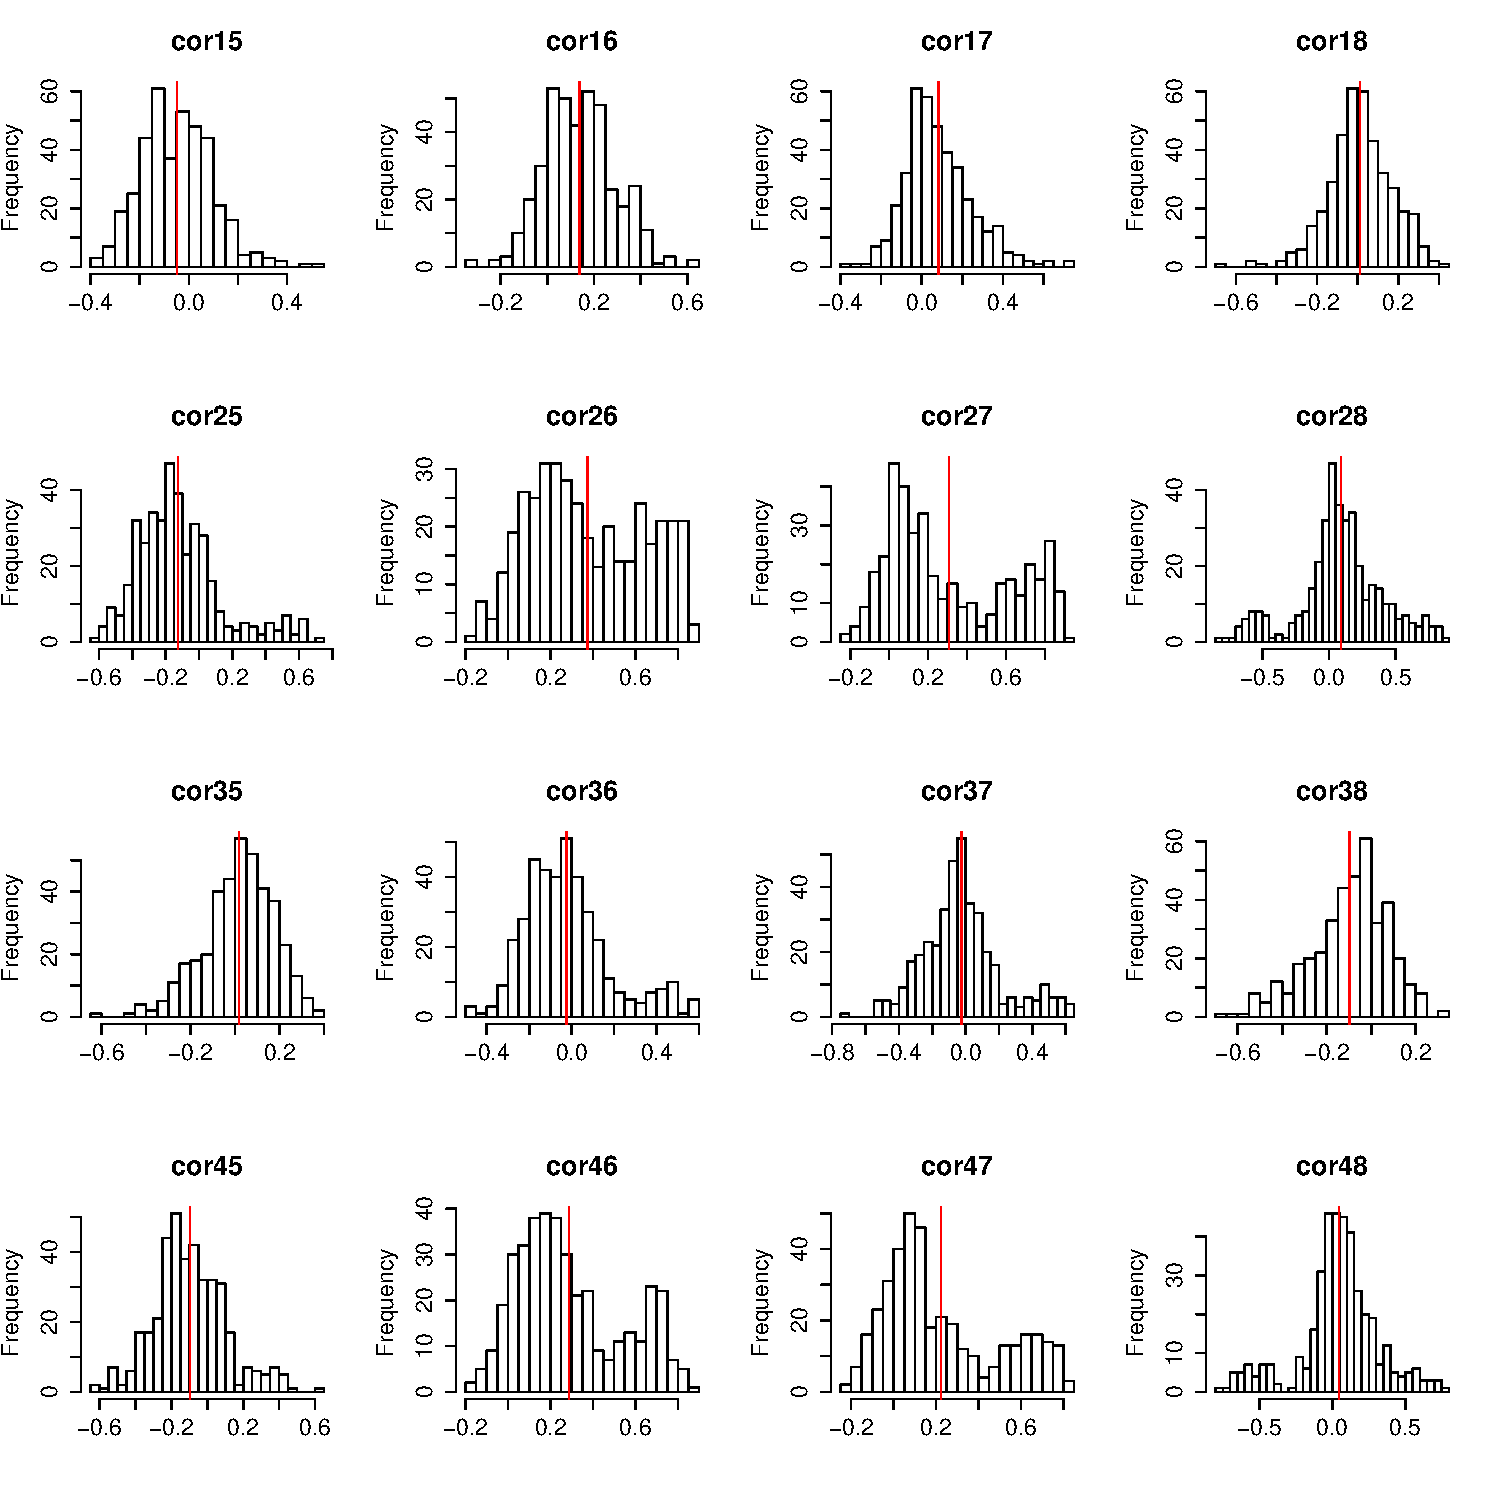
\includegraphics[width=0.35\textwidth]{Figures/PartII/Modeling/CorrelatedData/hist_crossCorMat_breaks30}
%\caption{}
}
\subfloat[]{%[t]{0.23\linewidth}
\vspace{-6.5cm}
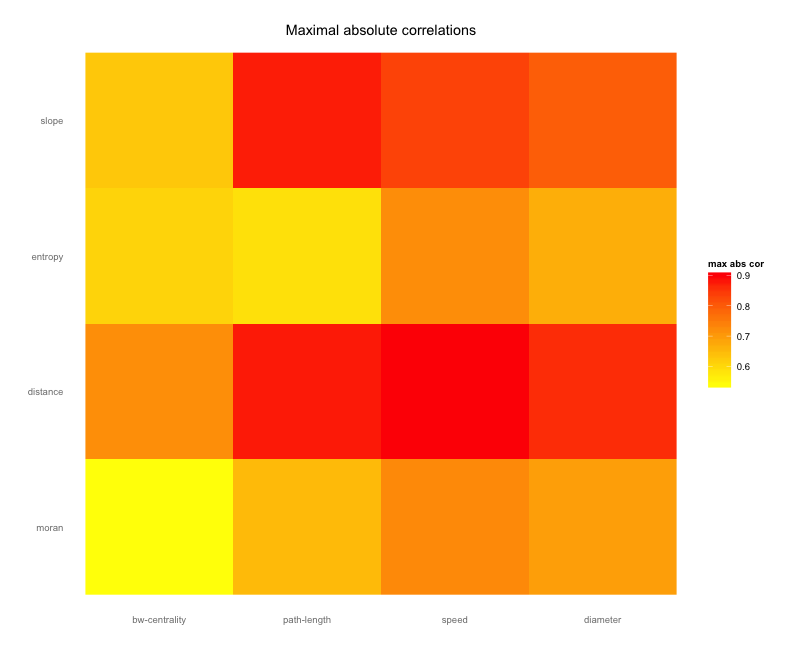
\includegraphics[width=0.23\textwidth]{Figures/PartII/Modeling/CorrelatedData/heatmap_maxAbsCor}\\
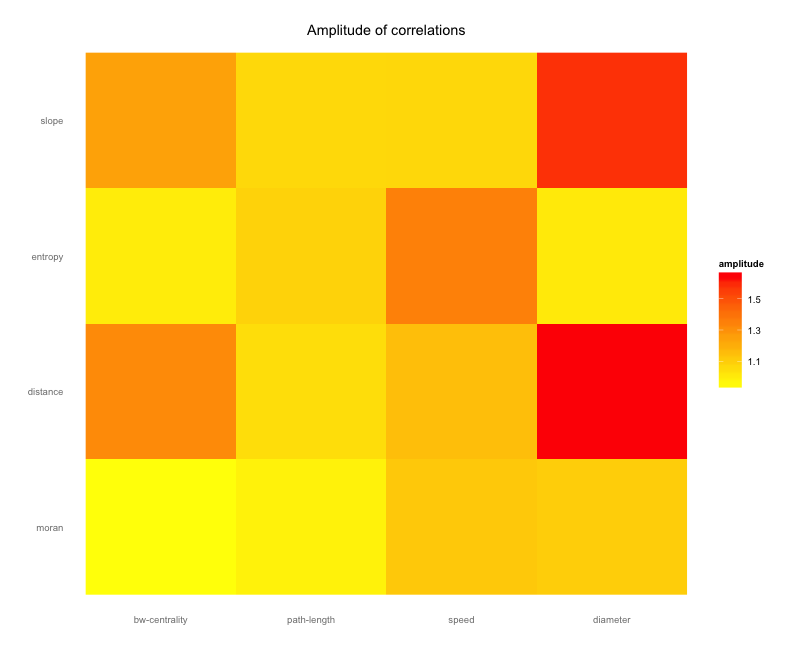
\includegraphics[width=0.23\textwidth]{Figures/PartII/Modeling/CorrelatedData/heatmap_amplCor}
}
\subfloat[]{%[t]{0.4\linewidth}
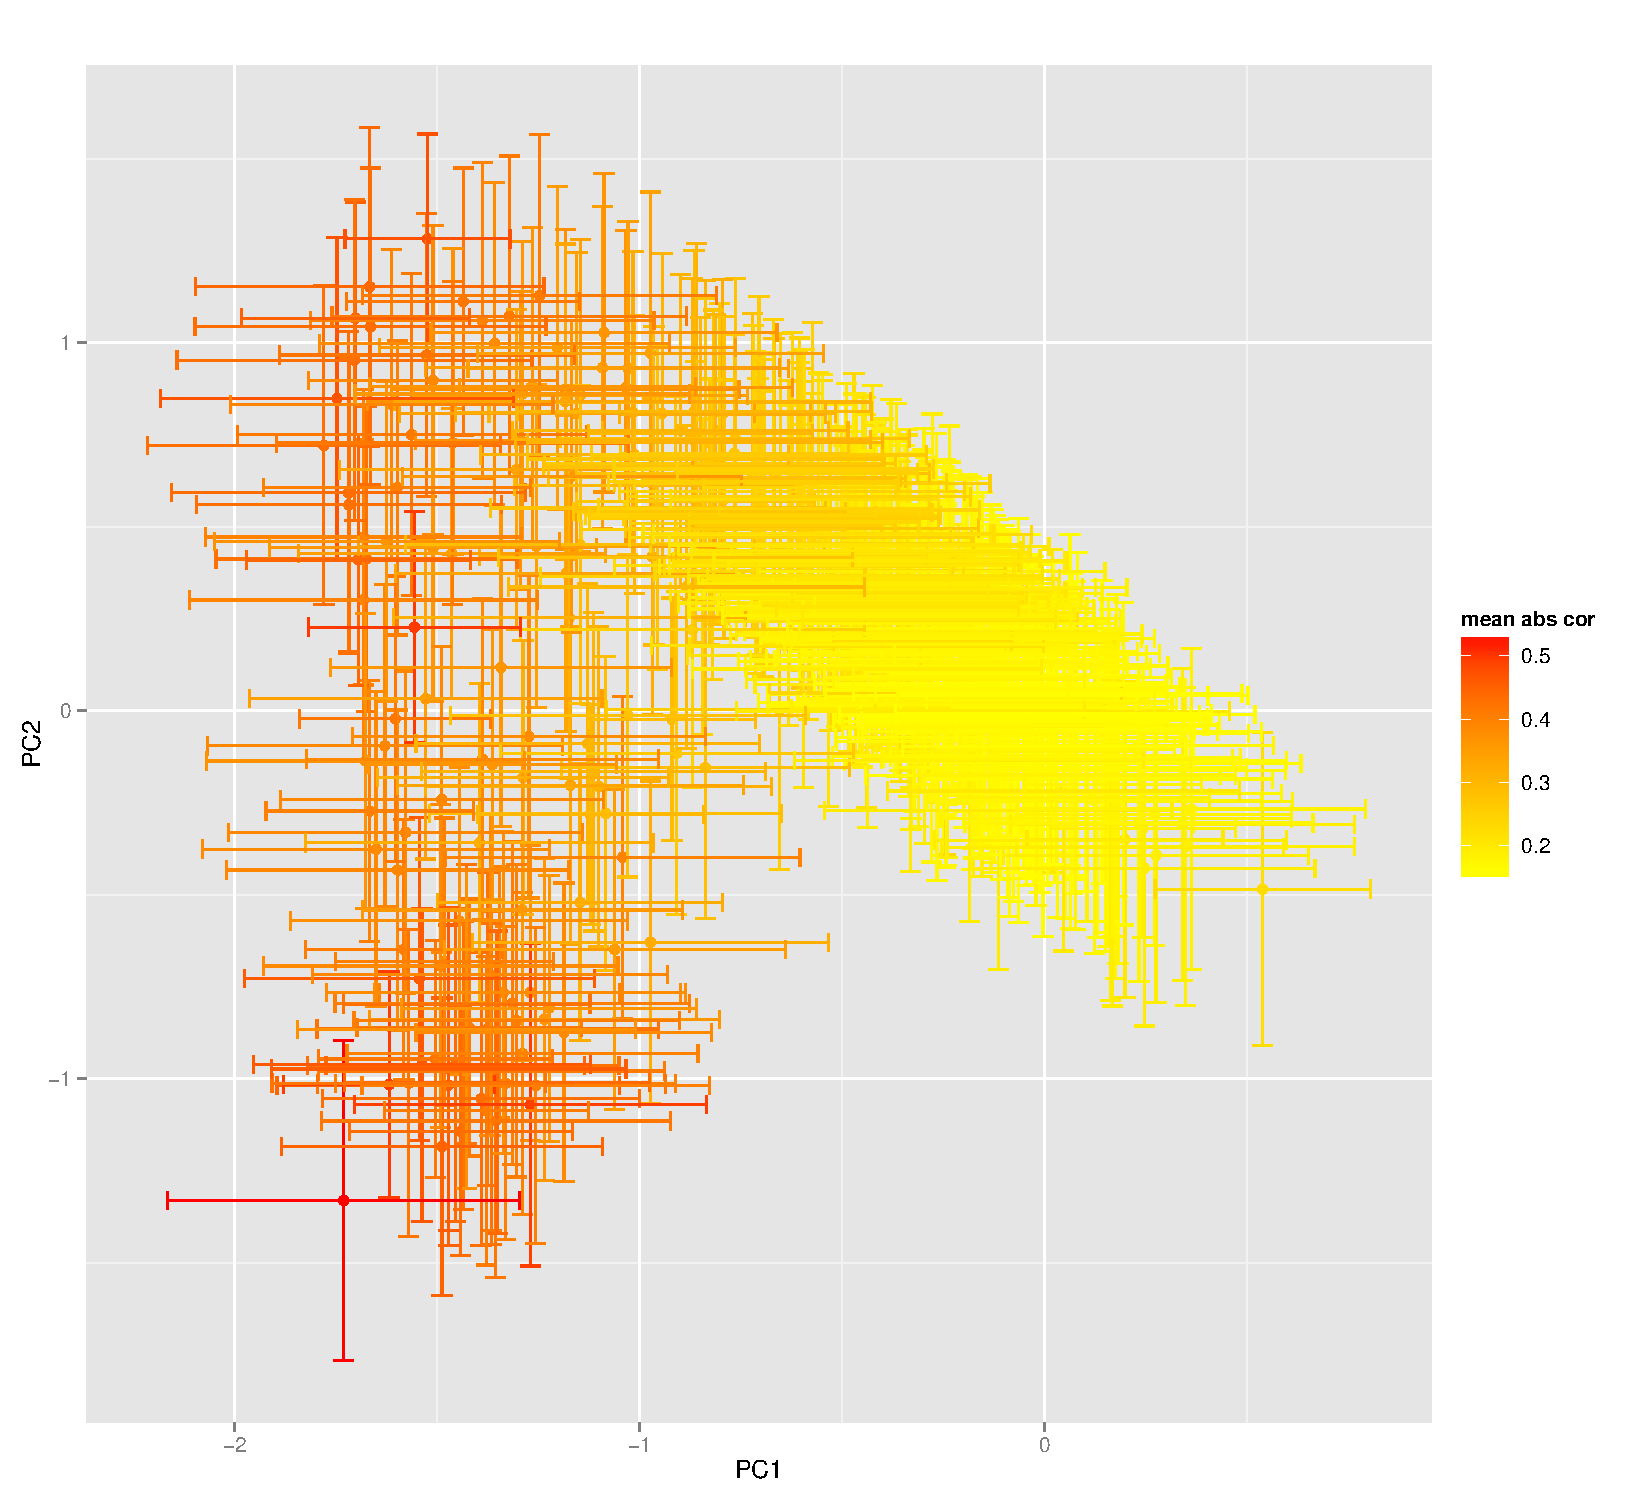
\includegraphics[width=0.4\textwidth]{Figures/PartII/Modeling/CorrelatedData/pca_meanAbsCor_errorBars}
}\\
\subfloat[]{%[t]{0.54\linewidth}
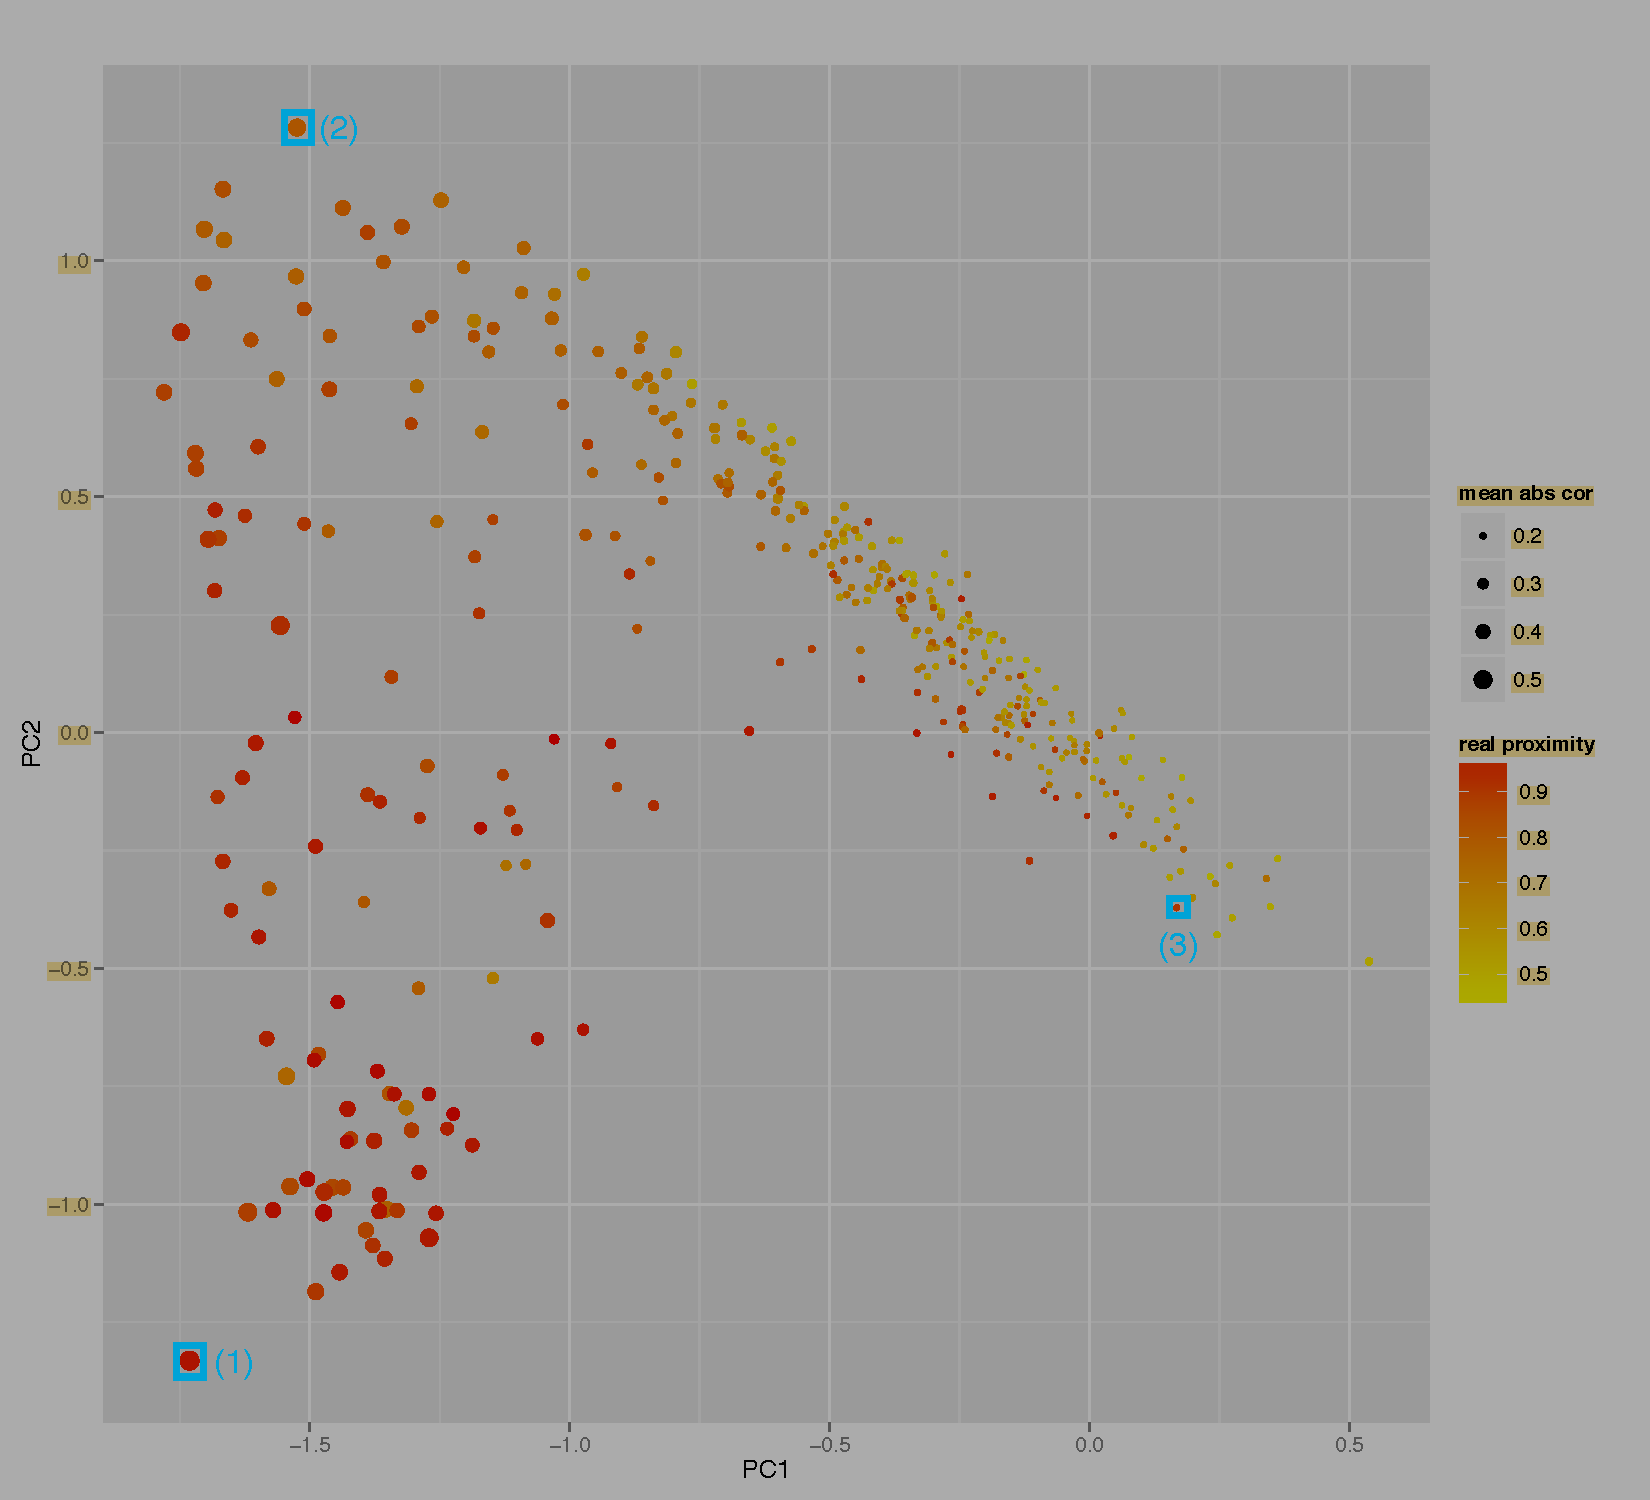
\includegraphics[width=\textwidth]{Figures/PartII/Modeling/CorrelatedData/pca_realDistCol_meanAbsCorSize_withSpecificPoints}
}
\subfloat[]{%[t]{0.45\linewidth}
\vspace{-8.3cm}
}

\caption[Exploration of feasible space for correlations between urban morphology and network structure]{\footnotesize\textbf{Exploration of feasible space for correlations between urban morphology and network structure | } \textbf{(a)} Distribution of crossed-correlations between vectors $\vec{M}$ of morphological indicators (in numbering order Moran index, mean distance, entropy, hierarchy) and $\vec{N}$ of network measures (centrality, mean path length, speed, diameter). \textbf{(b)} Heatmaps for amplitude of correlations, defined as $a_{ij}=\max_k{\rho_{ij}^{(k)}}-\min_k{\rho_{ij}^{(k)}}$ and maximal absolute correlation, defined as $c_{ij}=\max_k\left| \rho_{ij}^{k} \right|$. \textbf{(c)} Projection of correlation matrices in a principal plan obtained by Principal Component Analysis on matrix population (cumulated variances: PC1=38\%, PC2=68\%). Error bars are initially computed as 95\% confidence intervals on each matrix element (by standard Fisher asymptotic method), and upper bounds after transformation are taken in principal plan. Scale color gives mean absolute correlation on full matrices. \textbf{(d)} Representation in the principal plan, scale color giving proximity to real data defined as $1 - \min_r \norm{\vec{M}-\vec{M}_r}$ where $\vec{M}_r$ is the set of real morphological measures, point size giving mean absolute correlation.}
\label{fig:densnwcor}
\end{figure}
%%%%%%%%%%%%%%


%%%%%%%%%%%%%%
\begin{figure}
\centering

   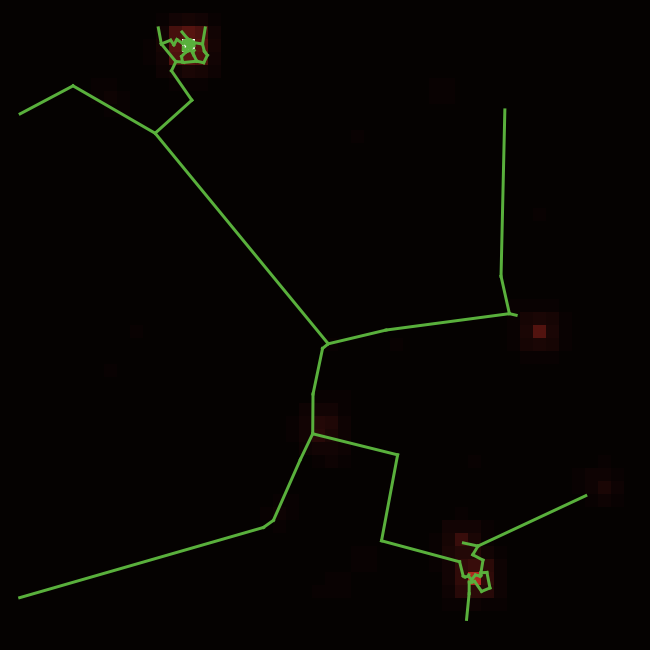
\includegraphics[width=0.5\textwidth]{Figures/PartII/Modeling/CorrelatedData/configs/1_param71861_seed0}
   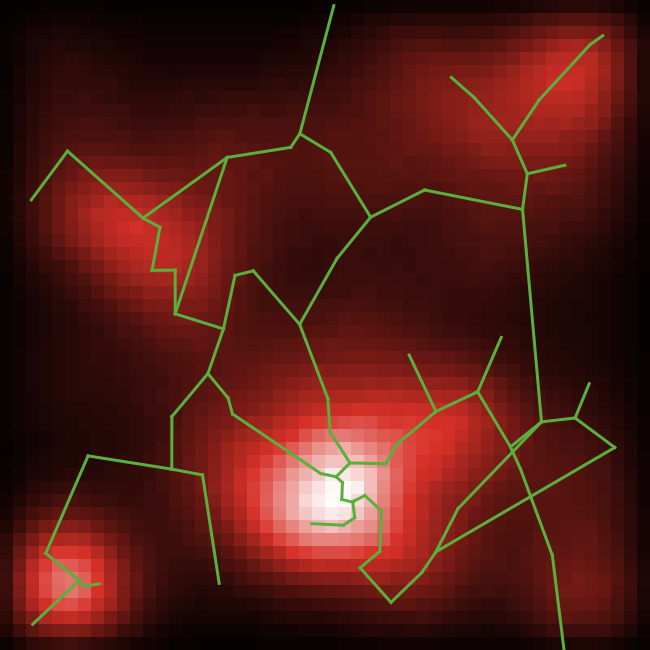
\includegraphics[width=0.5\textwidth]{Figures/PartII/Modeling/CorrelatedData/configs/2_param71913_seed10}\\
   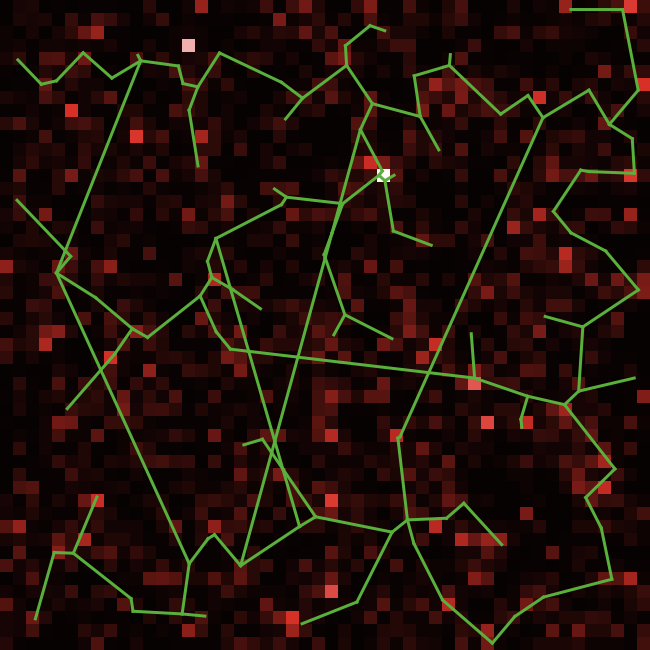
\includegraphics[width=0.5\textwidth]{Figures/PartII/Modeling/CorrelatedData/configs/3_param71918_seed0}
   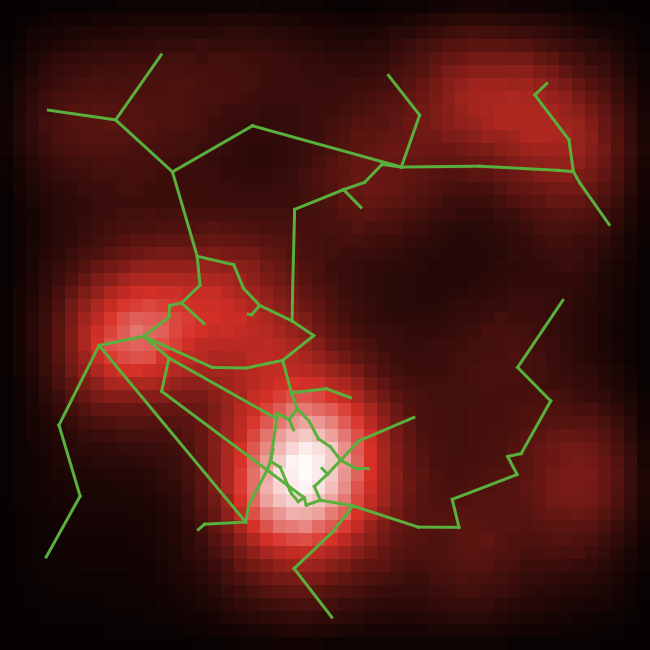
\includegraphics[width=0.5\textwidth]{Figures/PartII/Modeling/CorrelatedData/configs/4_param71945_seed0}
\caption[Examples of generated coupled configurations]{Configurations obtained for parameters giving the four emphasized points in (d), in order from left to right and top to bottom. We recognize polycentric city configurations (2 and 4), diffuse rural settlements (3) and aggregated weak density area (1). See appendice for exhaustive parameter values, indicators and corresponding correlations. For example $\bar{d}$ is highly correlated with $\bar{l},\bar{s}$ ($\simeq$0.8) in (1) but not for (3) although both correspond to rural environments ; in the urban case we observe also a broad variability : $\rho[\bar{d},\bar{c}]\simeq 0.34$ for (4) but $\simeq-0.41$ for (2), what is explained by a stronger role of gravitation hierarchy in (2) $\gamma=3.9,k_h=0.7$ (for (4), $\gamma=1.07,k_h=0.25$), whereas density parameters are similar.}
\end{figure}
%%%%%%%%%%%%%%





%%%%%%%%%%%%%%%%%%%%%%
\subsubsection{Results}

The study of density model alone is developed in~\cite{raimbault2016calibration}. It is in particular calibrated on European density grid data, on 50km width square areas with 500m resolution for which real indicator values have been computed on whole Europe. Furthermore, a grid exploration of model behavior yields feasible output space in reasonable parameters bounds (roughly $\alpha \in [0.5,2],N_G\in [500,3000], P_m \in [10^4,10^5],\beta\in [0,0.2], n_d \in \{ 1, \ldots , 4\}$). The reduction of indicators space to a two dimensional plan through a Principal Component Analysis (variance explained with two components $\simeq 80\%$) allows to isolate a set of output points that covers reasonably precisely real point cloud. It confirms the ability of the model to reproduce morphologically the set of real configurations.



% NOT NEEDED - TOO MUCH INFORMATION - ?
%%%%%%%%%%%%%%%%
%\begin{figure}
% figure : density example, exploration and calibration ?
%\end{figure}
%%%%%%%%%%%%%%%%

At given density, the conditional exploration of network generation model parameter space suggest a good flexibility on global indicators $\vec{G}$, together with good convergence properties. For a precise study of model behavior, see appendice giving regressions analysis capturing the behavior of coupled model. In order to illustrate synthetic data generation method, the exploration has been oriented towards the study of cross-correlations.


%A densité donnée, l'exploration de l'espace des paramètres du modèle de réseau suggèrent une assez bonne flexibilité sur des indicateurs globaux $\vec{G}$, ainsi que de bonnes propriétés de convergence. Pour une étude du comportement précis, voir l'appendice donnant les regressions traduisant le comportement du modèle couplé. Dans le but d'illustrer la méthode de génération de données synthétiques, l'exploration a été orientée vers l'étude des correlations.


Given the large relative dimension of parameter space, an exhaustive grid exploration is not possible. We use a Latin Hypercube sampling procedure with bounds given above for $\vec{\alpha}_D$ and for $\vec{\alpha}_N$, we take $N_C \in [50,120], r_g \in [1,100] , d_0 \in [0.1,10] , k_h \in [0,1] , \gamma \in [0.1,4],N_L\in [4,20]$. For number of model replications for each parameter point, less than 50 are enough to obtain confidence intervals at 95\% on indicators of width less than standard deviations. For correlations a hundred give confidence intervals (obtained with Fisher method) of size around 0.4, we take thus $n=80$ for experiments. Figure~\ref{fig:densnwcor} gives details of experiment results. Regarding the subject of correlated synthetic data generation, we can sum up the main lines as following :
\begin{itemize}
\item Empirical distributions of correlation coefficients between morphology and network indicators are not simple and some are bimodal (for example $\rho_{46}=\rho[r,\bar{l}]$  between Moran index and mean path length).
\item it is possible to modulate up to a relatively high level of correlation for all indicators, maximal absolute correlation varying between 0.6 and 0.9. Amplitude of correlations varies between 0.9 and 1.6, allowing a broad spectrum of values. Point cloud in principal plan has a large extent but is not uniform : it is not possible to modulate at will any coefficient as they stay themselves correlated because of underlying generation processes. A more refined study at higher orders (correlation of correlations) would be necessary to precisely understand degrees of freedom in correlation generation.
\item Most correlated points are also the closest to real data, what confirms the intuition and stylized fact of a strong interdependence in reality.
\item Concrete examples taken on particular points in the principal plan show that similar density profiles can yield very different correlation profiles.
\end{itemize}




%%%%%%%%%%%%%%
%\begin{table}
%regression analysis of param influence on correlations
%  -> Appendice.
%\end{table}
%%%%%%%%%%%%%%




\subsubsection{Possible developments}


This case study could be refined by extending correlation control method. A precise knowledge of $N$ behavior (statistical distributions on an exhaustive grid of parameter space) conditional to $D$ would allow to determine $N^{<-1>} | D$ and have more latitude in correlation generation. We could also apply specific exploration algorithms to reach exceptional configurations realizing an expected correlation level, or at least to obtain a better knowledge of the feasible space of correlations~\cite{10.1371/journal.pone.0138212}.




%%%%%%%%%%%%%%%%%%%%%%
\subsection{Discussion}
%%%%%%%%%%%%%%%%%%%%%%



%%%%%%%%%%%%%%%%%%%%%%
\subsection*{Scientific positioning}

% données hybrides au centre de la démarche d'exploration de modèle, analyse de sensitivité etc.

Our overall approach enters a particular epistemological frame. On the one hand the multidisciplinary aspect, and on the other hand the importance of empirical component through computational exploration methods, make this approach typical of Complex Systems science, as it is recalled by the roadmap for Complex Systems having a similar structure~\cite{2009arXiv0907.2221B}. It combines transversal research questions (horizontal integration of disciplines) with the development of heterogeneous multi-scalar approaches which encounter similar issues as the one we proposed to tackle (vertically integrated disciplines). The combination of empirical knowledge obtained from data mining, with knowledge obtained by modeling and simulation is generally central to the conception and exploration of multi-scalar heterogeneous models. Results presented here is an illustration of such an hybrid paradigm.




%%%%%%%%%%%%%%%%%%%%%%
\subsection*{Direct applications}


Starting from the second example which was limited to data generation, we propose examples of direct applications that should give an overview of the range of possibilities.

%En partant du deuxième exemple, qui s'est arrêté à la génération des données synthétiques, on peut proposer des pistes d'application directe qui donneront un aperçu de l'éventail des possibilités.

\begin{itemize}
\item Calibration of network generation component at given density, on real data for transportation network (typically road network given the shape of generated networks ; it should be straightforward to use OpenStreetMap open data\footnote{\texttt{https://www.openstreetmap.org}} that have a reasonable quality for Europe, at least for France~\cite{girres2010quality}, with however adjustments on generation procedure in order to avoid edge effects due its restrictive frame, for example by generating on an extended surface to keep only a central area on which calibration would be done) should theoretically allow to unveil parameter sets reproducing accurately existing configurations both for urban morphology and network shape. It could be then possible to derive a ``theoretical correlation'' for these, as an empirical correlation is according to some theories of urban systems not computable as a unique realization of stochastic processes is observed. Because of non-ergodicity of urban systems~\cite{pumain2012urban}, there are strong chances that involved processes are different across different geographical areas (or from an other point of view that they are in an other state of meta-parameters, i.e. in an other regime) and that their interpretation as different realizations of the same stochastic process makes no sense, the impossibility of covariation estimation following. By attributing a synthetic dataset similar to a given real configuration, we would be able to compute a sort of \emph{intrinsic correlation} proper to this configuration. As territorial configurations emerge from spatio-temporal interdependences between components of territorial systems, this intrinsic correlation emerges the same way, and its knowledge gives information on these interdependences and thus on relations between territories and networks.
\item As already mentioned, most of models of simulation need an initial state generated artificially as soon as model parametrization is not done completely on real data. An advanced model sensitivity analysis implies a control on parameters for synthetic dataset generation, seen as model meta-parameters~\cite{cottineau2015revisiting}. In the case of a statistical analysis of model outputs it provides a way to operate a second order statistical control.
\item We studied in the first example stochastic processes in the sense of random time-series, whereas time did not have a role in the second case. We can suggest a strong coupling between the two model components (or the construction of an integrated model) and to observe indicators and correlations at different time steps during the generation. In a dynamical spatial models we have because of feedbacks necessarily propagation effects and therefore the existence of lagged interdependences in space and time~\cite{pigozzi1980interurban}. It would drive our field of study towards a better understanding of dynamical correlations.
\end{itemize}




%%%%%%%%%%%%%%%%%%%%%%
\subsection*{Generalization}

We were limited to the control of first and second moments of generated data, but we could imagine a theoretical generalization allowing the control of moments at any order. However, as shown by the geographical example, the difficulty of generation in a concrete complex case questions the possibility of higher orders control when keeping a consistent structure model and a reasonable number of parameters. The study of non-linear dependence structures as proposed in~\cite{chicheportiche2013nested} is in an other perspective an interesting possible development.



%%%%%%%%%%%%%%%%%%%%%%
%\subsection*{Autres domaines potentiels d'application}
% ideas of other fields where the generation can happen.
% -> not necessary, suggested in intro ?



%%%%%%%%%%%%%%%%%%%%%%
\subsection{Conclusion}
%%%%%%%%%%%%%%%%%%%%%%


We proposed an abstract method to generate synthetic datasets in which correlation structure is controlled. Its rapid implementation in two very different fields shows its flexibility and the broad range of possible applications. More generally, it is crucial to favorise such practices of systematic validation of computational models by statistical analysis, in particular for agent-based models for which the question of validation stays an open issue.







%--------------------------------------

% Section : benchmarking of network growth models

\newpage

\section[Network Growth Models]{Network Growth Models : Explicative power for various approaches}

Considering Network Growth in itself, many heuristics are available to generate a network under some constraints. As already developed, 

















% Lutecia : particular case including specific thematic developments





% Chapter 

\chapter{Towards more Complex Models} % Chapter title

\label{ch:complexmodels} % For referencing the chapter elsewhere, use \autoref{ch:name} 


%----------------------------------------------------------------------------------------

This single section chapter is differentiated from the previous one as it makes a step further towards more complex models. A toy-model introducing governance processes is described. Such exploration logically enters our theoretical framework to try to validate or invalidate the network necessity assumption : if non-linear necessary processes are highlighted and validated against stylized facts, it argues towards the validation of this assumption. 

Other targeted projects such as the exploration of an hybrid macro-economic/accessibility-based model to explore transportation companies line implementation strategies are still at the state of ideas and are not described here.



%----------------------------------------------------------------------------------------


\section[The Lutecia Model]{Taking Governance into account in Network Production Processes : The Lutecia Model}


%%%%%%%%%%%%%%%%%%
\subsection{Thematic Context}


We briefly describe a simple game-theory based framework, conjointly done with \noun{Le Nechet} which aims to be integrated as behavioral rules for governing agents in a hybrid model introduced in~\cite{le2010approche} and formalized then explored in~\cite{lenechet2012}. This model couples land-use dynamics with transportation infrastructure evolution and aims to endogeneize transportation infrastructure development at different levels. The framework proposed extends it by allowing cooperation and fusion between governing entities.



As detailed in~\cite{lenechet2012}, a conceptual city system with local administrative boundaries and corresponding governing agents (mayors), and a global governor (state) is the foundation of the model. A land-use evolution (residences and employments localisations) and transportation (gravity flows) are the first step of an iteration. The transportation infrastructure (road network) is then evolved by constructing a new road. First level of decision (global or local) is chosen randomly according to a fixed probability, and in the case of a local decision, the richest mayor will build the new road. The road is then build optimizing the marginal accessibility for the area corresponding to the builder in charge (all world if global, commun if local).

One thematic aspect lacking in the model and that would be interesting to study is the emergence of larger administrative zones, i.e. the emergence of new levels of governance in polycentric metropolitan areas. The reality is of course not as simple, as bottom-up initiatives such as collaboration between neighbor cities are interlaced with top-down decisions such as e.g. the ``M{\'e}tropole du Grand Paris'' which is a new administrative structure for Paris Area decided at the state level~\cite{gilli2009paris}. It would be however interesting to test conditions for emergence of governance patterns from the bottom-up in a conceptual way by extending the model and adding interactions and fusion between administrative entities.

The extension shall consist in relaxing the assumption of a single road segment built at each time step and attribute one segment to the $N$ richest mayors. That leads to situation where neighbor towns may want to construct both a new road. As they are likely to communicate with each other, we assume that negotiations take place and that they consider eventually to build in common, in which case they merge after (rough simplifying but stylized assumption). Such negotiations may be interpreted as a game in the sense of Game Theory, which as already been widely applied for modeling in social and political sciences for questions dealing with cognitive interacting agents with individual interests~\cite{ordeshook1986game}. Such a framework as already been used in transportation investment studies, as e.g. in~\cite{Roumboutsos2008209} where choices of operators (public and privates) to integrate their system in a global consistent commuter system is explored through the notion of Nash equilibrium.

% \cite{2016arXiv161208111S} : rationale for staying at two players : games with many become chaotic




\subsection{Formalization}


The model architecture couples in a complex way a module for land-use evolution with a module for transportation network growth. Submodules, detailed in the following, include in particular a governance module that rules processes of network evolution.


\subsubsection{Land-use evolution}

The following steps are detailed in~\cite{lenechet2012} but we recall the big picture :

\begin{itemize}
\item Initial distribution of Actives and Employments is done around governance centers at positions $\vec{x}_i$ by
\[
A(\vec{x}) = A_{max} \cdot \exp{\left(\frac{\norm{\vec{x}-\vec{x}_i}}{r_A}\right)} ; 
E(\vec{x}) = E_{max} \cdot \exp{\left(\frac{\norm{\vec{x}-\vec{x}_i}}{r_E}\right)}
\]

\item For facility patches, employments are added by $E(\vec{x}) = E(\vec{x})+\frac{k_{ext}\cdot E_{max}}{n_{ext}}$.

\item Transportation module : computation of flows $\phi_{ij}$ are done by solving on $p_i,q_j$ by a fixed point method (Furness algorithm), the system of gravity flows
\[
\begin{cases}
\phi_{ij} = p_i q_j A_i E_j \exp{\left(-\lambda_{tr} d_{ij}\right)}\\
\sum_k \phi_{kj} = E_j ; \sum_k \phi_{ik} = A_i\\
p_i = \frac{1}{\sum_k{q_k E_k \exp{(-\lambda_{tr}d_{ik})}}} ; q_j = \frac{1}{\sum_k{p_k A_k \exp{(-\lambda_{tr}d_{kj})}}} 
\end{cases}
\]

\item Trajectories then attributed by effective shortest path, and corresponding congestion $c$ obtained (no Wardrop equilibrium). 

\item Speed of network is given by a BPR function $v(c) = v_0 \left(1 - \frac{c}{\kappa}\right)^{\gamma_c}$. Congestion is not used in current studies (infinite capacity $\kappa$).

\item Land-Use module : we assume that residential/employments relocations are at equilibrium at the time scale of a tick, that corresponds to transportation infrastructure evolution time scale which is much larger~\cite{bretagnolle:tel-00459720}.

\item We take a Cobb-douglas function for utilities of actives/employments at a given cell
\[
U_i (A) = X_i(A)^{\gamma_A}\cdot {F_i(A)}^{1-\gamma_A} ; F_i(A) = \frac{1}{A_i E_i}
\]
\[
U_j (E) = X_j(E)^{\gamma_E}\cdot {F_j(E)}^{1-\gamma_E} ; F_j(E) = 1
\]

where $X_i(A) = A_i\cdot \sum_j{E_j \exp{\left(-\lambda\cdot d_{ij}\right)}}$ and $X_j(E) = E_j\cdot \sum_i{A_i \exp{\left(-\lambda\cdot d_{ij}\right)}}$.

\item Relocations are then done deterministically following a discrete choice model :
\[
A_i(t+1) = \sum_i{A_i(t)}\cdot\frac{\exp{(\beta U_i(A))}}{\sum_i{\exp{(\beta U_i(A))}}}
\]
\[
E_j(t+1) = \sum_j{E_j(t)}\cdot\frac{\exp{(\beta U_j(E))}}{\sum_j{\exp{(\beta U_j(E))}}}
\]

\end{itemize}


The default parameter values are taken as follows : $A_{max} = E_{max} = 500 ; r_A = 1 ; r_E = 0.8 ; \gamma_E = 0.9 ; \gamma_A = 0.65 ; \beta_{l} = 1.8 ; \lambda = 0.005 ; r_0 = 2$

and 
 
$N_{expl} = 25 ; I = 0.001 ; J = 0.0001 ; \nu = 5 ; E_{ext}(t_0) = 3E_{max} ; t_f = 4$


%%%%%%%%%%%%%%%%%%%%%
%% Dynamic programming
%%%%%%%%%%%%%%%%%%%%%

\subsubsection{Effective distances computation}

Distance via network are updated in a dynamical programming fashion for efficiency purposes (because of the numerous network updates), the following way :

\begin{itemize}
\item Euclidian distance matrix $d(i,j)$ computed analytically
\item Network shortest paths between network intersections (rasterized network) updated in a dynamic way (addition of new paths and update/change of old paths if needed when a link is added), correspondance between network patches and closest intersection also updated dynamically ; $O(N_{inters}^3)$
\item Weak component clusters and distance between clusters updated ; $O(N_{nw}^2)$
\item Network distances between network patches updated, through the heuristic of only minimal connexions between clusters ; $O(N_{nw}^2)$
\item Effective distances (taking paces/congestion into account) updated as minimum between euclidian time and \[\min_{C,C'}{d(i,C)+d_{nw}(p_C(i),p_C'(j))+d(C',j)}\], complexity in $O(N_{clusters}^2\cdot N^2)$ (Approximated with $\min_C$ only in the implementation, consistent within the interaction ranges $\sim$ 5 patches taken in the model). 
\end{itemize}



\subsubsection{Externality}

The model allows also to simulate the competition of territory for an external ressource (an airport for example). We implement therefore the option of adding in initial state an area with initial $A_{max}$ employments and that follows an intrinsic growth rule as a geometric law. 



\subsubsection{Transportation Network growth}


The workflow for transportation network development is the following :

\begin{itemize}

\item At each time step, $N$ new road segments are built. Choice between local and global is still done through uniform drawing with probability $\xi$. In the case of local building, roads are attributed successively to mayors with probabilities $\xi_i$, what means that richer areas may get many roads. It stays consistent with the thematic assumption than each road correspond to the allocation of one public market which are done independently (with $N$ becoming greater, this assumption should be relaxed as attribution of subventions to local areas is of course not proportional to wealth, but we assume that it stays true with small $N$ values). 

\item Areas building a road without neighbors doing it follow the standard procedure to develop the road network.

\item Neighbor areas building a road will enter negotiations. We assume in this first simple version of the model that only bilateral negotiations may occur. Therefore, in the case of clusters with more than two areas, pairing is done at random (uniform drawing) between neighbors until all areas are paired.

\item Possible strategies for players (negotiating areas, $i=1,2$) are : staying alone ($A$) and collaborating ($C$). Strategies are chosen simultaneously (non-cooperative game) as detailed after. For $(C,A)$ and $(A,C)$ couples, the collaborating agent loose its investment and cannot build a road whereas the other continues his business alone. For $(A,A)$ both act as alone, and for $(C,C)$ a common development is done. We denote $Z^{\ast}_i(S_1,S_2)$ the optimal infrastructure for area $i$ with $(S_1,S_2)\in \{(A,C),(C,A),(A,A)\}$ which are determined the standard way in each zone separately, and $Z^{\ast}_C$ the optimal common infrastructure computed with a 2 segments infrastructure on the union of both areas, which corresponds to the case where both strategies are $C$. Marginal accessibilities for area $i$ and infrastructure $Z$ is defined as $\Delta X_i(Z)=X^Z_i - X_i$. We introduce the costs of construction which are necessary to build the payoff matrix. They are assumed spatially uniform and noted $I$ for a road segment, whereas a 2 road segment will cost $2\cdot I - \delta I$ ($\delta I > 0$ cost gain of common technical means, assumed to be equally shared). An interesting generalization would be to divise costs proportional to wealth in the case of a collaboration. The payoff matrix of the game is the following, with $\kappa$ a normalization constant (``price of accessibility'') :

\medskip
\hfill
\begin{tabular}{ |c|c|c| } 

 \hline
 1 $|$ 2  & C & A \\ \hline
 C & $U_i = \kappa \cdot \Delta X_i(Z^{\ast}_C) - I - \frac{\delta I}{2}$
   & $\begin{cases}U_1 = \kappa \cdot \Delta X_1(Z^{\ast}_1)-I \\U_2 = \kappa \cdot \Delta X_2(Z^{\ast}_2)-I - \frac{\delta I}{2}\end{cases}$ \\ \hline
 A & $\begin{cases}U_1 = \kappa \cdot \Delta X_1(Z^{\ast}_1)-I - \frac{\delta I}{2}\\U_2 = \kappa \cdot \Delta X_2(Z^{\ast}_2)-I\end{cases}$
   & $U_i = \kappa \cdot \Delta X_i(Z^{\ast}_i) - I$ \\
 \hline
\end{tabular}
\hfill\hfill
\medskip

We have a typical coordination game for which it is clear that no strategy is dominant for any player. In a probabilistic mixed-strategy case, there always exists a Nash equilibrium that we can easily determine in our case. It is reasonable to make such an assumption since negotiations take generally some time during which agents are able to find the way to optimize rationally their expected utility. If $\Pb{S_1=C} = p_1$ and $\Pb{S_2=C} = p_2$, we have

\[
\begin{split}
\Eb{U_1} & =p_1 p_2 U_1(C,C) + p_1\cdot (1-p_2) U_1(C,A) + p_2 \cdot (1-p_1) U_1(A,C) + (1-p_1)(1-p_2) U_1(A,A)\\
& = p_1 \cdot \left[ p_2 \cdot \left(\kappa \cdot \Delta X_1(Z^{\ast}_C) - \frac{\delta I}{2} \right) - \kappa \cdot \Delta X_1(Z^{\ast}_1) + I\right] + p_2\cdot\frac{\delta I}{2} + \kappa\cdot\Delta X_1(Z^{\ast}_1)-I
\end{split}
\]

Optimizing the expected utility along $p_1$ (the variable on which agent 1 has control) imposes the condition on $p_2$

\[
\frac{\partial \Eb{U_1}}{\partial p_1} = 0 \iff p_2 = \frac{\delta I / 2}{\Delta X_{\bar{2}}{Z^{\star}_{C}} - \Delta X_{\bar{2}}{Z^{\star}_{\bar{2}}}}
\]

We obtain generally

\[
p_i = \frac{J}{\Delta X_{\bar{i}}{Z^{\star}_{C}} - \Delta X_{\bar{i}}{Z^{\star}_{\bar{i}}}}
\]

Note that we can directly interpret these expressions, as a player chances to cooperate will decrease with the potential gain of the other player, what is intuitive for a competitive game. It also forces feasibility conditions on $I$ and $\delta I$ to keep a probability, that are $I \leq \kappa\cdot \min(\Delta X_1(Z^{\ast}_1),\Delta X_2(Z^{\ast}_2))$ (binary positive cost-benefit conditions) and $I-\delta I > \kappa \cdot \max_i (\Delta X_i(Z^{\ast}_i)-\Delta X_i(Z^{\ast}_C))$. As soon as accessibility difference stay relatively small, both shall be compatible when $\delta I \ll I$, giving corresponding boundaries for $I$.

\item Agents make choice of strategy following uniform drawings with probability computed above. Corresponding infrastructures are built, and in the case of choices $(C,C)$, towns merge in a single one with new corresponding variables (employment, actives, etc. ).


\end{itemize}



\paragraph{Remark for the implementation}

To adapt an existing implementation, one just has to add the negotiation stage if conditions are met, using probabilities given above. The accessibility-dimensioned parameters $\alpha = \frac{I}{\kappa}$ and $\delta \alpha = \frac{\delta I}{\kappa}$ should be more simple to deal with.



% TODO : insert a mechanisms with NO DC framework as reference/benchmark/null model ?

\paragraph{An alternative discrete choice ``game''}

Using the same payoff matrix with a random utility model allows to obtain also values for probabilities. We have

\[
U_i(C) - U_i(NC) = p_{\bar{i}} \left( \Delta X_{i}{Z^{\star}_{C}} - \Delta X_{i}{Z^{\star}_{i}}\right) - J
\]

and therefore $p_i$ verifies the equation that is solved numerically

\[
p_i = \frac{1}{1 + \exp{\left(-\beta_{DC}\cdot \left(\frac{\Delta X_{i}{Z^{\star}_{C}} - \Delta X_{i}{Z^{\star}_{i}}}{1 + \exp{\left(- \beta_{DC}(p_i \cdot (\Delta X_{\bar{i}}{Z^{\star}_{C}} - \Delta X_{\bar{i}}{Z^{\star}_{\bar{i}}}) - J)\right)}} - J \right)\right)}}
\]

This module is also implemented for comparison purposes.


\subsection{Results}

% validation at different levels ; exploration etc.  - to be relaunched -

\subsubsection{Implementation}

The model was implemented in \texttt{NetLogo}~\cite{wilensky1999netlogo} because of its exploratory and interactive nature. A particular care was taken for the computation of accessibilities and shortest paths, as a dynamic reevaluation of network distance is necessary for each new potential infrastructure, what become rapidly a computational burden. We use thus a dynamical programming shortest path computation, inspired from~\cite{tretyakov2011fast}, using distance matrices updates instead of shortest paths full computation at each step. See details in architectural precisions in Appendix~\ref{app:bibliography}


%%%%%%%%%%
\begin{figure}
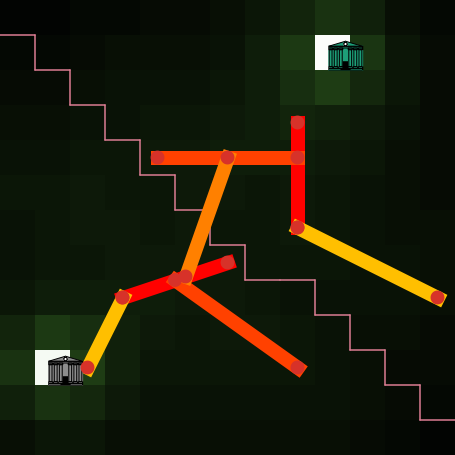
\includegraphics[width=0.5\textwidth]{Figures/PartII/Modeling/Lutecia/ex_collab_0}
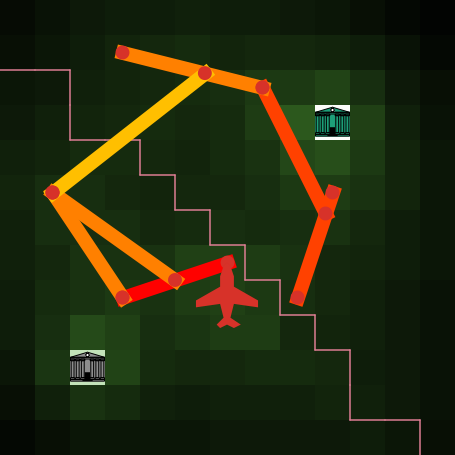
\includegraphics[width=0.5\textwidth]{Figures/PartII/Modeling/Lutecia/ex_dc_finalCollab}\\
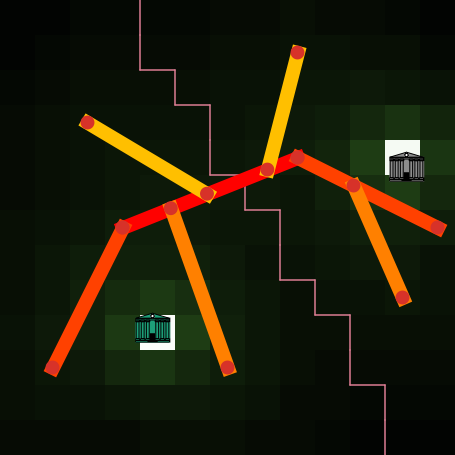
\includegraphics[width=0.5\textwidth]{Figures/PartII/Modeling/Lutecia/ex_simpleNash_0}
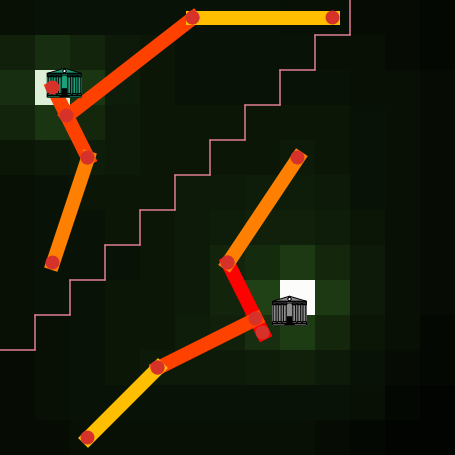
\includegraphics[width=0.5\textwidth]{Figures/PartII/Modeling/Lutecia/example_nocollab_0}
\caption[Examples of final configurations]{Examples of final configurations, with or without externality, for different values of cooperation parameters.}
\label{fig:luteciaexample}
\end{figure}
%%%%%%%%%%


%%%%%%%%%%
\begin{figure}
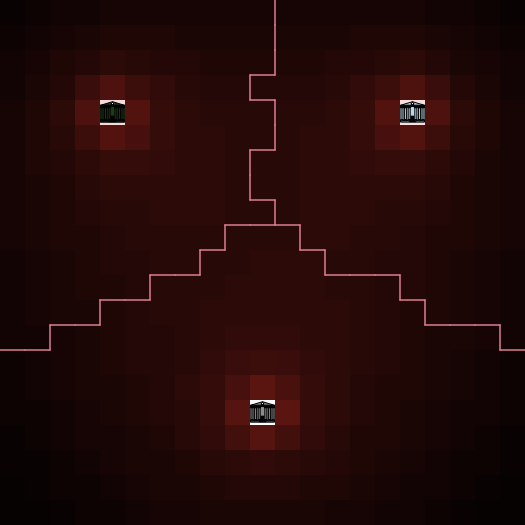
\includegraphics[width=0.5\textwidth]{Figures/PartII/Modeling/Lutecia/_MEAN_ACC}
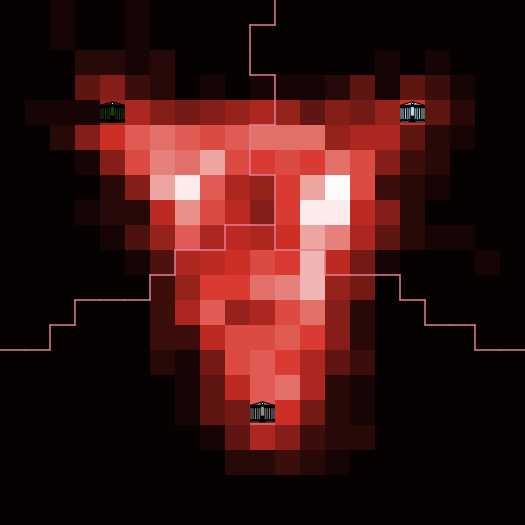
\includegraphics[width=0.5\textwidth]{Figures/PartII/Modeling/Lutecia/_NW_FREQ}
\caption[Validation of network exploration heuristic]{Validation of network exploration heuristic : mean accessibility(left) and network positions on 500 realizations on the same initial configuration. The optimal distribution of network validates network generation heuristic.}
\label{fig:luteciavalid}
\end{figure}
%%%%%%%%%%%



\subsubsection{Exploration and Validation}

We show in Fig.~\ref{fig:luteciaexample} and Fig.\ref{fig:luteciavalid} examples of obtained configurations and preliminary validation of governance and network growth heuristic. Internal validation and external validation through stylized facts, and model explorations, including statistical analysis of model behavior, are provisory for now and not presented here (see~\cite{le2015modeling} for preliminary results).


%\subsection{Perspectives}
% why is this model useful for the following













%% Chapter X

\chapter{Chapter Title} % Chapter title

\label{ch:name} % For referencing the chapter elsewhere, use \autoref{ch:name} 

%----------------------------------------------------------------------------------------

\section{Section Title}

Content

%------------------------------------------------

\subsection{Subsection Title}

Content

%------------------------------------------------

\subsection{Subsection Title}

Content

%----------------------------------------------------------------------------------------

\section{Section Title}

Content % Chapter 4 - empty template

\cleardoublepage % Empty page before the start of the next part


%------------------------------------------------

\ctparttext{} % Text on the Part 2 page describing the content in Part 2


% Part III : Towards operational models
\part{Towards operational models} % Second part of the thesis






%------------------------------------------------

\ctparttext{} % Text on the Part 2 page describing the content in Part 2


% Conclusion
\part{Conclusion} % Second part of the thesis





% 

\cleardoublepage% Bibliography

\label{app:bibliography} % Reference the bibliography elsewhere with \autoref{app:bibliography}

\manualmark % Work-around to have small caps also here in the headline
\markboth{\spacedlowsmallcaps{\bibname}}{\spacedlowsmallcaps{\bibname}} % Work-around to have small caps also
\phantomsection
\refstepcounter{dummy}

\addtocontents{toc}{\protect\vspace{\beforebibskip}} % Place the bibliography slightly below the rest of the document content in the table of contents
\addcontentsline{toc}{chapter}{\tocEntry{\bibname}}



\printbibliography % Bibliography

%----------------------------------------------------------------------------------------
%	THESIS CONTENT - APPENDICES
%----------------------------------------------------------------------------------------

\appendix

\part{Appendix} % New part of the thesis for the appendix

%% Appendix A

\chapter{Appendix Test}

%----------------------------------------------------------------------------------------

\lipsum[13-14]

%----------------------------------------------------------------------------------------

\section{Appendix Section Test}
\lipsum[15]

\graffito{More dummy text}
\lipsum[16]

%----------------------------------------------------------------------------------------

\section{Another Appendix Section Test}
\lipsum[17]

\begin{table}
\myfloatalign
\begin{tabularx}{\textwidth}{Xll} \toprule
\tableheadline{labitur bonorum pri no} & \tableheadline{que vista}
& \tableheadline{human} \\ \midrule
fastidii ea ius & germano &  demonstratea \\
suscipit instructior & titulo & personas \\
\midrule
quaestio philosophia & facto & demonstrated \\
\bottomrule
\end{tabularx}
\caption[Autem usu id]{Autem usu id.}
\label{tab:moreexample}
\end{table}

\lipsum[18]

There is also a useless Pascal listing below: \autoref{lst:useless}.

\begin{lstlisting}[float=b,language=Pascal,frame=tb,caption={A floating example (\texttt{listings} manual)},label=lst:useless]
for i:=maxint downto 0 do
begin
{ do nothing }
end;
\end{lstlisting} % Appendix A
%% Appendix X

\chapter{Appendix Title}

%----------------------------------------------------------------------------------------

% Content begins here % Appendix B - empty template

%----------------------------------------------------------------------------------------
%	POST-CONTENT THESIS PAGES
%----------------------------------------------------------------------------------------


%\cleardoublepage% Declaration

\refstepcounter{dummy}
\pdfbookmark[0]{Declaration}{declaration} % Bookmark name visible in a PDF viewer

\chapter*{Declaration} % Declaration section text

\thispagestyle{empty}

Put your declaration here.
\bigskip
 
\noindent\textit{\myLocation, \myTime}

\smallskip

\begin{flushright}
\begin{tabular}{m{5cm}}
\\ \hline
\centering\myName \\
\end{tabular}
\end{flushright}
 % Declaration

%\cleardoublepage% Colophon (a brief description of publication or production notes relevant to the edition)

\pagestyle{empty}

\hfill

\vfill

\pdfbookmark[0]{Colophon}{colophon}

\section*{Colophon}

This document was typeset using the typographical look-and-feel \texttt{classicthesis} developed by Andr\'e Miede. The style was inspired by Robert Bringhurst's seminal book on typography ``\emph{The Elements of Typographic Style}''. \texttt{classicthesis} is available for both \LaTeX\ and \mLyX: 

\begin{center}
\url{https://bitbucket.org/amiede/classicthesis/}
\end{center}

\noindent Happy users of \texttt{classicthesis} usually send a real postcard to the author, a collection of postcards received so far is featured here: 

\begin{center}
\url{http://postcards.miede.de/}
\end{center}
 
\bigskip

\noindent\finalVersionString % Colophon

%----------------------------------------------------------------------------------------

\end{document}
